\documentclass[12pt,oneside]{reedthesis}

\usepackage{graphicx,latexsym}
\usepackage{amsmath}
\usepackage{amssymb,amsthm}
\usepackage{longtable,booktabs,setspace}
\usepackage[hyphens]{url}
\usepackage{hyperref}
\hypersetup{breaklinks=true,
            bookmarks=true,
            pdfauthor={Erik Gahner Larsen and Zoltán Fazekas},
            pdftitle={Quantitative Politics with R},
            colorlinks=true,
            citecolor=blue,
            urlcolor=blue,
            linkcolor=blue,
            pdfborder={0 0 0}}
\urlstyle{same}
\usepackage{lmodern}
\usepackage{float}
\floatplacement{figure}{H}

\usepackage{rotating}

\usepackage[hmargin=3cm,vmargin=2.5cm]{geometry}
\usepackage[utf8]{inputenc}
\usepackage[T1]{fontenc}
\usepackage{multirow}
\usepackage{booktabs}
\usepackage{microtype}
\usepackage{nag}
\usepackage{cleveref}
\usepackage{float}
\usepackage{dcolumn}
\usepackage{pdflscape}
\usepackage{multirow}
\usepackage{caption}
\usepackage{footmisc}
\usepackage{pdflscape}
\usepackage{array}
\usepackage{cleveref}
\usepackage{longtable}

\renewcommand{\hyperref}[2][???]{\autoref{#1}}
\def\chapterautorefname{Chapter}
\def\sectionautorefname{Section}
\def\subsectionautorefname{Subsection}

\usepackage{caption}
\captionsetup{width=5in}

\title{\Huge{ Quantitative Politics with R } \vspace{2em}}
\author{Erik Gahner Larsen and Zoltán Fazekas}
\date{November 22, 2018}

\renewcommand{\contentsname}{Table of Contents}

\setlength{\parskip}{0pt}

% Added by CII

\providecommand{\tightlist}{%
  \setlength{\itemsep}{0pt}\setlength{\parskip}{0pt}}


% End of CII addition
%%
%% End Preamble
%%
%

\linespread{1.3}

\usepackage{amsthm}
\newtheorem{theorem}{Theorem}[section]
\newtheorem{lemma}{Lemma}[section]
\theoremstyle{definition}
\newtheorem{definition}{Definition}[section]
\newtheorem{corollary}{Corollary}[section]
\newtheorem{proposition}{Proposition}[section]
\theoremstyle{definition}
\newtheorem{example}{Example}[section]
\theoremstyle{definition}
\newtheorem{exercise}{Exercise}[section]
\theoremstyle{remark}
\newtheorem*{remark}{Remark}
\newtheorem*{solution}{Solution}
\begin{document}

% Everything below added by CII
      \maketitle
  
  \frontmatter % this stuff will be roman-numbered
  \pagestyle{empty} % this removes page numbers from the frontmatter

  
  
      \hypersetup{linkcolor=black}
    \setcounter{tocdepth}{2}
    \tableofcontents
  
  
  
  
  
  \mainmatter % here the regular arabic numbering starts
  \pagestyle{fancyplain} % turns page numbering back on

  \chapter{Introduction}\label{introduction}
  
  If you want to conduct quantitative analyses of political phenomena,
  \texttt{R} is by far the best software you can use. Importantly, data
  analysis is no longer restricted to analyzing survey data but also
  social media data, texts, images, geographic data (\emph{GIS}), and so
  forth. For that and other reasons listed below, \texttt{R} is a good
  thing to learn.
  
  In this book, we aim to provide an easily accessible introduction to
  \texttt{R} for the study of different types of political data.
  Specifically, the book will teach you how to get different types of
  political data into \texttt{R} and manipulate, analyze and visualize the
  output.
  
  Compared to other statistical packages, such as Excel, SPSS, Stata and
  SAS, you will experience that \texttt{R} is somewhat different. First in
  a bad way: things are not as easy as they used to be. Then in a good
  way: once you learn how to do different tasks in \texttt{R}, you will be
  ashamed when you look back at the old you doing analyses in SPSS or
  something just as embarrasing.
  
  In this chapter you will find an introduction to \texttt{R}. The
  introduction takes place in three steps. First, we ask the obvious and
  important question, why R? Second, we help you install what you need.
  Third, we introduce the basic logic of \texttt{R} so you are ready for
  the chapters to come.
  
  \section{\texorpdfstring{Why \texttt{R}?}{Why R?}}\label{why-r}
  
  First, \texttt{R} is an \emph{open source} statistical programming
  language. \texttt{R} is free, and while you might not pay for Stata or
  SPSS because you are a student, you will not have free access forever.
  This is not the case with \texttt{R}. On the contrary, you will
  \emph{never} have to pay for \texttt{R}.
  
  Second, \texttt{R} provides a series of opportunities you do not have in
  SPSS and Stata. \texttt{R} has an impressive package ecosystem on CRAN
  (the \textbf{c}omprehensive \textbf{R} \textbf{a}rchive
  \textbf{n}etwork) with more than 12,000 packages created by other users
  of \texttt{R}.
  
  Third, some of the most beautiful figures you will find today are
  created in \texttt{R}. Big media outlets such as The New York Times and
  FiveThirtyEight use \texttt{R} to create figures. Specifically, they use
  the package \texttt{ggplot2}, a very popular package used to create
  figures. We will work with this package later.
  
  Fourth, there is a great community of \texttt{R} users that are able to
  help you when you encounter a problem (which you undoubtly will).
  \texttt{R} is a very popular software and in great demand meaning that
  you will not be the first (nor the last) to experience specific issues
  in \texttt{R}. Accordingly, you will find a lot of help on Google and
  other places to a much greater extent than for other types of software.
  
  Fifth, while you can't do as much point-and-click as in SPSS and Stata,
  this approach facilitates that you can reproduce your work. In other
  words, it is easy to document what you are doing in \texttt{R} with
  commands (in a script). So, while you do not see a pedagogical graphical
  user interface in \texttt{R} with a limited set of buttons to click,
  this is more of an advantage than a limitation.
  
  \section{\texorpdfstring{Installing
  \texttt{R}}{Installing R}}\label{installing-r}
  
  To install \texttt{R}, you will have to install 1) the \texttt{R}
  language and 2) the graphical user interface RStudio. To install the
  \texttt{R} language, follow this procedure:
  \begin{enumerate}
  \def\labelenumi{\arabic{enumi}.}
  \tightlist
  \item
    Go to \url{https://cloud.r-project.org}.
  \item
    Click \emph{Download R for Windows} if you use Windows or
    \emph{Download R for (Mac) OS X} if you use Mac.
  \end{enumerate}
  If you use Windows:
  \begin{enumerate}
  \def\labelenumi{\arabic{enumi}.}
  \setcounter{enumi}{2}
  \tightlist
  \item
    Click on \emph{base}.
  \item
    Click the top link where you can download \texttt{R} for Windows.
  \item
    Follow the installation guide.
  \end{enumerate}
  If you use Mac:
  \begin{enumerate}
  \def\labelenumi{\arabic{enumi}.}
  \setcounter{enumi}{2}
  \tightlist
  \item
    Select the most recent \texttt{.pkg} file under \emph{Files:} that
    fits your OS X.
  \item
    Follow the installation guide.
  \end{enumerate}
  If you encounter problems with the installation guide, make sure that
  you did download the correct file \emph{and} that your computer meets
  the requirements. If you did this and still encounter problems, you
  should get an error message you can type into Google and find relevant
  information on what to do next.
  
  You should now have the \texttt{R} language installed on your computer.
  
  \section{Installing RStudio}\label{installing-rstudio}
  
  RStudio is an integrated development environment (IDE) and makes it much
  easier to work in \texttt{R} compared to the standard (``base'') R. This
  is also available for free. To install RStudio, follow these steps:
  \begin{enumerate}
  \def\labelenumi{\arabic{enumi}.}
  \tightlist
  \item
    Go to:
    \url{https://www.rstudio.com/products/rstudio/download/\#download}.
  \item
    Click on the installer file for your platform, e.g.~Windows or Mac OS
    X.
  \item
    Follow the installation guide.
  \end{enumerate}
  You should now have RStudio installed on your computer. When you open
  \texttt{R} you will see a graphical interface as in Figure
  \ref{fig:interface}.
  \begin{figure}
  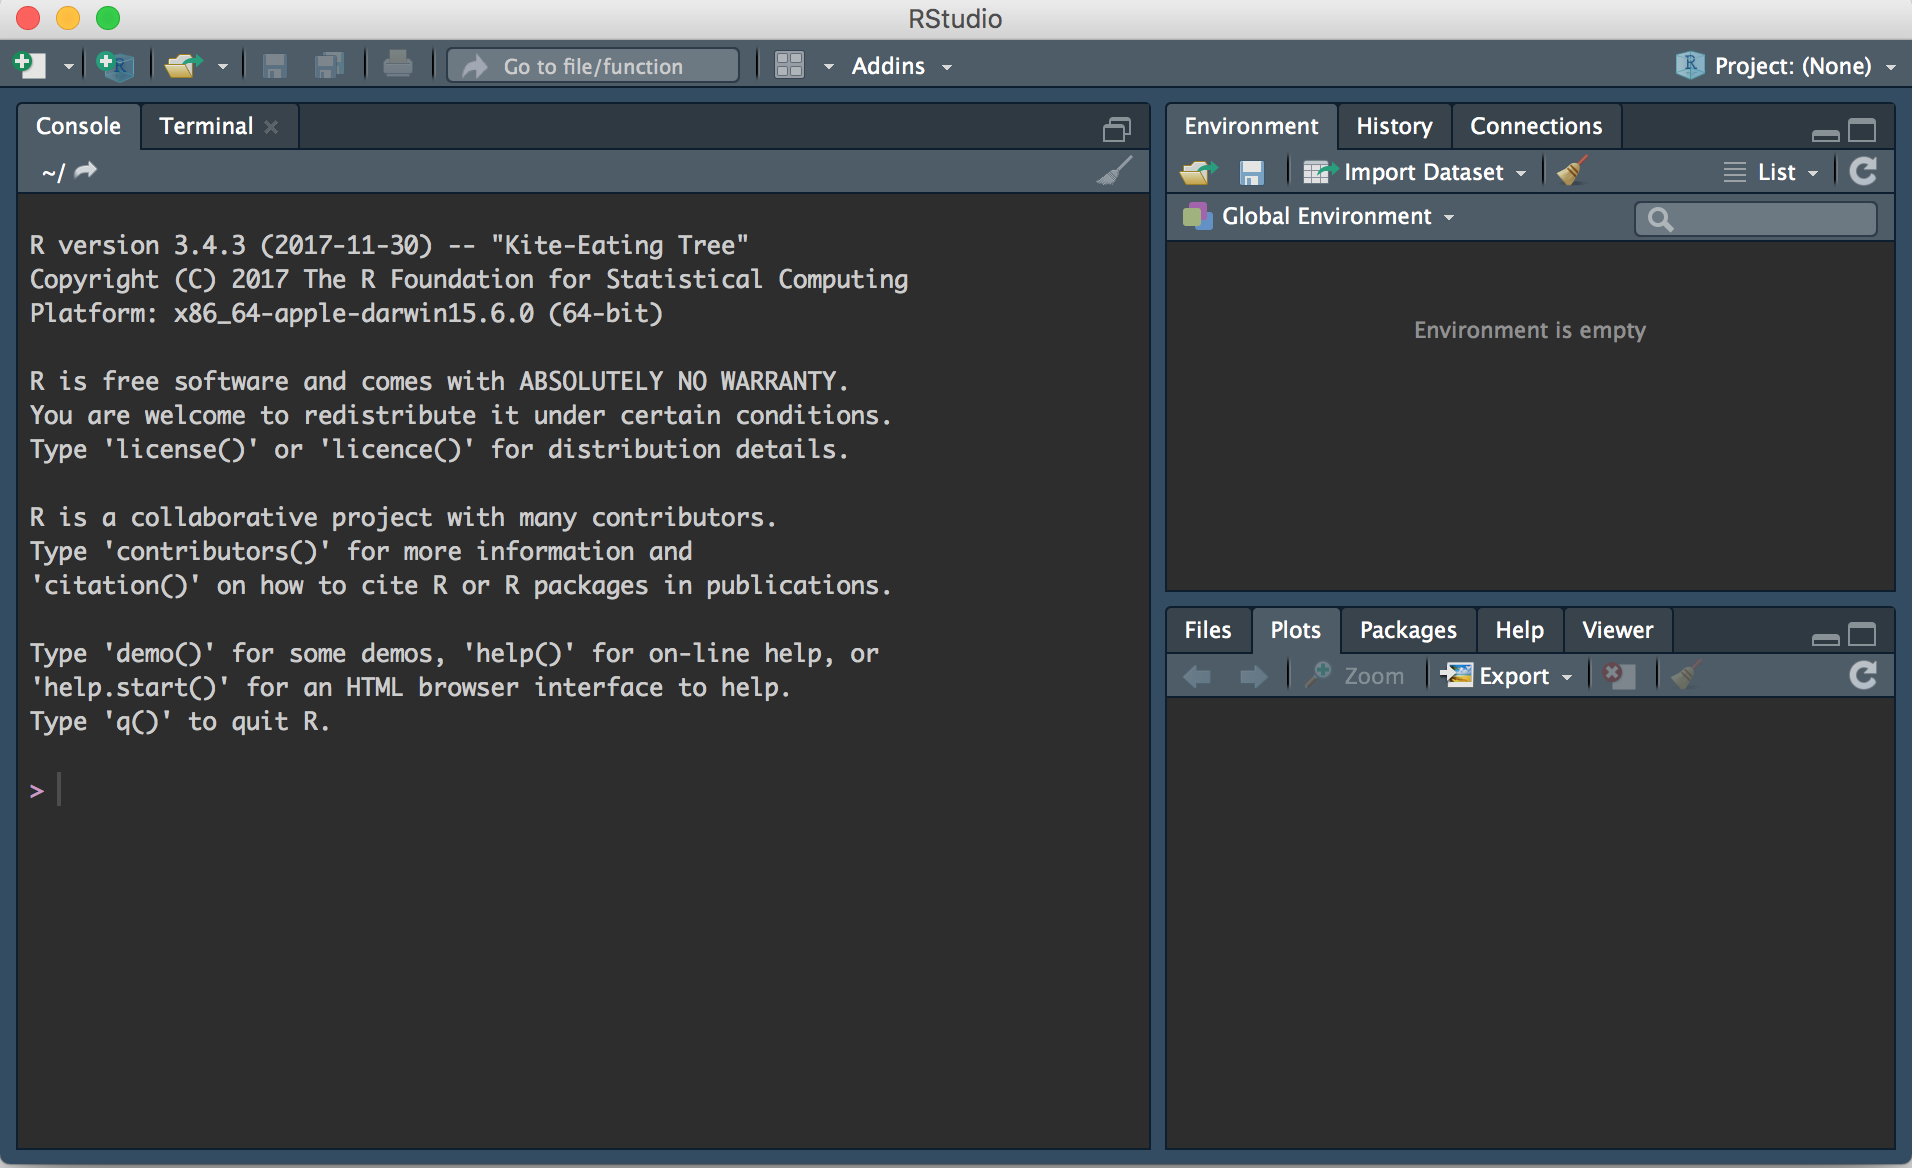
\includegraphics[width=1\linewidth]{fig/rstudio} \caption{Graphical interface in RStudio}\label{fig:interface}
  \end{figure}
  There are three different windows. However, one is missing, and that is
  the window where you will write most of your scripts. You can get this
  window by going to the top menu and select \texttt{File} \(\rightarrow\)
  \texttt{New\ File} \(\rightarrow\) \texttt{R\ Script}. This should give
  you four windows as shown in Figure \ref{fig:interfaceexplain}.
  \begin{figure}
  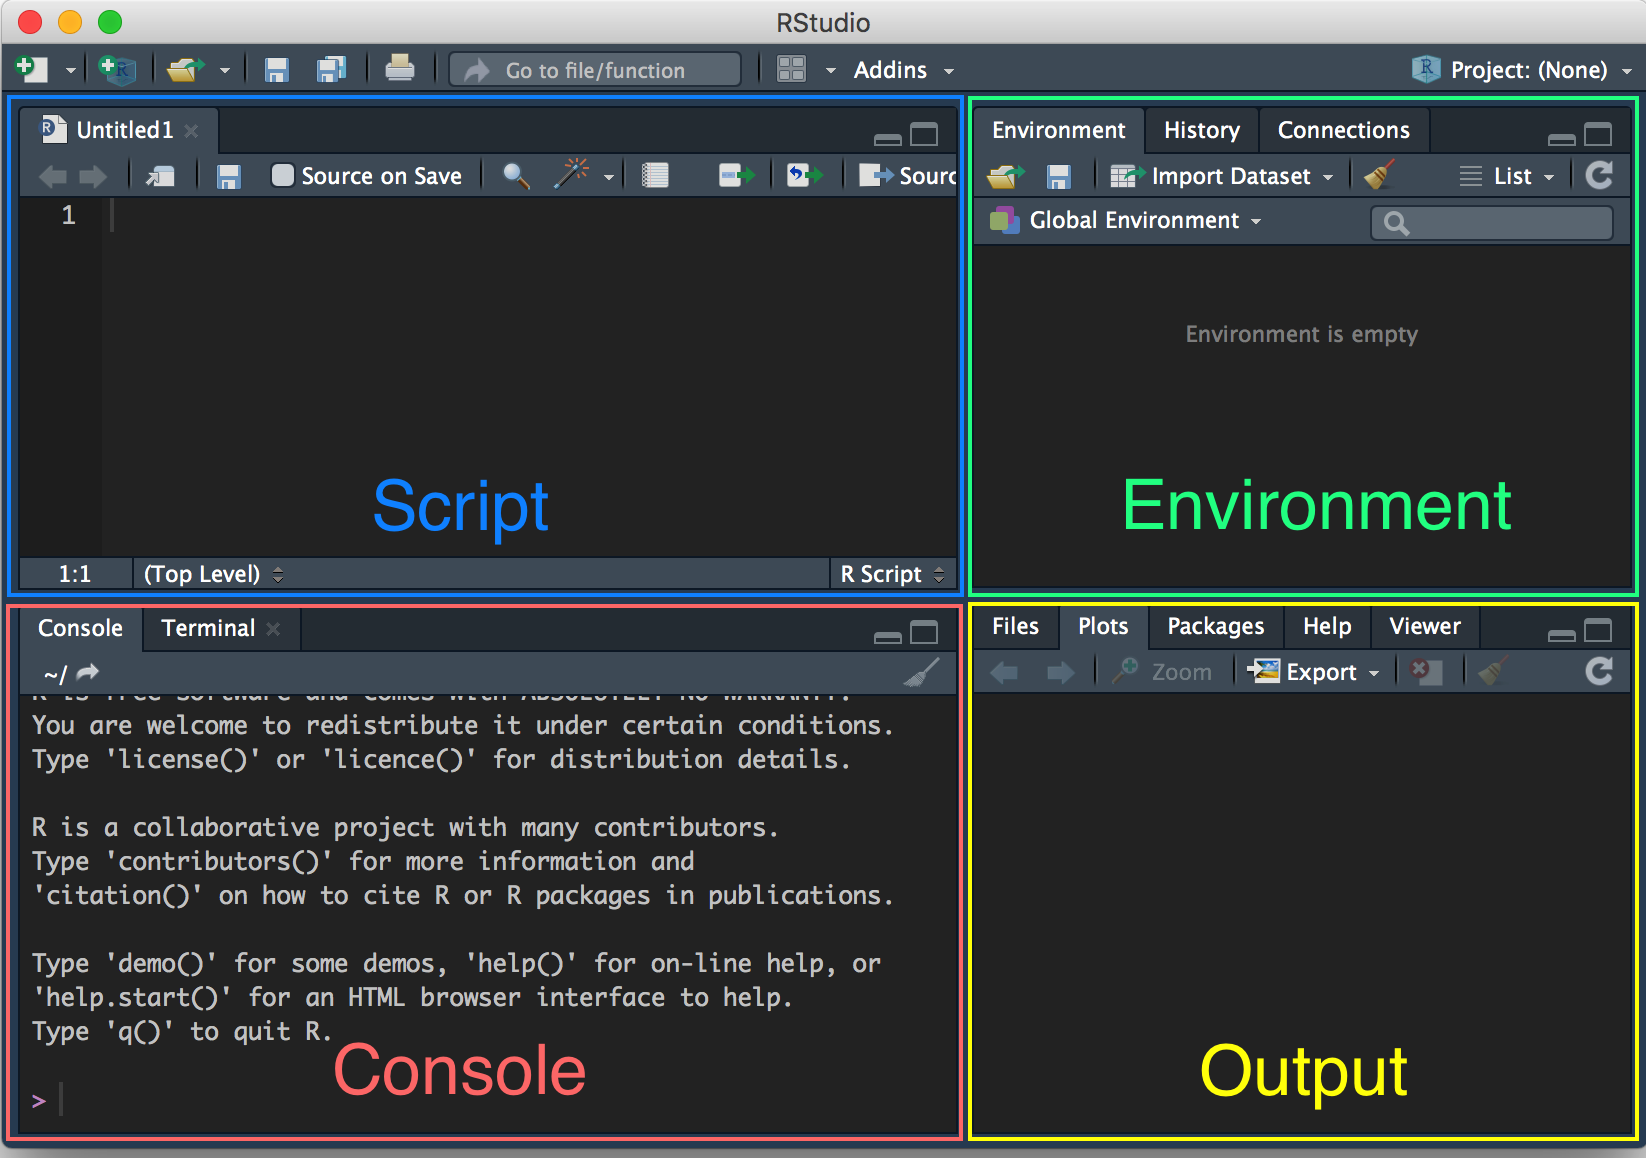
\includegraphics[width=1\linewidth]{fig/rstudio_env} \caption{Graphical interface in RStudio, explained}\label{fig:interfaceexplain}
  \end{figure}
  In the figure, we have emphasized the four windows: script, environment,
  output, and console. The \emph{script} is where you will have your
  \texttt{R} code and can add code and make changes to your script. The
  \emph{environment} is where you can see what datasets, variables and
  other parts you have loaded into \texttt{R}. The \emph{output} is where
  you can see the figures you create as well as documents. The
  \emph{console} is where you can see your output and run commands.
  
  Importantly, everything you do in \texttt{R} can be written as commands.
  This ensures that you will always be able to document your work (in the
  \texttt{script} window). In the console, you can see a prompt
  (\texttt{\textgreater{}}). Here, you can write what what you want
  \texttt{R} to do. Try to write \texttt{2+2} and hit \texttt{Enter}. This
  should look like the following:
  \begin{Shaded}
  \begin{Highlighting}[]
  \DecValTok{2}\OperatorTok{+}\DecValTok{2}
  \end{Highlighting}
  \end{Shaded}
  \begin{verbatim}
  [1] 4
  \end{verbatim}
  The code you have entered in the console cannot be traced later.
  Accordingly, you will have to save the commands you want to keep in the
  script. Even better, you should write your commands in the script and
  ``run'' them from there. If you write \texttt{2+2} in the script, you
  can mark it and press \texttt{CTRL+R} (Windows) or \texttt{CMD+ENTER}
  (Mac). Then it will run the part of the script you have marked. Insert
  the code below in your script, mark it, run it and see how the output
  shows up in the console:
  \begin{Shaded}
  \begin{Highlighting}[]
  \DecValTok{50}\OperatorTok{*}\DecValTok{149}
  \DecValTok{3}\OperatorTok{**}\DecValTok{2}        \CommentTok{# 3^2}
  \DecValTok{2}\OperatorTok{**}\DecValTok{3}        \CommentTok{# 2^3}
  \KeywordTok{sqrt}\NormalTok{(}\DecValTok{81}\NormalTok{)    }\CommentTok{# 81^0.5}
  \end{Highlighting}
  \end{Shaded}
  As you can see, we have used \texttt{\#} as well. The \texttt{\#} sign
  tells \texttt{R} that everything after that sign on that line shouldn't
  be read as code but as a comment. In other words, you can write comments
  in your script that will help you remember what you are doing - and help
  others understand the meaning of your script. For now, remember to
  document everything you do in your script.
  
  Notice also that we use a function in the bottom, namely
  \texttt{sqrt()}. A lot of what we will be doing in \texttt{R} works via
  functions. For example, to calculate a mean later we will use the
  \texttt{mean()} function. In the next section we will use functions to
  install and load packages.
  
  \section{\texorpdfstring{Installing \texttt{R}
  packages}{Installing R packages}}\label{installing-r-packages}
  
  We highlighted that one of the key advantages of using \texttt{R} is the
  package system. In \texttt{R}, a package is a collection of data and
  functions that makes it easier for you to do what you want. The sky is
  the limit and the only thing you need to learn now is how to install and
  load packages.
  
  To install packages, you will have to use a function called
  \texttt{install.packages()}. We will install a package that installs a
  lot of the functions we will be using to manipulate and visualise data.
  More specifically, we will work within the tidyverse (Hadley Wickham,
  2017). You can read more at \href{http://tidyverse.org/}{tidyverse.org}.
  To intall this package type:
  \begin{Shaded}
  \begin{Highlighting}[]
  \KeywordTok{install.packages}\NormalTok{(}\StringTok{"tidyverse"}\NormalTok{)}
  \end{Highlighting}
  \end{Shaded}
  You only need to install the package once. In other words, when you have
  used \texttt{install.packages()} to install a packagae, you will not
  need to install that specific package again. Note that we put
  \texttt{tidyverse} in quotation marks. This is important when you
  install a package. If you forget this, you will get an error.
  
  While you only need to install a package once, you need to load the
  package every time you open \texttt{R}. This is a good thing as you
  don't want to have all your installed \texttt{R} packages working at the
  same time if you don't need them. For this reason, most scripts begin
  with loading the packages that you need. To load a package, we use the
  function \texttt{library()}:
  \begin{Shaded}
  \begin{Highlighting}[]
  \KeywordTok{library}\NormalTok{(}\StringTok{"tidyverse"}\NormalTok{)}
  \end{Highlighting}
  \end{Shaded}
  To recap, it is always a good idea to begin your script with the
  package(s) you will be working with. If we want to have a script where
  we load the \texttt{tidyverse} package and have some of the commands we
  ran above, the script could look like the script presented in Figure
  \ref{fig:interfacescript}.
  \begin{figure}
  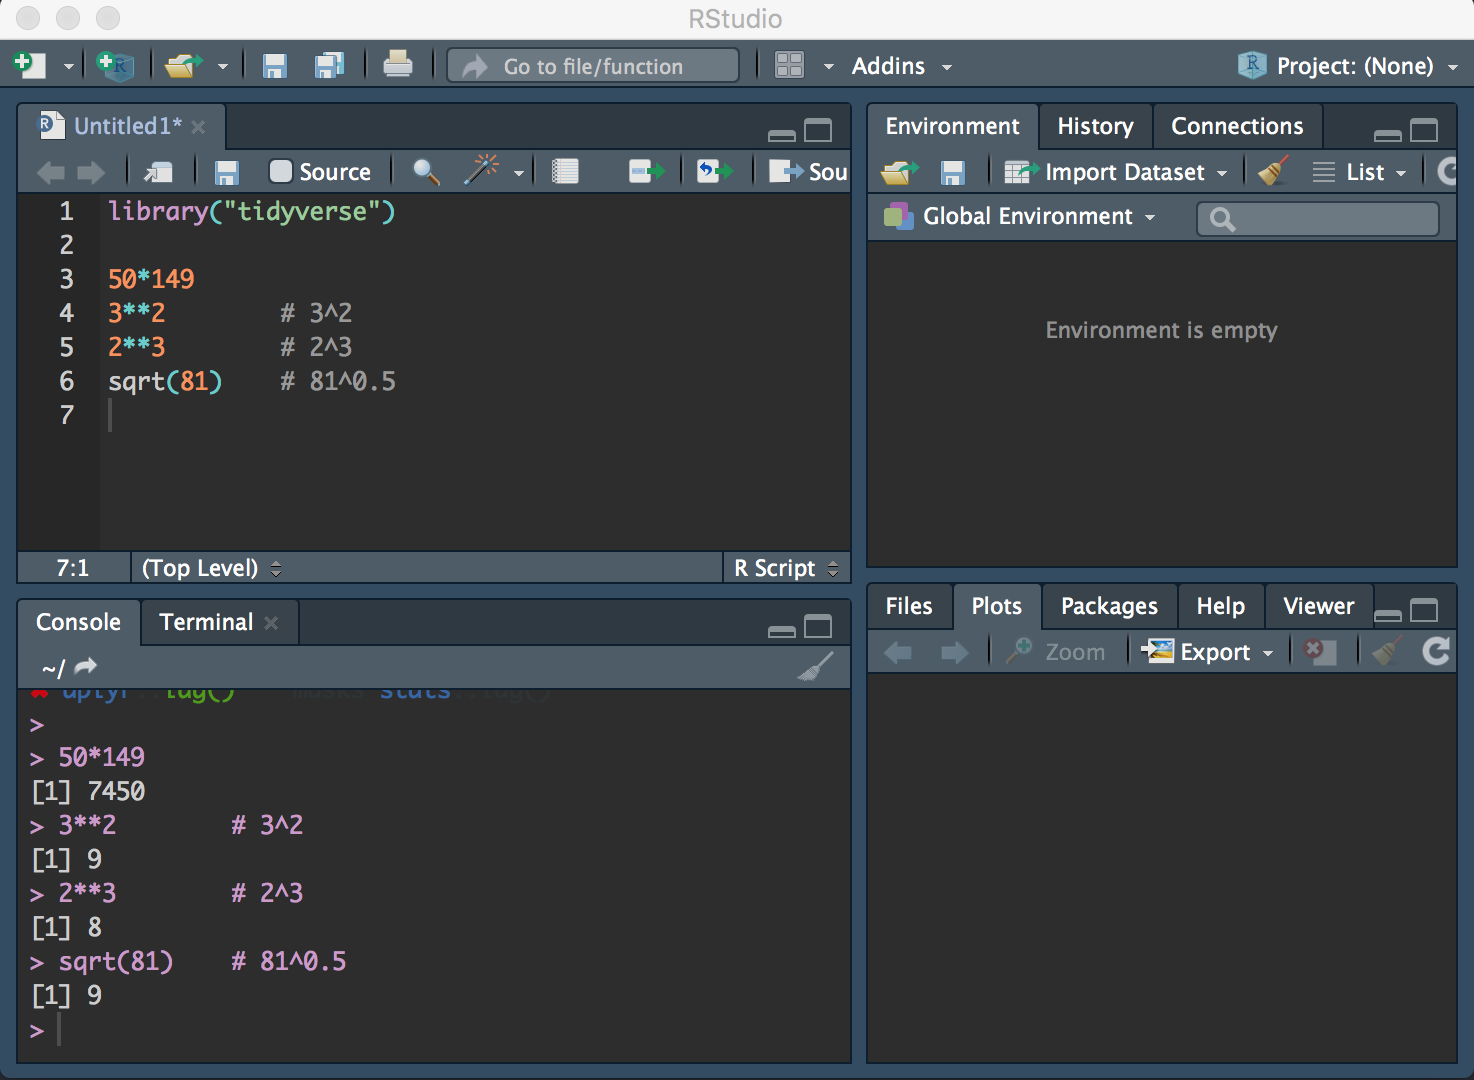
\includegraphics[width=1\linewidth]{fig/rstudio_script} \caption{A script in RStudio}\label{fig:interfacescript}
  \end{figure}
  If you want to save your script you can select \texttt{File}
  \(\rightarrow\) \texttt{Save}, where you can pick a destination for your
  script.
  
  \section{Errors and help}\label{errors-and-help}
  
  As noted above, you will encounter problems and issues when you do stuff
  in \texttt{R}. Sadly, there are many potential reasons to why your
  script might not be working. Your version of \texttt{R} or/and RStudio
  might be too old or too new, you might be using a function that has a
  mistake, you might not have the data in the right format etc.
  
  Consequently, we cannot provide a comprehensive list of errors you might
  get. The best thing to do is to learn how to find help online. Here, the
  best advice is to use Google and, when you search for help, always
  remember to mention R in your search string, and, if you are having
  problems with a specific package, also the name of the package.
  
  \chapter{Basics}\label{basics}
  
  Remember that everything you do in \texttt{R} can be written as
  commands. Repeat what you did in the last chapter from your script
  window: write \texttt{2+2} and run the code. This should look like the
  output below.
  \begin{Shaded}
  \begin{Highlighting}[]
  \DecValTok{2}\OperatorTok{+}\DecValTok{2}
  \end{Highlighting}
  \end{Shaded}
  \begin{verbatim}
  [1] 4
  \end{verbatim}
  You are now able to conduct simple arithmetics. This shows that
  \texttt{R} can be used as a calculatur and you can now call yourself an
  \texttt{R} user. In other words, knowing how to use \texttt{R} is not a
  binary category where you either can use \texttt{R} or not, but a
  continuum where you will always be able to learn more. That's great
  news!
  
  \section{Numbers as data}\label{numbers-as-data}
  
  Next, we will have to learn about variable assignment and in particular
  how we can work with \emph{objects}. Everything you will use in
  \texttt{R} is saved in objects. This can be everything from a number or
  a word to complex datasets. A key advantage of this, compared to other
  statistical programmes, is that you can have multiple datasets open at
  the same time. If you, for example, want to connect two different
  surveys, you can have them both loaded in the memory at the same time
  and work with them. This is not possible in SPSS or Stata.
  
  To save something in an object, we need to use the \emph{assignment
  operator}, \texttt{\textless{}-}, which basically tells \texttt{R} that
  anything on the right side of the operator should be assigned to the
  object on the left side. Let us try to save the number 2 in the object
  \texttt{x}.
  \begin{Shaded}
  \begin{Highlighting}[]
  \NormalTok{x <-}\StringTok{ }\DecValTok{2}
  \end{Highlighting}
  \end{Shaded}
  Now \texttt{x} will return the number 2 whenever we use \texttt{x}. Let
  us try to use our object in different simple operations. Write the
  operations below in your \texttt{R}-script and run them individually and
  see what happens.
  \begin{Shaded}
  \begin{Highlighting}[]
  \NormalTok{x}
  \NormalTok{x }\OperatorTok{*}\StringTok{ }\DecValTok{2}
  \NormalTok{x }\OperatorTok{*}\StringTok{ }\NormalTok{x }
  \NormalTok{x }\OperatorTok{+}\StringTok{ }\NormalTok{x}
  \end{Highlighting}
  \end{Shaded}
  If it is working, \texttt{R} should return the values \texttt{2},
  \texttt{4}, \texttt{4} and \texttt{4}. If you change the object
  \texttt{x} to have the number 3 instead of 2 and run the script again,
  you should get a new output.\footnote{More specifically, \texttt{3},
    \texttt{6}, \texttt{9} and \texttt{6}.} This is great as you only need
  to change a single number to change the output from the whole procedure.
  Accordingly, when you are working with scripts, try to save as much you
  can in objects, so you only need to change numbers once, if you want to
  make changes. This also reduces the likelihood of making mistakes.
  
  We can also use our object to create other objects. In the example below
  we will create a new object \texttt{y}. This object returns the sum of
  \texttt{x} and 7.
  \begin{Shaded}
  \begin{Highlighting}[]
  \NormalTok{y <-}\StringTok{ }\NormalTok{x }\OperatorTok{+}\StringTok{ }\DecValTok{7}
  \end{Highlighting}
  \end{Shaded}
  One thing to keep in mind is that we do not get the output in \texttt{y}
  right away. To get the output, we can just write \texttt{y}.
  \begin{Shaded}
  \begin{Highlighting}[]
  \NormalTok{y}
  \end{Highlighting}
  \end{Shaded}
  \begin{verbatim}
  [1] 9
  \end{verbatim}
  Alternatively, when we create the object, we can include it all in a
  parenthesis as we do below.
  \begin{Shaded}
  \begin{Highlighting}[]
  \NormalTok{(y <-}\StringTok{ }\NormalTok{x }\OperatorTok{+}\StringTok{ }\DecValTok{7}\NormalTok{)}
  \end{Highlighting}
  \end{Shaded}
  \begin{verbatim}
  [1] 9
  \end{verbatim}
  Luckily, we are not limited to save only one number in an object. On the
  contrary, in most objects we will be working with, we will have multiple
  numbers. The code below will return a row of numbers from 1 to 10.
  \begin{Shaded}
  \begin{Highlighting}[]
  \DecValTok{1}\OperatorTok{:}\DecValTok{10}
  \end{Highlighting}
  \end{Shaded}
  \begin{verbatim}
   [1]  1  2  3  4  5  6  7  8  9 10
  \end{verbatim}
  We can save this row of numbers in an object (again using
  \texttt{\textless{}-}), but we can also work with them directly, e.g.~by
  taking every number in the row and add 2 to all of them.
  \begin{Shaded}
  \begin{Highlighting}[]
  \DecValTok{1}\OperatorTok{:}\DecValTok{10} \OperatorTok{+}\StringTok{ }\DecValTok{2}
  \end{Highlighting}
  \end{Shaded}
  \begin{verbatim}
   [1]  3  4  5  6  7  8  9 10 11 12
  \end{verbatim}
  When you will be working with more numbers, you have to tell \texttt{R}
  that you are working with multiple numbers. To do this, we use the
  function \texttt{c()}. This tells \texttt{R} that we are working with a
  vector.\footnote{In the example with \texttt{1:10}, this is similar to
    writing \texttt{c(1,\ 2,\ 3,\ 4,\ 5,\ 6,\ 7,\ 8,\ 9,\ 10)} and
    \texttt{c(1:10)}. In other words, we have a hidden \texttt{c()} when
    we type \texttt{1:10}.} The function \texttt{c()} is short for
  \emph{concatenate} or \emph{combine}.\footnote{\texttt{c()} creates a
    vector with \emph{all} elements in the parenthesis. Since a vector can
    only have one type of data, and not both numbers and text (cf.~next
    section), \texttt{c()} will ensure that all values are reduced to the
    level all values can work with. Consequently, if just one value is a
    letter and not a number, all values in the vector will be considered
    text.} Remember that everything happening in \texttt{R} happens with
  functions. A vector can look like this:
  \begin{Shaded}
  \begin{Highlighting}[]
  \KeywordTok{c}\NormalTok{(}\DecValTok{2}\NormalTok{, }\DecValTok{2}\NormalTok{, }\DecValTok{2}\NormalTok{)}
  \end{Highlighting}
  \end{Shaded}
  \begin{verbatim}
  [1] 2 2 2
  \end{verbatim}
  This is a \emph{numerical} vector. A vector is a collection of values of
  the same type. We can save any vector in an object. In the code below we
  save four numbers (14, 6, 23, 2) in the object \texttt{x}.
  \begin{Shaded}
  \begin{Highlighting}[]
  \NormalTok{x <-}\StringTok{ }\KeywordTok{c}\NormalTok{(}\DecValTok{14}\NormalTok{, }\DecValTok{6}\NormalTok{, }\DecValTok{23}\NormalTok{, }\DecValTok{2}\NormalTok{)}
  \NormalTok{x}
  \end{Highlighting}
  \end{Shaded}
  \begin{verbatim}
  [1] 14  6 23  2
  \end{verbatim}
  We can then use this vector to calculate new numbers (just as we did
  above with \texttt{1:10}), for example by multiplying all the numbers in
  the vector with 2.
  \begin{Shaded}
  \begin{Highlighting}[]
  \NormalTok{x }\OperatorTok{*}\StringTok{ }\DecValTok{2}
  \end{Highlighting}
  \end{Shaded}
  \begin{verbatim}
  [1] 28 12 46  4
  \end{verbatim}
  If we are only interested in a single value from the vector, we can get
  this value by using brackets, i.e. \texttt{{[}\ {]}}, which you place
  just after the object (so no space between the name of the object and
  the brackets!). By placing the number 3 in the brackets we get the third
  number in the object.
  \begin{Shaded}
  \begin{Highlighting}[]
  \NormalTok{x[}\DecValTok{3}\NormalTok{]}
  \end{Highlighting}
  \end{Shaded}
  \begin{verbatim}
  [1] 23
  \end{verbatim}
  As you can see, we get the third element, 23. We can use the same
  procedure to get all values with the exception of one value by including
  a negative sign in the brackets. In the example below we will get all
  values except for 2. Also, note that since we are not assigning anything
  to an object (with \texttt{\textless{}-}), we are not making any changes
  to \texttt{x}.
  \begin{Shaded}
  \begin{Highlighting}[]
  \NormalTok{x[}\OperatorTok{-}\DecValTok{2}\NormalTok{]}
  \end{Highlighting}
  \end{Shaded}
  \begin{verbatim}
  [1] 14 23  2
  \end{verbatim}
  Now we can try to use a series of functions on our object. The functions
  below will return different types of information such as the median, the
  mean, the standard deviation etc.
  \begin{Shaded}
  \begin{Highlighting}[]
  \KeywordTok{length}\NormalTok{(x)     }\CommentTok{# length of vector, number of values}
  \KeywordTok{min}\NormalTok{(x)        }\CommentTok{# minima value}
  \KeywordTok{max}\NormalTok{(x)        }\CommentTok{# maxima value}
  \KeywordTok{median}\NormalTok{(x)     }\CommentTok{# the median}
  \KeywordTok{sum}\NormalTok{(x)        }\CommentTok{# the sum}
  \KeywordTok{mean}\NormalTok{(x)       }\CommentTok{# the mean}
  \KeywordTok{var}\NormalTok{(x)        }\CommentTok{# the variance}
  \KeywordTok{sd}\NormalTok{(x)         }\CommentTok{# the standard deviation}
  \end{Highlighting}
  \end{Shaded}
  The functions should return the values 4, 2, 23, 10, 45, 11.25, 86.25
  and 9.287088.
  
  If we for some reason wants to add an extra number to our vector
  \texttt{x}, we can either create a new vector with all the numbers or
  just overwrite the existing vector with the addition of an extra number:
  \begin{Shaded}
  \begin{Highlighting}[]
  \NormalTok{x <-}\StringTok{ }\KeywordTok{c}\NormalTok{(x, }\DecValTok{5}\NormalTok{)}
  \NormalTok{x}
  \end{Highlighting}
  \end{Shaded}
  \begin{verbatim}
  [1] 14  6 23  2  5
  \end{verbatim}
  We now have five values in our vector instead of four. The value 5 has
  the last place in the vector but if we had added 5 before \texttt{x} in
  the code above, 5 would have been in the beginning of the vector.
  
  Try to use the \texttt{mean()} function on the new object \texttt{x}
  \begin{Shaded}
  \begin{Highlighting}[]
  \KeywordTok{mean}\NormalTok{(x)}
  \end{Highlighting}
  \end{Shaded}
  \begin{verbatim}
  [1] 10
  \end{verbatim}
  Now the mean is 10 (before we added the value 5 to the object the mean
  was 11.25).
  
  \section{\texorpdfstring{Missing values
  (\texttt{NA})}{Missing values (NA)}}\label{missing-values-na}
  
  Up until now we have been lucky that all of our ``data'' has been easy
  to work with. However, in the real world - and thereby for most of the
  data we will work with - we will encounter missing values. In Stata you
  will see that missing values get a dot (`.'). In \texttt{R}, all missing
  values are denoted \texttt{NA}. Let us try to add a missing value to our
  object \texttt{x} and take the mean.
  \begin{Shaded}
  \begin{Highlighting}[]
  \NormalTok{x <-}\StringTok{ }\KeywordTok{c}\NormalTok{(x, }\OtherTok{NA}\NormalTok{)}
  
  \KeywordTok{mean}\NormalTok{(x) }
  \end{Highlighting}
  \end{Shaded}
  \begin{verbatim}
  [1] NA
  \end{verbatim}
  We do not get a mean now but just \texttt{NA}. The reason for this is
  that \texttt{R} is unable to calculate the mean of a vector with a
  missing value included. In order for \texttt{R} to calculate the mean
  now, we need to specify that it should remove the missing values before
  calculating the mean. To do this, we add \texttt{na.rm=TRUE} as an
  \emph{option} to the function. Most functions have a series of options
  (more on this later), and the default option for the \texttt{mean()}
  function is not to ignore the missing values.
  \begin{Shaded}
  \begin{Highlighting}[]
  \KeywordTok{mean}\NormalTok{(x, }\DataTypeTok{na.rm=}\OtherTok{TRUE}\NormalTok{)}
  \end{Highlighting}
  \end{Shaded}
  \begin{verbatim}
  [1] 10
  \end{verbatim}
  Now we get the same mean as before we added \texttt{NA} to the object.
  
  \section{Logical operators}\label{logical-operators}
  
  In \texttt{R} a lot of what we will be doing is using logical operators,
  e.g.~testing whether something is equal or similar to something else.
  This is in particular relevant when we have to recode objects and only
  use specific values. If something is true, we get the value
  \texttt{TRUE}, and if something is false, we get \texttt{FALSE}. Try to
  run the code below and see what information you get (and whether it
  makes sense).
  \begin{Shaded}
  \begin{Highlighting}[]
  \NormalTok{x <-}\StringTok{ }\DecValTok{2}
  
  \NormalTok{x }\OperatorTok{==}\StringTok{ }\DecValTok{2}        \CommentTok{# equal to}
  \NormalTok{x }\OperatorTok{==}\StringTok{ }\DecValTok{3}        
  \NormalTok{x }\OperatorTok{!=}\StringTok{ }\DecValTok{2}        \CommentTok{# not equal to}
  \NormalTok{x }\OperatorTok{<}\StringTok{ }\DecValTok{1}         \CommentTok{# less than}
  \NormalTok{x }\OperatorTok{>}\StringTok{ }\DecValTok{1}         \CommentTok{# greater than}
  \NormalTok{x }\OperatorTok{<=}\StringTok{ }\DecValTok{2}        \CommentTok{# less than or equal to}
  \NormalTok{x }\OperatorTok{>=}\StringTok{ }\FloatTok{2.01}     \CommentTok{# greater than or equal to}
  \end{Highlighting}
  \end{Shaded}
  The script will return \texttt{TRUE}, \texttt{FALSE}, \texttt{FALSE},
  \texttt{FALSE}, \texttt{TRUE}, \texttt{TRUE} and \texttt{FALSE}. If you
  change \texttt{x} to 3, the script will (logically) return other values.
  
  \section{Text as data}\label{text-as-data}
  
  In addition to numbers we can and will also work with text. The
  difference between text and numbers in \texttt{R} is that we use
  quotation marks to indicate that something is text (and not an
  object).\footnote{Alternatively, you can use ' instead of ``. If you
    want more information on when you should use ' instead of'', see
    \url{http://style.tidyverse.org/syntax.html\#quotes}.} As an example,
  we will create an object called \texttt{p} with the political parties
  from the United Kingdom general election in 2017.
  \begin{Shaded}
  \begin{Highlighting}[]
  \NormalTok{p <-}\StringTok{ }\KeywordTok{c}\NormalTok{(}\StringTok{"Conservative Party"}\NormalTok{, }\StringTok{"Labour Party"}\NormalTok{, }\StringTok{"Scottish National Party"}\NormalTok{, }
         \StringTok{"Liberal Democrats"}\NormalTok{, }\StringTok{"Democratic Unionist Party"}\NormalTok{, }\StringTok{"Sinn Féin"}\NormalTok{) }
  
  \NormalTok{p}
  \end{Highlighting}
  \end{Shaded}
  \begin{verbatim}
  [1] "Conservative Party"        "Labour Party"             
  [3] "Scottish National Party"   "Liberal Democrats"        
  [5] "Democratic Unionist Party" "Sinn Féin"                
  \end{verbatim}
  To see what type of data we have in our object, \texttt{p}, we can use
  the function \texttt{class()}. This function returns information on the
  type of data we are having in the object. If we use the function on
  \texttt{p}, we can see that the object consists of characters (i.e.
  \emph{``character''}).
  \begin{Shaded}
  \begin{Highlighting}[]
  \KeywordTok{class}\NormalTok{(p)}
  \end{Highlighting}
  \end{Shaded}
  \begin{verbatim}
  [1] "character"
  \end{verbatim}
  To compare, we can do the same thing with our object \texttt{x}, which
  includes numerical values. Here we see that the function
  \texttt{class()} for \texttt{x} returns \texttt{"numeric"}. The
  different classes a vector can have are: \texttt{character} (text),
  \texttt{numeric} (numbers), \texttt{integer} (whole numbers),
  \texttt{factor} (categories) and \texttt{logical} (logical).
  \begin{Shaded}
  \begin{Highlighting}[]
  \KeywordTok{class}\NormalTok{(x)}
  \end{Highlighting}
  \end{Shaded}
  \begin{verbatim}
  [1] "numeric"
  \end{verbatim}
  To test whether our object is numerical or not, we can use the function
  \texttt{is.numeric()}. If the object is numeric, we will get a
  \texttt{TRUE}. If not, we will get a \texttt{FALSE}. This logical
  structure can be used in a lot of different scenarios (as we will see
  later). Similar to \texttt{is.numeric()}, we have a function called
  \texttt{is.character()} that will show us whether the object is a
  charater or not.
  \begin{Shaded}
  \begin{Highlighting}[]
  \KeywordTok{is.numeric}\NormalTok{(x)}
  \KeywordTok{is.character}\NormalTok{(x)}
  \end{Highlighting}
  \end{Shaded}
  Try to use \texttt{is.numeric()} and \texttt{is.character()} on the
  object \texttt{p}.
  
  To get the number of characters for each element in our object, we can
  use the function \texttt{nchar()}:
  \begin{Shaded}
  \begin{Highlighting}[]
  \KeywordTok{nchar}\NormalTok{(p)}
  \end{Highlighting}
  \end{Shaded}
  \begin{verbatim}
  [1] 18 12 23 17 25  9
  \end{verbatim}
  We can also convert the characters in different ways. First, we can
  convert all characters to uppercase with \texttt{toupper()}. Second, we
  can concert all characters to lowercase with \texttt{tolower()}.
  \begin{Shaded}
  \begin{Highlighting}[]
  \KeywordTok{toupper}\NormalTok{(p)}
  \end{Highlighting}
  \end{Shaded}
  \begin{verbatim}
  [1] "CONSERVATIVE PARTY"        "LABOUR PARTY"             
  [3] "SCOTTISH NATIONAL PARTY"   "LIBERAL DEMOCRATS"        
  [5] "DEMOCRATIC UNIONIST PARTY" "SINN FÉIN"                
  \end{verbatim}
  \begin{Shaded}
  \begin{Highlighting}[]
  \KeywordTok{tolower}\NormalTok{(p) }
  \end{Highlighting}
  \end{Shaded}
  \begin{verbatim}
  [1] "conservative party"        "labour party"             
  [3] "scottish national party"   "liberal democrats"        
  [5] "democratic unionist party" "sinn féin"                
  \end{verbatim}
  In the same way we could get specific values from the object when it was
  numeric, we can get specific values when it is a character object as
  well.
  \begin{Shaded}
  \begin{Highlighting}[]
  \NormalTok{p[}\DecValTok{3}\NormalTok{]}
  \end{Highlighting}
  \end{Shaded}
  \begin{verbatim}
  [1] "Scottish National Party"
  \end{verbatim}
  \begin{Shaded}
  \begin{Highlighting}[]
  \NormalTok{p[}\OperatorTok{-}\DecValTok{3}\NormalTok{]}
  \end{Highlighting}
  \end{Shaded}
  \begin{verbatim}
  [1] "Conservative Party"        "Labour Party"             
  [3] "Liberal Democrats"         "Democratic Unionist Party"
  [5] "Sinn Féin"                
  \end{verbatim}
  While \texttt{p} is a short name for an object and easy to write, it is
  not telling for what we actually have stored in the object. Let us
  create a new object called \texttt{party} with the same information as
  in \texttt{p}. When you name objects remember that they are case
  sensitive so \texttt{party} will be a different object than
  \texttt{Party}.\footnote{If you want more information on how to name
    objects, see
    \url{http://style.tidyverse.org/syntax.html\#object-names}.}
  \begin{Shaded}
  \begin{Highlighting}[]
  \NormalTok{party <-}\StringTok{ }\NormalTok{p}
  
  \NormalTok{party}
  \end{Highlighting}
  \end{Shaded}
  \begin{verbatim}
  [1] "Conservative Party"        "Labour Party"             
  [3] "Scottish National Party"   "Liberal Democrats"        
  [5] "Democratic Unionist Party" "Sinn Féin"                
  \end{verbatim}
  \section{Data frames}\label{data-frames}
  
  In most cases, we will not be working with one variable
  (e.g.~information on party names) but multiple variables. To do this in
  an easy way, we can create \emph{data frames} which is similar to a
  dataset in SPSS and Stata. The good thing about \texttt{R}, however, is
  that we can have multiple data frames open at the same time. The cost of
  this is that we have to specify, when we do something in \texttt{R},
  exactly what data frame we are using.
  
  Here we will create a data frame with more information about the parties
  from the United Kingdom general election, 2017.\footnote{The information
    is taken from
    \url{https://en.wikipedia.org/wiki/United_Kingdom_general_election,_2017}}
  
  As a first step we can create new objects with more information:
  \texttt{leader} (information on the party leader), \texttt{votes} (the
  vote share in percent), \texttt{seats} (the number of seats) and
  \texttt{seats\_change} (change in seats from the previous election). Do
  note that the order is important as we are going to link these objects
  together in a minute, where the first value in each object is for the
  Conservative Party, the second for the Labour Party and so on.
  \begin{Shaded}
  \begin{Highlighting}[]
  \NormalTok{leader <-}\StringTok{ }\KeywordTok{c}\NormalTok{(}\StringTok{"Theresa May"}\NormalTok{, }\StringTok{"Jeremy Corbyn"}\NormalTok{, }\StringTok{"Nicola Sturgeon"}\NormalTok{, }
              \StringTok{"Tim Farron"}\NormalTok{, }\StringTok{"Arlene Foster"}\NormalTok{, }\StringTok{"Gerry Adams"}\NormalTok{)}
  \NormalTok{votes <-}\StringTok{ }\KeywordTok{c}\NormalTok{(}\FloatTok{42.4}\NormalTok{, }\FloatTok{40.0}\NormalTok{, }\FloatTok{3.0}\NormalTok{, }\FloatTok{7.4}\NormalTok{, }\FloatTok{0.9}\NormalTok{, }\FloatTok{0.7}\NormalTok{)}
  \NormalTok{seats <-}\StringTok{ }\KeywordTok{c}\NormalTok{(}\DecValTok{317}\NormalTok{, }\DecValTok{262}\NormalTok{, }\DecValTok{35}\NormalTok{, }\DecValTok{12}\NormalTok{, }\DecValTok{10}\NormalTok{, }\DecValTok{7}\NormalTok{)}
  \NormalTok{seats_change <-}\StringTok{ }\KeywordTok{c}\NormalTok{(}\OperatorTok{-}\DecValTok{13}\NormalTok{, }\DecValTok{30}\NormalTok{, }\OperatorTok{-}\DecValTok{21}\NormalTok{, }\DecValTok{4}\NormalTok{, }\DecValTok{2}\NormalTok{, }\DecValTok{3}\NormalTok{)}
  \end{Highlighting}
  \end{Shaded}
  The next thing we have to do is to connect the objects into a single
  object, i.e.~our data frame. A data frame is a collection of different
  vectors of the same length. In other words, for the objects we have
  above, as they have the same number of information, they can be
  connected in a data frame. \texttt{R} will return an error message if
  the vectors do not have the same length.
  
  We can have different types of variables in a data frame, i.e.~both
  numbers and text variables. To create our data frame, we will use the
  function \texttt{data.frame()} and save the data frame in the object
  \texttt{uk2017}.
  \begin{Shaded}
  \begin{Highlighting}[]
  \NormalTok{uk2017 <-}\StringTok{ }\KeywordTok{data.frame}\NormalTok{(party, leader, votes, seats, seats_change)}
  
  \NormalTok{uk2017 }\CommentTok{# show the content of the data frame}
  \end{Highlighting}
  \end{Shaded}
  \begin{verbatim}
                        party          leader votes seats seats_change
  1        Conservative Party     Theresa May  42.4   317          -13
  2              Labour Party   Jeremy Corbyn  40.0   262           30
  3   Scottish National Party Nicola Sturgeon   3.0    35          -21
  4         Liberal Democrats      Tim Farron   7.4    12            4
  5 Democratic Unionist Party   Arlene Foster   0.9    10            2
  6                 Sinn Féin     Gerry Adams   0.7     7            3
  \end{verbatim}
  To see what type of object we are working with, we can use the function
  \texttt{class()} again to show that \texttt{uk2017} is a data frame.
  \begin{Shaded}
  \begin{Highlighting}[]
  \KeywordTok{class}\NormalTok{(uk2017)}
  \end{Highlighting}
  \end{Shaded}
  \begin{verbatim}
  [1] "data.frame"
  \end{verbatim}
  If we would like to know what class the individual variables in our data
  frame are, we can use the function \texttt{sapply()}. This function
  allows us to apply a function to a list or a vector. Below we apply
  \texttt{class()} on the individual variables in \texttt{uk2017}.
  \begin{Shaded}
  \begin{Highlighting}[]
  \KeywordTok{sapply}\NormalTok{(uk2017, class)}
  \end{Highlighting}
  \end{Shaded}
  \begin{verbatim}
         party       leader        votes        seats seats_change 
      "factor"     "factor"    "numeric"    "numeric"    "numeric" 
  \end{verbatim}
  Here we can see that we have data as a \texttt{factor} as well as
  numerical variables. We can get similar information about our data by
  using the function \texttt{str()}. This function returns information on
  the structure of the data frame.
  \begin{Shaded}
  \begin{Highlighting}[]
  \KeywordTok{str}\NormalTok{(uk2017)}
  \end{Highlighting}
  \end{Shaded}
  \begin{verbatim}
  'data.frame':   6 obs. of  5 variables:
   $ party       : Factor w/ 6 levels "Conservative Party",..: 1 3 5 4 2 6
   $ leader      : Factor w/ 6 levels "Arlene Foster",..: 5 3 4 6 1 2
   $ votes       : num  42.4 40 3 7.4 0.9 0.7
   $ seats       : num  317 262 35 12 10 7
   $ seats_change: num  -13 30 -21 4 2 3
  \end{verbatim}
  We can see that it is a data frame with 6 observations of 5 variables.
  If the rows (i.e.~observations) have names, we can get these by using
  \texttt{rownames()}. We can get the names of the columns, i.e.~the
  variables in our data frame, by using \texttt{colnames()}.
  \begin{Shaded}
  \begin{Highlighting}[]
  \KeywordTok{colnames}\NormalTok{(uk2017)}
  \end{Highlighting}
  \end{Shaded}
  \begin{verbatim}
  [1] "party"        "leader"       "votes"        "seats"       
  [5] "seats_change"
  \end{verbatim}
  If we want to see the number of columns and rows in our data frame, we
  can use \texttt{ncol()} and \texttt{nrow()}.
  \begin{Shaded}
  \begin{Highlighting}[]
  \KeywordTok{ncol}\NormalTok{(uk2017)}
  \end{Highlighting}
  \end{Shaded}
  \begin{verbatim}
  [1] 5
  \end{verbatim}
  \begin{Shaded}
  \begin{Highlighting}[]
  \KeywordTok{nrow}\NormalTok{(uk2017)}
  \end{Highlighting}
  \end{Shaded}
  \begin{verbatim}
  [1] 6
  \end{verbatim}
  If we are working with bigger data frames, e.g.~a survey with thousands
  of respondents, it might not be useful to show the full data frame. One
  way to see a few of the observations is by using \texttt{head()}. If not
  specified further, this function will show the first six observations in
  the data frame. In the example below, we will tell \texttt{R} to show
  the first three observations
  \begin{Shaded}
  \begin{Highlighting}[]
  \KeywordTok{head}\NormalTok{(uk2017, }\DecValTok{3}\NormalTok{)  }\CommentTok{# show the first three rows}
  \end{Highlighting}
  \end{Shaded}
  \begin{verbatim}
                      party          leader votes seats seats_change
  1      Conservative Party     Theresa May  42.4   317          -13
  2            Labour Party   Jeremy Corbyn  40.0   262           30
  3 Scottish National Party Nicola Sturgeon   3.0    35          -21
  \end{verbatim}
  In the same way, we can use \texttt{tail()} to show the last
  observations in a data frame. Here we see the last four observations in
  our data frame.
  \begin{Shaded}
  \begin{Highlighting}[]
  \KeywordTok{tail}\NormalTok{(uk2017, }\DecValTok{4}\NormalTok{)  }\CommentTok{# show the last four rows}
  \end{Highlighting}
  \end{Shaded}
  \begin{verbatim}
                        party          leader votes seats seats_change
  3   Scottish National Party Nicola Sturgeon   3.0    35          -21
  4         Liberal Democrats      Tim Farron   7.4    12            4
  5 Democratic Unionist Party   Arlene Foster   0.9    10            2
  6                 Sinn Féin     Gerry Adams   0.7     7            3
  \end{verbatim}
  If you want to see your data frame in a new window, you can use the
  function \texttt{View()} (do note the capital letter V - not v).
  \begin{Shaded}
  \begin{Highlighting}[]
  \KeywordTok{View}\NormalTok{(uk2017)}
  \end{Highlighting}
  \end{Shaded}
  \begin{figure}
  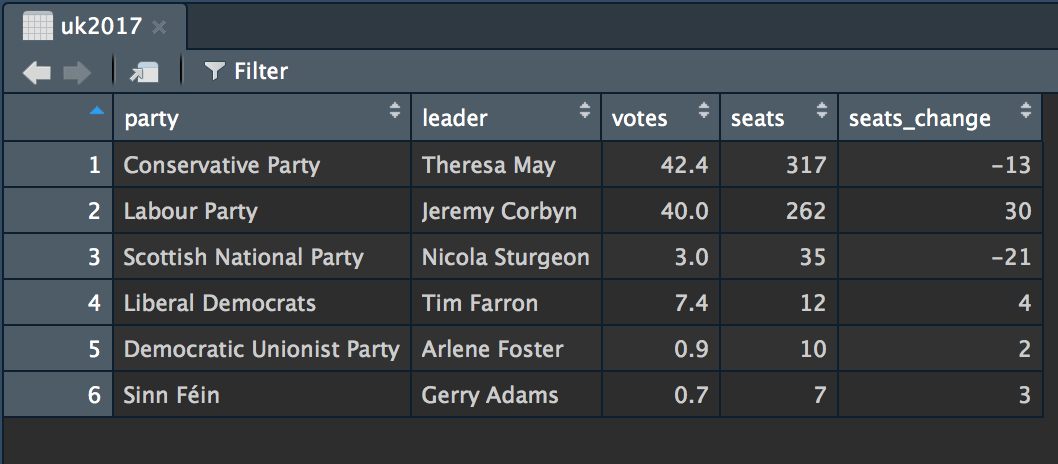
\includegraphics[width=14.69in,scale=0.65]{fig/View} \caption{Data frame with View(), RStudio}\label{fig:View}
  \end{figure}
  When you are working with variables in a data frame, you can use
  \texttt{\$} as a \emph{component selector} to select a variable in a
  data frame. This is the base R way, i.e.~brackets and dollar signs. In
  the next chapter we will work with other functions that makes it easier
  to work with data frames.
  
  If we, for example, want to have all the vote shares in our data frame
  \texttt{uk2017}, we can write \texttt{uk2017\$votes}.
  \begin{Shaded}
  \begin{Highlighting}[]
  \NormalTok{uk2017}\OperatorTok{$}\NormalTok{votes}
  \end{Highlighting}
  \end{Shaded}
  \begin{verbatim}
  [1] 42.4 40.0  3.0  7.4  0.9  0.7
  \end{verbatim}
  Contrary to working with a vector in a single dimension, we have two
  dimensions in a data frame (rows horisontally and columns vertically).
  Just as for a single vector, we need to work with the brackets,
  \texttt{{[}\ {]}}, in addition to our object. However, now we need to
  specify the rows \emph{and} columns we are interested in. If we want to
  work with the first row, we need to specify \texttt{{[}1,\ {]}} after
  the object. The comma is seperating the information on the rows and
  columns we want to work with. When we are not specifying anything after
  the comma, that means we want to have the information for \emph{all}
  columns.
  \begin{Shaded}
  \begin{Highlighting}[]
  \NormalTok{uk2017[}\DecValTok{1}\NormalTok{,] }\CommentTok{# first row}
  \end{Highlighting}
  \end{Shaded}
  \begin{verbatim}
                 party      leader votes seats seats_change
  1 Conservative Party Theresa May  42.4   317          -13
  \end{verbatim}
  Had we also added a number after the comma, we would get the information
  for that specific column. in the example below we want to have the
  information on the first row in the first column (i.e.~the name of the
  party on the first row).
  \begin{Shaded}
  \begin{Highlighting}[]
  \NormalTok{uk2017[}\DecValTok{1}\NormalTok{, }\DecValTok{1}\NormalTok{] }\CommentTok{# first row, first column}
  \end{Highlighting}
  \end{Shaded}
  \begin{verbatim}
  [1] Conservative Party
  6 Levels: Conservative Party Democratic Unionist Party ... Sinn Féin
  \end{verbatim}
  If we want to have the names of all parties, i.e.~the information in the
  first column, we can specify that we want all rows but only for the
  first column.
  \begin{Shaded}
  \begin{Highlighting}[]
  \NormalTok{uk2017[, }\DecValTok{1}\NormalTok{] }\CommentTok{# first column}
  \end{Highlighting}
  \end{Shaded}
  \begin{verbatim}
  [1] Conservative Party        Labour Party             
  [3] Scottish National Party   Liberal Democrats        
  [5] Democratic Unionist Party Sinn Féin                
  6 Levels: Conservative Party Democratic Unionist Party ... Sinn Féin
  \end{verbatim}
  Interestingly, the functions we have talked about so far can all be
  applied to data frames. The \texttt{summary()} function is very useful
  if you want to get an overview of all variables in your data frame. For
  the numerical variables in the data frame, the function will return
  information such as the mean and the median.
  \begin{Shaded}
  \begin{Highlighting}[]
  \KeywordTok{summary}\NormalTok{(uk2017)}
  \end{Highlighting}
  \end{Shaded}
  \begin{verbatim}
                         party               leader      votes       
   Conservative Party       :1   Arlene Foster  :1   Min.   : 0.700  
   Democratic Unionist Party:1   Gerry Adams    :1   1st Qu.: 1.425  
   Labour Party             :1   Jeremy Corbyn  :1   Median : 5.200  
   Liberal Democrats        :1   Nicola Sturgeon:1   Mean   :15.733  
   Scottish National Party  :1   Theresa May    :1   3rd Qu.:31.850  
   Sinn Féin                :1   Tim Farron     :1   Max.   :42.400  
       seats        seats_change     
   Min.   :  7.0   Min.   :-21.0000  
   1st Qu.: 10.5   1st Qu.: -9.2500  
   Median : 23.5   Median :  2.5000  
   Mean   :107.2   Mean   :  0.8333  
   3rd Qu.:205.2   3rd Qu.:  3.7500  
   Max.   :317.0   Max.   : 30.0000  
  \end{verbatim}
  We can also use the functions on our variables as we did above, e.g.~to
  get the maximum number of votes a party got with the function
  \texttt{max()}.
  \begin{Shaded}
  \begin{Highlighting}[]
  \KeywordTok{max}\NormalTok{(uk2017}\OperatorTok{$}\NormalTok{votes)}
  \end{Highlighting}
  \end{Shaded}
  \begin{verbatim}
  [1] 42.4
  \end{verbatim}
  If we want to have the value of a specific variable in our data frame,
  we can use both \texttt{\$} and \texttt{{[}\ {]}}. Below we get the
  second value in the variable \texttt{party}.
  \begin{Shaded}
  \begin{Highlighting}[]
  \NormalTok{uk2017}\OperatorTok{$}\NormalTok{party[}\DecValTok{2}\NormalTok{]}
  \end{Highlighting}
  \end{Shaded}
  \begin{verbatim}
  [1] Labour Party
  6 Levels: Conservative Party Democratic Unionist Party ... Sinn Féin
  \end{verbatim}
  To illustrate how we can combine a lot of what we have used above, we
  can get informatin on the name of the party that got the most votes. In
  order to do this, we specify that we would like to have the name of the
  party for the party where the number of votes equals the maximum number
  of votes. In other words, when \texttt{uk2017\$votes} is equal to
  \texttt{max(uk2017\$votes)}, we want to get the information on
  \texttt{uk2017\$party}. We use the logical operator \texttt{==} to test
  whether something is equal to.
  \begin{Shaded}
  \begin{Highlighting}[]
  \NormalTok{uk2017}\OperatorTok{$}\NormalTok{party[uk2017}\OperatorTok{$}\NormalTok{votes }\OperatorTok{==}\StringTok{ }\KeywordTok{max}\NormalTok{(uk2017}\OperatorTok{$}\NormalTok{votes)]}
  \end{Highlighting}
  \end{Shaded}
  \begin{verbatim}
  [1] Conservative Party
  6 Levels: Conservative Party Democratic Unionist Party ... Sinn Féin
  \end{verbatim}
  As we can see, the Conservative Party got the most votes in the 2017
  election. We can use the same procedure if we want to get information on
  the party that got the minimum number of votes. To do this we use
  \texttt{min()}. Here we can see that this is Sinn Féin in our data
  frame.
  \begin{Shaded}
  \begin{Highlighting}[]
  \NormalTok{uk2017}\OperatorTok{$}\NormalTok{party[uk2017}\OperatorTok{$}\NormalTok{votes }\OperatorTok{==}\StringTok{ }\KeywordTok{min}\NormalTok{(uk2017}\OperatorTok{$}\NormalTok{votes)]}
  \end{Highlighting}
  \end{Shaded}
  \begin{verbatim}
  [1] Sinn Féin
  6 Levels: Conservative Party Democratic Unionist Party ... Sinn Féin
  \end{verbatim}
  The sky is the limit when it comes to what we can do with data frames,
  including various types of statistical analyses. To give one example, we
  can use the \texttt{lm()} function to conduct an OLS regression with
  \texttt{votes} as the independent variable and \texttt{seats} as the
  dependent variable (more on this specific function in \texttt{R} later).
  First, we save the model in the object \texttt{uk2017\_lm} and then use
  \texttt{summary()} to get the results.
  \begin{Shaded}
  \begin{Highlighting}[]
  \NormalTok{uk2017_lm <-}\StringTok{ }\KeywordTok{lm}\NormalTok{(seats }\OperatorTok{~}\StringTok{ }\NormalTok{votes, }\DataTypeTok{data =}\NormalTok{ uk2017)}
  
  \KeywordTok{summary}\NormalTok{(uk2017_lm)}
  \end{Highlighting}
  \end{Shaded}
  \begin{verbatim}
  
  Call:
  lm(formula = seats ~ votes, data = uk2017)
  
  Residuals:
        1       2       3       4       5       6 
   20.890 -17.105  18.054 -36.122   7.933   6.350 
  
  Coefficients:
              Estimate Std. Error t value Pr(>|t|)    
  (Intercept)   -4.310     13.405  -0.321 0.763932    
  votes          7.085      0.558  12.698 0.000222 ***
  ---
  Signif. codes:  0 '***' 0.001 '**' 0.01 '*' 0.05 '.' 0.1 ' ' 1
  
  Residual standard error: 24.81 on 4 degrees of freedom
  Multiple R-squared:  0.9758,    Adjusted R-squared:  0.9697 
  F-statistic: 161.2 on 1 and 4 DF,  p-value: 0.0002216
  \end{verbatim}
  The coefficient for \texttt{votes} is positive and statistically
  significant (\(p<0.05\)). In other words, as the vote share increases,
  so does the number of seats.
  
  \section{Import and export data
  frames}\label{import-and-export-data-frames}
  
  Most of the data frames we will be working with in \texttt{R} are not
  data frames we will build from scratch but on the contrary data frames
  we will import from other files such as files made for Stata, SPSS or
  Excel. The most useful filetype to use when you work with data in files
  is \texttt{.csv}, which stands for \emph{comma-separated values}. This
  is an open file format and can be opened in any software. To export and
  import data frames to \texttt{.csv} files, we can use
  \texttt{write.csv()} and \texttt{read.csv()}.
  
  First of all we need to know where \texttt{R} is working from, i.e.~what
  our \emph{working directory} is. In other words, we need to tell
  \texttt{R} where it should be saving the file and - when we want to
  import a data frame - where to look for a file. To see where \texttt{R}
  is currently working from (the \emph{working directory}) you can type
  \texttt{getwd()}. This will return the place where \texttt{R} is
  currently going to save the file if we do not change it.
  \begin{Shaded}
  \begin{Highlighting}[]
  \KeywordTok{getwd}\NormalTok{()}
  \end{Highlighting}
  \end{Shaded}
  If you would like to change this, you can use the function
  \texttt{setwd()}. This function allows you to change the working
  directory to whatever folder on your computer you would like to use. In
  the code below I change the working directory to the folder
  \texttt{book} in the folder \texttt{qpolr} in the Dropbox folder. Do
  also note that we are using forward slash (\texttt{/}) and not backslash
  (\texttt{\textbackslash{}}).
  \begin{Shaded}
  \begin{Highlighting}[]
  \KeywordTok{setwd}\NormalTok{(}\StringTok{"/Dropbox/qpolr/book"}\NormalTok{)}
  \end{Highlighting}
  \end{Shaded}
  An easy way to control the working directory is to open an
  \texttt{R}-script directly from the folder you want to have as your
  working directory. Specifically, instead of opening RStudio and finding
  the script, find the script in your folder and open RStudio that way.
  This will automatically set the working directory to the folder with the
  \texttt{R}-script.
  
  Once we know where we will save our data, we can use
  \texttt{write.csv()} to save the data. In the code below we first
  specify that we want to save the data frame \texttt{uk2017} and next the
  filename of the file (\texttt{uk2017.csv}).
  \begin{Shaded}
  \begin{Highlighting}[]
  \KeywordTok{write.csv}\NormalTok{(uk2017, }\StringTok{"uk2017.csv"}\NormalTok{)}
  \end{Highlighting}
  \end{Shaded}
  Do note that we need to put the file in quotation marks. Next, we can
  import the file into \texttt{R} the next time we open \texttt{R} with
  the function \texttt{read.csv()} and save the data frame in the object
  \texttt{uk2017}.
  \begin{Shaded}
  \begin{Highlighting}[]
  \NormalTok{uk2017 <-}\StringTok{ }\KeywordTok{read.csv}\NormalTok{(}\StringTok{"uk2017.csv"}\NormalTok{)}
  \end{Highlighting}
  \end{Shaded}
  As with most stuff in \texttt{R}, there are multiple ways of doing
  things. To import and export data, we have packages like
  \texttt{foreign} (R Core Team, 2015), \texttt{rio} (C. Chan, Chan, \&
  Leeper, 2016) and \texttt{readr} (H. Wickham \& Francois, 2015). If you
  install and load the package \texttt{rio}, you can use the functions
  \texttt{import()} and \texttt{export()}.
  \begin{Shaded}
  \begin{Highlighting}[]
  \CommentTok{# export data with the rio package}
  \KeywordTok{export}\NormalTok{(uk2017, }\StringTok{"uk2017.csv"}\NormalTok{)}
  
  \CommentTok{# import data with the rio package}
  \NormalTok{uk2017 <-}\StringTok{ }\KeywordTok{import}\NormalTok{(}\StringTok{"uk2017.csv"}\NormalTok{)}
  \end{Highlighting}
  \end{Shaded}
  \section{Environment}\label{environment}
  
  We have worked with a series of different objects. To see what objects
  we have in our memory, we can look in the \emph{Environment} window, but
  we can also use the function \texttt{ls()}(\emph{ls} is short for
  \emph{list objects}).
  \begin{Shaded}
  \begin{Highlighting}[]
  \KeywordTok{ls}\NormalTok{()}
  \end{Highlighting}
  \end{Shaded}
  \begin{verbatim}
   [1] "leader"       "p"            "party"        "seats"       
   [5] "seats_change" "uk2017"       "uk2017_lm"    "votes"       
   [9] "x"            "y"           
  \end{verbatim}
  If we would like to remove an object from the memory, we can use the
  function \texttt{rm()} (\emph{rm} is short for \emph{remove}). Below we
  use \texttt{rm()} to remove the object \texttt{x} and then \texttt{ls()}
  to check whether \texttt{x} is gone.
  \begin{Shaded}
  \begin{Highlighting}[]
  \KeywordTok{rm}\NormalTok{(x)}
  
  \KeywordTok{ls}\NormalTok{()}
  \end{Highlighting}
  \end{Shaded}
  \begin{verbatim}
  [1] "leader"       "p"            "party"        "seats"       
  [5] "seats_change" "uk2017"       "uk2017_lm"    "votes"       
  [9] "y"           
  \end{verbatim}
  If you would like to remove \emph{everything} in the memory, you can use
  \texttt{ls()} in combination with \texttt{rm()}.
  \begin{Shaded}
  \begin{Highlighting}[]
  \KeywordTok{rm}\NormalTok{(}\DataTypeTok{list =} \KeywordTok{ls}\NormalTok{())}
  
  \KeywordTok{ls}\NormalTok{()}
  \end{Highlighting}
  \end{Shaded}
  \chapter*{(PART) Working with data}\label{part-working-with-data}
  \addcontentsline{toc}{chapter}{(PART) Working with data}
  
  \chapter{Data management}\label{data}
  
  There are multiple ways to manage data in \texttt{R} and in particular
  different ways to create and change variables in a data frame. In this
  chapter, we show different ways of working with data frames with a focus
  on how to change and create new variables. Noteworthy, there are
  multiple packages we can use to manipulate data frames, but the best is
  without a doubt \texttt{dplyr} (Hadley Wickham \& Francois, 2016). This
  is part of the \texttt{tidyverse} package so you do not need to install
  any new packages if you have already installed \texttt{tidyverse}.
  
  The package provides some basic functions making it easy to work with
  data frames. These functions include \texttt{select()},
  \texttt{filter()}, \texttt{arrange()}, \texttt{rename()},
  \texttt{mutate()} and \texttt{summarize()}.\footnote{For another good
    introduction to \texttt{dplyr}, see:
    \href{https://bookdown.org/rdpeng/rprogdatascience/managing-data-frames-with-the-dplyr-package.html}{Managing
    Data Frames with the dplyr package}.} \texttt{select()} allows you to
  pick variables by their names. \texttt{filter()} allows you to pick
  observations by their values. \texttt{arrange()} allows you to reorder
  the rows. \texttt{rename()} allows you to rename columns.
  \texttt{mutate()} allows you to create new variables based on the values
  of old variables. \texttt{summarize()} allows you to collapse many
  values to a single summary.
  
  All these functions rely on data frames. In other words, you can not use
  these functions on other types of data in \texttt{R}. Furthermore, they
  all return a new data frame that you will need to save in a new object
  or overwrite the existing object with your data frame.
  
  As the \texttt{dplyr} package is part of the \texttt{tidyverse}, the
  first thing we do is to call the \texttt{tidyverse}.
  \begin{Shaded}
  \begin{Highlighting}[]
  \KeywordTok{library}\NormalTok{(}\StringTok{"tidyverse"}\NormalTok{)}
  \end{Highlighting}
  \end{Shaded}
  We will use the dataset we created in the previous chapter. If you do
  not have it, you can download it here (make sure to have the data file
  saved in your working directory): \url{http://qpolr.com/data/uk2017.csv}
  \begin{Shaded}
  \begin{Highlighting}[]
  \NormalTok{uk2017 <-}\StringTok{ }\KeywordTok{read.csv}\NormalTok{(}\StringTok{"uk2017.csv"}\NormalTok{)}
  \end{Highlighting}
  \end{Shaded}
  To see the information in the dataset, use \texttt{head()}.
  \begin{Shaded}
  \begin{Highlighting}[]
  \KeywordTok{head}\NormalTok{(uk2017)}
  \end{Highlighting}
  \end{Shaded}
  \begin{verbatim}
                        party          leader votes seats seats_change
  1        Conservative Party     Theresa May  42.4   317          -13
  2              Labour Party   Jeremy Corbyn  40.0   262           30
  3   Scottish National Party Nicola Sturgeon   3.0    35          -21
  4         Liberal Democrats      Tim Farron   7.4    12            4
  5 Democratic Unionist Party   Arlene Foster   0.9    10            2
  6                 Sinn Féin     Gerry Adams   0.7     7            3
  \end{verbatim}
  \section{\texorpdfstring{Selecting variables:
  \texttt{select()}}{Selecting variables: select()}}\label{selecting-variables-select}
  
  When we work with large datasets, we often want to select the few
  variables that are of key interest to our project. For this task the
  \texttt{select()} function is perfect. If we only want to have
  information on the party name and the votes in the \texttt{uk2017} data
  frame, we can write:
  \begin{Shaded}
  \begin{Highlighting}[]
  \KeywordTok{select}\NormalTok{(uk2017, party, votes)}
  \end{Highlighting}
  \end{Shaded}
  \begin{verbatim}
                        party votes
  1        Conservative Party  42.4
  2              Labour Party  40.0
  3   Scottish National Party   3.0
  4         Liberal Democrats   7.4
  5 Democratic Unionist Party   0.9
  6                 Sinn Féin   0.7
  \end{verbatim}
  Again, this is not saved in a new data frame. If we want to save this in
  a new data frame, say \texttt{uk2017\_pv}, we need to assign the output
  from \texttt{select()} to our object.
  \begin{Shaded}
  \begin{Highlighting}[]
  \NormalTok{uk2017_pv <-}\StringTok{ }\KeywordTok{select}\NormalTok{(uk2017, party, votes)}
  \end{Highlighting}
  \end{Shaded}
  There are multiple different functions that can help us find specific
  variables in the data frame. We can use \texttt{contains()}, if we want
  to include variables that contain a specific word in the variable name.
  In the example below we look for variables that contain the text
  \texttt{seat}.
  \begin{Shaded}
  \begin{Highlighting}[]
  \KeywordTok{select}\NormalTok{(uk2017, }\KeywordTok{contains}\NormalTok{(}\StringTok{"seat"}\NormalTok{))}
  \end{Highlighting}
  \end{Shaded}
  \begin{verbatim}
    seats seats_change
  1   317          -13
  2   262           30
  3    35          -21
  4    12            4
  5    10            2
  6     7            3
  \end{verbatim}
  Other noteworthy functions similar to \texttt{contains()} that can be of
  help are functions such as \texttt{starts\_with()},
  \texttt{ends\_with()}, \texttt{matches()}, \texttt{num\_range()},
  \texttt{one\_of()} and \texttt{everything()}. The last function,
  \texttt{everything()} is helpful if we want to move a variable to the
  beginning of our data frame.
  \begin{Shaded}
  \begin{Highlighting}[]
  \KeywordTok{select}\NormalTok{(uk2017, votes, }\KeywordTok{everything}\NormalTok{())}
  \end{Highlighting}
  \end{Shaded}
  \begin{verbatim}
    votes                     party          leader seats seats_change
  1  42.4        Conservative Party     Theresa May   317          -13
  2  40.0              Labour Party   Jeremy Corbyn   262           30
  3   3.0   Scottish National Party Nicola Sturgeon    35          -21
  4   7.4         Liberal Democrats      Tim Farron    12            4
  5   0.9 Democratic Unionist Party   Arlene Foster    10            2
  6   0.7                 Sinn Féin     Gerry Adams     7            3
  \end{verbatim}
  Last, we can use the negative sign if we want to remove a variable from
  the data frame.
  \begin{Shaded}
  \begin{Highlighting}[]
  \KeywordTok{select}\NormalTok{(uk2017, }\OperatorTok{-}\NormalTok{leader)}
  \end{Highlighting}
  \end{Shaded}
  \begin{verbatim}
                        party votes seats seats_change
  1        Conservative Party  42.4   317          -13
  2              Labour Party  40.0   262           30
  3   Scottish National Party   3.0    35          -21
  4         Liberal Democrats   7.4    12            4
  5 Democratic Unionist Party   0.9    10            2
  6                 Sinn Féin   0.7     7            3
  \end{verbatim}
  \section{\texorpdfstring{Selecting observations:
  \texttt{filter()}}{Selecting observations: filter()}}\label{selecting-observations-filter}
  
  To select only some of the observations in our data frame, but for all
  variables, we can use the function \texttt{filter()}. In the example
  below we select the observations in our data frame with a positive value
  on \texttt{seats\_change} (i.e.~greater than 0).
  \begin{Shaded}
  \begin{Highlighting}[]
  \KeywordTok{filter}\NormalTok{(uk2017, seats_change }\OperatorTok{>}\StringTok{ }\DecValTok{0}\NormalTok{)}
  \end{Highlighting}
  \end{Shaded}
  \begin{verbatim}
  Warning: package 'bindrcpp' was built under R version 3.4.4
  \end{verbatim}
  \begin{verbatim}
                        party        leader votes seats seats_change
  1              Labour Party Jeremy Corbyn  40.0   262           30
  2         Liberal Democrats    Tim Farron   7.4    12            4
  3 Democratic Unionist Party Arlene Foster   0.9    10            2
  4                 Sinn Féin   Gerry Adams   0.7     7            3
  \end{verbatim}
  Importantly, we are \emph{not} making any changes to the data frame
  \texttt{uk2017}. Again, this will only hapen if we replace our existing
  data frame or create a new data frame. In the example below we create a
  new data frame, \texttt{uk2017\_seatlosers}, with the observations
  losing seats from 2015 to 2017.
  \begin{Shaded}
  \begin{Highlighting}[]
  \NormalTok{uk2017_seatlosers <-}\StringTok{ }\KeywordTok{filter}\NormalTok{(uk2017, seats_change }\OperatorTok{<}\StringTok{ }\DecValTok{0}\NormalTok{)}
  \NormalTok{uk2017_seatlosers}
  \end{Highlighting}
  \end{Shaded}
  \begin{verbatim}
                      party          leader votes seats seats_change
  1      Conservative Party     Theresa May  42.4   317          -13
  2 Scottish National Party Nicola Sturgeon   3.0    35          -21
  \end{verbatim}
  Last, if we want to drop observations that contain missing values on
  specific variables, we can use the function \texttt{drop\_na()}.
  
  \section{\texorpdfstring{Sorting observations:
  \texttt{arrange()}}{Sorting observations: arrange()}}\label{sorting-observations-arrange}
  
  We can use the function \texttt{arrange()} if we want to change the
  order of observations. In the example below we sort our data frame
  according to how many votes the party got, with the party getting the
  least votes in the top of our data frame.
  \begin{Shaded}
  \begin{Highlighting}[]
  \KeywordTok{arrange}\NormalTok{(uk2017, votes)}
  \end{Highlighting}
  \end{Shaded}
  \begin{verbatim}
                        party          leader votes seats seats_change
  1                 Sinn Féin     Gerry Adams   0.7     7            3
  2 Democratic Unionist Party   Arlene Foster   0.9    10            2
  3   Scottish National Party Nicola Sturgeon   3.0    35          -21
  4         Liberal Democrats      Tim Farron   7.4    12            4
  5              Labour Party   Jeremy Corbyn  40.0   262           30
  6        Conservative Party     Theresa May  42.4   317          -13
  \end{verbatim}
  If we prefer to have the parties with the greatest number of votes in
  the top, we can use the negative sign (\texttt{-}).
  \begin{Shaded}
  \begin{Highlighting}[]
  \KeywordTok{arrange}\NormalTok{(uk2017, }\OperatorTok{-}\NormalTok{votes)}
  \end{Highlighting}
  \end{Shaded}
  \begin{verbatim}
                        party          leader votes seats seats_change
  1        Conservative Party     Theresa May  42.4   317          -13
  2              Labour Party   Jeremy Corbyn  40.0   262           30
  3         Liberal Democrats      Tim Farron   7.4    12            4
  4   Scottish National Party Nicola Sturgeon   3.0    35          -21
  5 Democratic Unionist Party   Arlene Foster   0.9    10            2
  6                 Sinn Féin     Gerry Adams   0.7     7            3
  \end{verbatim}
  \section{\texorpdfstring{Rename variables:
  \texttt{rename()}}{Rename variables: rename()}}\label{rename-variables-rename}
  
  In the case that we have a variable we would prefer having another name,
  we can use the function \texttt{rename()}. In the example below we
  change the name of \texttt{party} to \texttt{party\_name}.
  \begin{Shaded}
  \begin{Highlighting}[]
  \KeywordTok{rename}\NormalTok{(uk2017, }\DataTypeTok{party_name =}\NormalTok{ party)}
  \end{Highlighting}
  \end{Shaded}
  \begin{verbatim}
                   party_name          leader votes seats seats_change
  1        Conservative Party     Theresa May  42.4   317          -13
  2              Labour Party   Jeremy Corbyn  40.0   262           30
  3   Scottish National Party Nicola Sturgeon   3.0    35          -21
  4         Liberal Democrats      Tim Farron   7.4    12            4
  5 Democratic Unionist Party   Arlene Foster   0.9    10            2
  6                 Sinn Féin     Gerry Adams   0.7     7            3
  \end{verbatim}
  \section{\texorpdfstring{Create variables:
  \texttt{mutate()}}{Create variables: mutate()}}\label{create-variables-mutate}
  
  The best way to create a new variable from existing variables in our
  data frame is to use the function \texttt{mutate()}. In the example
  below we create a new variable, \texttt{votes\_m} with information on
  how many percentage points a party is from the average number of votes a
  party got in the election.
  \begin{Shaded}
  \begin{Highlighting}[]
  \KeywordTok{mutate}\NormalTok{(uk2017, }\DataTypeTok{votes_m =}\NormalTok{ votes }\OperatorTok{-}\StringTok{ }\KeywordTok{mean}\NormalTok{(votes))}
  \end{Highlighting}
  \end{Shaded}
  \begin{verbatim}
                        party          leader votes seats seats_change
  1        Conservative Party     Theresa May  42.4   317          -13
  2              Labour Party   Jeremy Corbyn  40.0   262           30
  3   Scottish National Party Nicola Sturgeon   3.0    35          -21
  4         Liberal Democrats      Tim Farron   7.4    12            4
  5 Democratic Unionist Party   Arlene Foster   0.9    10            2
  6                 Sinn Féin     Gerry Adams   0.7     7            3
       votes_m
  1  26.666667
  2  24.266667
  3 -12.733333
  4  -8.333333
  5 -14.833333
  6 -15.033333
  \end{verbatim}
  We can also use the \texttt{sum()} function to find the proportion of
  seats a party got in a variable, \texttt{seats\_prop}.
  \begin{Shaded}
  \begin{Highlighting}[]
  \KeywordTok{mutate}\NormalTok{(uk2017, }\DataTypeTok{seats_prop =}\NormalTok{ seats }\OperatorTok{/}\StringTok{ }\KeywordTok{sum}\NormalTok{(seats))}
  \end{Highlighting}
  \end{Shaded}
  \begin{verbatim}
                        party          leader votes seats seats_change
  1        Conservative Party     Theresa May  42.4   317          -13
  2              Labour Party   Jeremy Corbyn  40.0   262           30
  3   Scottish National Party Nicola Sturgeon   3.0    35          -21
  4         Liberal Democrats      Tim Farron   7.4    12            4
  5 Democratic Unionist Party   Arlene Foster   0.9    10            2
  6                 Sinn Féin     Gerry Adams   0.7     7            3
    seats_prop
  1 0.49300156
  2 0.40746501
  3 0.05443235
  4 0.01866252
  5 0.01555210
  6 0.01088647
  \end{verbatim}
  \section{\texorpdfstring{The pipe operator:
  \texttt{\%\textgreater{}\%}}{The pipe operator: \%\textgreater{}\%}}\label{the-pipe-operator}
  
  So far we have looked at a series of different functions. In most cases
  we want to combine these functions, e.g.~when we both have to select
  specific variables and observations. Luckikly, there is nothing against
  using one function nested within another, as the example below shows.
  \begin{Shaded}
  \begin{Highlighting}[]
  \KeywordTok{filter}\NormalTok{(}\KeywordTok{select}\NormalTok{(uk2017, party, votes), seats_change }\OperatorTok{>}\StringTok{ }\DecValTok{0}\NormalTok{)}
  \end{Highlighting}
  \end{Shaded}
  \begin{verbatim}
                        party votes
  1              Labour Party  40.0
  2         Liberal Democrats   7.4
  3 Democratic Unionist Party   0.9
  4                 Sinn Féin   0.7
  \end{verbatim}
  The problem is that it can be complicated to read, especially as the
  number of functions we use increases. Furthermore, the likelihood of
  making a stupid mistake, e.g.~by including an extra \texttt{(} or
  \texttt{)} increases substantially. We can use the pipe operator,
  \texttt{\%\textgreater{}\%}, to make our code more readable.
  
  The operator relies on a step-wise logic so we first specify the data
  frame and then a line for each function we want to run on the data
  frame.
  
  In the example below we do the same as above but in a way that is easier
  to follow.
  \begin{Shaded}
  \begin{Highlighting}[]
  \NormalTok{uk2017 }\OperatorTok\StringTok{ }
  \StringTok{  }\KeywordTok{select}\NormalTok{(party, votes) }\OperatorTok
  \StringTok{  }\KeywordTok{filter}\NormalTok{(seats_change }\OperatorTok{>}\StringTok{ }\DecValTok{0}\NormalTok{)}
  \end{Highlighting}
  \end{Shaded}
  \begin{verbatim}
                        party votes
  1              Labour Party  40.0
  2         Liberal Democrats   7.4
  3 Democratic Unionist Party   0.9
  4                 Sinn Féin   0.7
  \end{verbatim}
  On the first line, we show that we are using the data frame
  \texttt{uk2017}. We end this line with \texttt{\%\textgreater{}\%},
  telling \texttt{R} that we are not done yet but will have to put this
  into the function on the line below. The next line uses the input from
  the previous line and selects \texttt{party} and \texttt{votes} from the
  data frame. This line also ends with the pipe,
  \texttt{\%\textgreater{}\%}. The third line shows the observations in
  our data frame where \texttt{seats\_change} is greater than 0. Note that
  we did not select \texttt{seats\_change} as a variable with
  \texttt{select()}, so this is not crucial in order to use it (as long as
  it is in the \texttt{uk2017} data frame). Last, we do \emph{not} end
  with a pipe as we are done and do not want to do more to our data frame.
  
  \section{\texorpdfstring{Running functions on variables:
  \texttt{apply()}}{Running functions on variables: apply()}}\label{running-functions-on-variables-apply}
  
  If we would like to run a function on some of our rows or columns, we
  can use the function \texttt{apply()}. For example, we can get the
  average number of votes and seats for parties with a positive value on
  \texttt{seats\_change} (i.e.~parties with an increase in seats from 2015
  to 2017).
  
  The addition here is the function \texttt{apply()} on the data frame
  used above. The first thing we specify here is \texttt{MARGIN},
  i.e.~whether we want to run a function on our rows (1) or columns (2).
  The next thing we specify is the function together with any relevant
  options.
  \begin{Shaded}
  \begin{Highlighting}[]
  \NormalTok{uk2017 }\OperatorTok
  \StringTok{  }\KeywordTok{filter}\NormalTok{(seats_change }\OperatorTok{>}\StringTok{ }\DecValTok{0}\NormalTok{) }\OperatorTok
  \StringTok{  }\KeywordTok{select}\NormalTok{(votes, seats) }\OperatorTok
  \StringTok{  }\KeywordTok{apply}\NormalTok{(}\DataTypeTok{MARGIN =} \DecValTok{2}\NormalTok{, }\DataTypeTok{FUN =}\NormalTok{ mean, }\DataTypeTok{na.rm =} \OtherTok{TRUE}\NormalTok{)}
  \end{Highlighting}
  \end{Shaded}
  \begin{verbatim}
  votes seats 
  12.25 72.75 
  \end{verbatim}
  In the case you want to apply a function to both rows and columns, you
  will have to specify \texttt{c(1,\ 2)}. It is not important to mention
  \texttt{MARGIN} or \texttt{FUN} if you have the order right. In other
  words, we can simplify our example to the code below.
  \begin{Shaded}
  \begin{Highlighting}[]
  \NormalTok{uk2017 }\OperatorTok
  \StringTok{  }\KeywordTok{filter}\NormalTok{(seats_change }\OperatorTok{>}\StringTok{ }\DecValTok{0}\NormalTok{) }\OperatorTok
  \StringTok{  }\KeywordTok{select}\NormalTok{(votes, seats) }\OperatorTok
  \StringTok{  }\KeywordTok{apply}\NormalTok{(}\DecValTok{2}\NormalTok{, mean)}
  \end{Highlighting}
  \end{Shaded}
  \begin{verbatim}
  votes seats 
  12.25 72.75 
  \end{verbatim}
  \section{\texorpdfstring{Aggregating variables: \texttt{summarize()} and
  \texttt{group\_by()}}{Aggregating variables: summarize() and group\_by()}}\label{aggregating-variables-summarize-and-group_by}
  
  If we want to create new variables with aggregated information, similar
  to the information we got in the previous section, we can use the
  function \texttt{summarize()}. In the example below we get a data frame
  with information on the number of observatins, given by \texttt{n()},
  the minimum number of votes a party got (\texttt{votes\_min}), the
  maximum number of votes a party got (\texttt{votes\_max}) and the
  average number of votes a party got (\texttt{votes\_mean}) (all in
  percentages).
  \begin{Shaded}
  \begin{Highlighting}[]
  \NormalTok{uk2017 }\OperatorTok
  \StringTok{  }\KeywordTok{summarize}\NormalTok{(}\DataTypeTok{party =} \KeywordTok{n}\NormalTok{(), }
              \DataTypeTok{votes_min =} \KeywordTok{min}\NormalTok{(votes), }
              \DataTypeTok{votes_max =} \KeywordTok{max}\NormalTok{(votes), }
              \DataTypeTok{votes_mean =} \KeywordTok{mean}\NormalTok{(votes))}
  \end{Highlighting}
  \end{Shaded}
  \begin{verbatim}
    party votes_min votes_max votes_mean
  1     6       0.7      42.4   15.73333
  \end{verbatim}
  If we want this information for different groups, we can supply with
  \texttt{group\_by()}. In the example below we get the same information
  for parties with an increase in seats from 2015 to 2017 and not.
  \begin{Shaded}
  \begin{Highlighting}[]
  \NormalTok{uk2017 }\OperatorTok
  \StringTok{  }\KeywordTok{group_by}\NormalTok{(seats_change }\OperatorTok{>}\StringTok{ }\DecValTok{0}\NormalTok{) }\OperatorTok
  \StringTok{  }\KeywordTok{summarize}\NormalTok{(}\DataTypeTok{party =} \KeywordTok{n}\NormalTok{(), }
              \DataTypeTok{votes_min =} \KeywordTok{min}\NormalTok{(votes), }
              \DataTypeTok{votes_max =} \KeywordTok{max}\NormalTok{(votes), }
              \DataTypeTok{votes_mean =} \KeywordTok{mean}\NormalTok{(votes))}
  \end{Highlighting}
  \end{Shaded}
  \begin{verbatim}
  # A tibble: 2 x 5
    `seats_change > 0` party votes_min votes_max votes_mean
    <lgl>              <int>     <dbl>     <dbl>      <dbl>
  1 FALSE                  2       3        42.4       22.7
  2 TRUE                   4       0.7      40         12.2
  \end{verbatim}
  In the example, you can see the aggregated information. \texttt{T} is
  short for \texttt{TRUE} and is the aggregated information for the
  observations where \texttt{seats\_change} is greater than 0.
  
  \section{\texorpdfstring{Recoding variables:
  \texttt{recode()}}{Recoding variables: recode()}}\label{recoding-variables-recode}
  
  In a lot of cases we want to recode the information in a single
  variable. To do this, we can use \texttt{recode()}. Importantly, this
  function works for individual variables and not for a data frame. Let us
  use the \texttt{leader} variable in \texttt{uk2017} as an example.
  \begin{Shaded}
  \begin{Highlighting}[]
  \NormalTok{uk2017}\OperatorTok{$}\NormalTok{leader }
  \end{Highlighting}
  \end{Shaded}
  \begin{verbatim}
  [1] Theresa May     Jeremy Corbyn   Nicola Sturgeon Tim Farron     
  [5] Arlene Foster   Gerry Adams    
  6 Levels: Arlene Foster Gerry Adams Jeremy Corbyn ... Tim Farron
  \end{verbatim}
  In the case that we want to replace Tim Farron in the variable with a
  new guy, we can do that with the code below.
  \begin{Shaded}
  \begin{Highlighting}[]
  \KeywordTok{recode}\NormalTok{(uk2017}\OperatorTok{$}\NormalTok{leader, }\StringTok{"Tim Farron"}\NormalTok{ =}\StringTok{ "New guy"}\NormalTok{)}
  \end{Highlighting}
  \end{Shaded}
  \begin{verbatim}
  [1] Theresa May     Jeremy Corbyn   Nicola Sturgeon New guy        
  [5] Arlene Foster   Gerry Adams    
  6 Levels: Arlene Foster Gerry Adams Jeremy Corbyn ... New guy
  \end{verbatim}
  Noteworthy, we do not create any changes to the \texttt{leader}
  variable. If we want to save the changes, we can save the new variable
  to our data frame.
  \begin{Shaded}
  \begin{Highlighting}[]
  \NormalTok{uk2017}\OperatorTok{$}\NormalTok{leader_new <-}\StringTok{ }\KeywordTok{recode}\NormalTok{(uk2017}\OperatorTok{$}\NormalTok{leader, }\StringTok{"Tim Farron"}\NormalTok{ =}\StringTok{ "New guy"}\NormalTok{)}
  
  \NormalTok{uk2017}\OperatorTok{$}\NormalTok{leader_new}
  \end{Highlighting}
  \end{Shaded}
  \begin{verbatim}
  [1] Theresa May     Jeremy Corbyn   Nicola Sturgeon New guy        
  [5] Arlene Foster   Gerry Adams    
  6 Levels: Arlene Foster Gerry Adams Jeremy Corbyn ... New guy
  \end{verbatim}
  Last, \texttt{dplyr} in the \texttt{tidyverse} is not the only package
  with a \texttt{recode()} function. The package \texttt{car} (Fox \&
  Weisberg, 2011) has a similar function worth exploring.
  
  \chapter{Get existing data}\label{datadownload}
  
  There are multiple ways you can get data into \texttt{R}. In this
  chapter we introduce different strategies for getting data into
  \texttt{R} from a variety of political data sources. First, we look at
  data included in packages. Second, we show how you can find datasets
  online and introduce a resource with a lot of links to political
  datasets. Third, we introduce a series of different packages that makes
  it easy to get data into \texttt{R}.
  
  Throughout the chapter we will use the \texttt{tidyverse} package so
  make sure to load this.
  \begin{Shaded}
  \begin{Highlighting}[]
  \KeywordTok{library}\NormalTok{(}\StringTok{"tidyverse"}\NormalTok{)}
  \end{Highlighting}
  \end{Shaded}
  \section{Using data from data
  packages}\label{using-data-from-data-packages}
  
  A lot of the packages we are working with, including packages in the
  \texttt{tidyverse}, include datasets. To illustrate this, we will be
  using the package \texttt{poliscidata}.\footnote{For more information on
    the package and the included packages, see:
    \url{https://cran.r-project.org/web/packages/poliscidata/poliscidata.pdf}}
  The first thing we will need to do is to install the package.
  \begin{Shaded}
  \begin{Highlighting}[]
  \KeywordTok{install.packages}\NormalTok{(}\StringTok{"poliscidata"}\NormalTok{)}
  \end{Highlighting}
  \end{Shaded}
  Next, we will need to load the package with \texttt{library()}.
  \begin{Shaded}
  \begin{Highlighting}[]
  \KeywordTok{library}\NormalTok{(}\StringTok{"poliscidata"}\NormalTok{)}
  \end{Highlighting}
  \end{Shaded}
  There are multiple datasets in the \texttt{poliscidata} package. We will
  focus on the dataset \texttt{states}, a dataset with variables about the
  50 states in the United States. We use the function \texttt{names()} to
  get a list of all variables in the data frame states (it takes up a lot
  of space but gives an indication of the variety of variables in the data
  frame).
  \begin{Shaded}
  \begin{Highlighting}[]
  \KeywordTok{names}\NormalTok{(states)}
  \end{Highlighting}
  \end{Shaded}
  \begin{verbatim}
    [1] "abort_rank3"       "abortion_rank12"   "adv_or_more"      
    [4] "ba_or_more"        "cig_tax12"         "cig_tax12_3"      
    [7] "conserv_advantage" "conserv_public"    "dem_advantage"    
   [10] "govt_worker"       "gun_rank3"         "gun_rank11"       
   [13] "gun_scale11"       "hr_cons_rank11"    "hr_conserv11"     
   [16] "hr_lib_rank11"     "hr_liberal11"      "hs_or_more"       
   [19] "obama2012"         "obama_win12"       "pop2000"          
   [22] "pop2010"           "pop2010_hun_thou"  "popchng0010"      
   [25] "popchngpct"        "pot_policy"        "prochoice"        
   [28] "prolife"           "relig_cath"        "relig_prot"       
   [31] "relig_high"        "relig_low"         "religiosity3"     
   [34] "romney2012"        "smokers12"         "stateid"          
   [37] "to_0812"           "uninsured_pct"     "abort_rate05"     
   [40] "abort_rate08"      "abortlaw3"         "abortlaw10"       
   [43] "alcohol"           "attend_pct"        "battle04"         
   [46] "blkleg"            "blkpct04"          "blkpct08"         
   [49] "blkpct10"          "bush00"            "bush04"           
   [52] "carfatal"          "carfatal07"        "cig_tax"          
   [55] "cig_tax_3"         "cigarettes"        "college"          
   [58] "conpct_m"          "cons_hr06"         "cons_hr09"        
   [61] "cook_index"        "cook_index3"       "defexpen"         
   [64] "demhr11"           "dem_hr09"          "demnat06"         
   [67] "dempct_m"          "demstate06"        "demstate09"       
   [70] "demstate13"        "density"           "division"         
   [73] "earmarks_pcap"     "evm"               "evo"              
   [76] "evo2012"           "evr2012"           "gay_policy"       
   [79] "gay_policy2"       "gay_policy_con"    "gay_support"      
   [82] "gay_support3"      "gb_win00"          "gb_win04"         
   [85] "gore00"            "gun_check"         "gun_dealer"       
   [88] "gun_murder10"      "gun_rank_rev"      "gunlaw_rank"      
   [91] "gunlaw_rank3_rev"  "gunlaw_scale"      "hispanic04"       
   [94] "hispanic08"        "hispanic10"        "indpct_m"         
   [97] "kerry04"           "libpct_m"          "mccain08"         
  [100] "modpct_m"          "nader00"           "obama08"          
  [103] "obama_win08"       "over64"            "permit"           
  [106] "pop_18_24"         "pop_18_24_10"      "prcapinc"         
  [109] "region"            "relig_import"      "religiosity"      
  [112] "reppct_m"          "rtw"               "secularism"       
  [115] "secularism3"       "seniority_sen2"    "south"            
  [118] "state"             "to_0004"           "to_0408"          
  [121] "trnout00"          "trnout04"          "unemploy"         
  [124] "union04"           "union07"           "union10"          
  [127] "urban"             "vep00_turnout"     "vep04_turnout"    
  [130] "vep08_turnout"     "vep12_turnout"     "womleg_2007"      
  [133] "womleg_2010"       "womleg_2011"       "womleg_2015"      
  \end{verbatim}
  While the data is available, it is not possible to see in the
  \emph{Environment} window. To see the data frame, we can save
  \texttt{states} in an object of the same name.
  \begin{Shaded}
  \begin{Highlighting}[]
  \NormalTok{states <-}\StringTok{ }\NormalTok{states}
  \end{Highlighting}
  \end{Shaded}
  Now we can see in the \texttt{Environment} window that we have 50
  observations of 135 variables. We will be using this data later, but for
  now we will see that we have actual data. Using the \texttt{table()}
  function we can show the distribution of observations in the
  \texttt{gay\_policy} variable, showing data on the Billman's policy
  scale (4 ordinal categories).
  \begin{Shaded}
  \begin{Highlighting}[]
  \KeywordTok{table}\NormalTok{(states}\OperatorTok{$}\NormalTok{gay_policy)}
  \end{Highlighting}
  \end{Shaded}
  \begin{verbatim}
  
       Most liberal           Liberal      Conservative Most conservative 
                  6                14                10                20 
  \end{verbatim}
  Here we see that 6 states have a most liberal score, 14 have a liberal
  score, 10 have a conservative score, and 6 have a most conservative
  score.
  
  \section{Download data from webpages}\label{download-data-from-webpages}
  
  A lot of the political datasets you will find are available online and
  can be downloaded for free. A free resource with an overview of
  political datasets can be found here:
  \url{https://github.com/erikgahner/PolData}
  
  In this dataset with political datasets, you can find datasets from
  different topics (international relations, political institutions,
  democracy etc.). For each dataset you will also be able to see whether
  it is possible to download the data for free, and if so, what the link
  to the dataset is.
  
  To illustrate this, we can find the link to download the Global Media
  Freedom dataset. The dataset is available as a \texttt{.csv} file and
  get into \texttt{R} with the \texttt{read.csv()} function.
  \begin{Shaded}
  \begin{Highlighting}[]
  \NormalTok{gmd <-}\StringTok{ }\KeywordTok{read.csv}\NormalTok{(}
    \StringTok{"http://faculty.uml.edu/Jenifer_whittenwoodring/GMFD_V2.csv"}
  \NormalTok{  )}
  \end{Highlighting}
  \end{Shaded}
  The dataset consists of the following four variables: \texttt{id},
  \texttt{year}, \texttt{country}, \texttt{mediascore}.
  
  In the next sections, we will introduce different packages, that can
  make it easier to work with different datasets.
  
  \section{\texorpdfstring{Data: European Social Survey
  (\texttt{essurvey})}{Data: European Social Survey (essurvey)}}\label{data-european-social-survey-essurvey}
  
  To get data from European Social Survey (ESS), we will be using the
  \texttt{essurvey} package. If you do not have a free user, the first
  step is to go online and create a user:
  \url{http://www.europeansocialsurvey.org/user/new}
  
  The next thing you need to do is to install the package.
  \begin{Shaded}
  \begin{Highlighting}[]
  \KeywordTok{install.packages}\NormalTok{(}\StringTok{"essurvey"}\NormalTok{)}
  \end{Highlighting}
  \end{Shaded}
  And then load the package.
  \begin{Shaded}
  \begin{Highlighting}[]
  \KeywordTok{library}\NormalTok{(}\StringTok{"essurvey"}\NormalTok{)}
  \end{Highlighting}
  \end{Shaded}
  Now you need to set the email you used to register an account. If you
  don't do this, ESS will not be able to confirm that you have an account,
  and you will not be able to get access to the data.
  \begin{Shaded}
  \begin{Highlighting}[]
  \KeywordTok{set_email}\NormalTok{(}\StringTok{"your@mail.com"}\NormalTok{)}
  \end{Highlighting}
  \end{Shaded}
  There are multiple functions to use in order to get data, and for an
  overview of some of them, check out
  \url{https://ropensci.github.io/essurvey/}.
  
  Here, we will provide an example on how to reproduce the main result in
  Larsen (2018). Here we use the \texttt{import\_country()} function to
  import data from Denmark in Round 6 of the ESS.
  \begin{Shaded}
  \begin{Highlighting}[]
  \NormalTok{ess <-}\StringTok{ }\KeywordTok{import_country}\NormalTok{(}\StringTok{"Denmark"}\NormalTok{, }\DecValTok{6}\NormalTok{)}
  \end{Highlighting}
  \end{Shaded}
  All the recodings are made with the \texttt{mutate()} function.
  \begin{Shaded}
  \begin{Highlighting}[]
  \NormalTok{ess <-}\StringTok{ }\NormalTok{ess }\OperatorTok
  \StringTok{  }\KeywordTok{mutate}\NormalTok{(}
      \DataTypeTok{stfgov =} \KeywordTok{ifelse}\NormalTok{(stfgov }\OperatorTok{>}\StringTok{ }\DecValTok{10}\NormalTok{, }\OtherTok{NA}\NormalTok{, stfgov),}
      \DataTypeTok{reform =} \KeywordTok{case_when}\NormalTok{(inwmme }\OperatorTok{<}\StringTok{ }\DecValTok{2} \OperatorTok{~}\StringTok{ }\DecValTok{0}\NormalTok{,}
  \NormalTok{                       inwmme }\OperatorTok{==}\StringTok{ }\DecValTok{2} \OperatorTok{&}\StringTok{ }\NormalTok{inwdde }\OperatorTok{<}\StringTok{ }\DecValTok{19} \OperatorTok{~}\StringTok{ }\DecValTok{0}\NormalTok{,}
  \NormalTok{                       inwmme }\OperatorTok{==}\StringTok{ }\DecValTok{2} \OperatorTok{&}\StringTok{ }\NormalTok{inwdde }\OperatorTok{>}\StringTok{ }\DecValTok{19} \OperatorTok{~}\StringTok{ }\DecValTok{1}\NormalTok{,}
  \NormalTok{                       inwmme }\OperatorTok{>}\StringTok{ }\DecValTok{2} \OperatorTok{~}\StringTok{ }\DecValTok{1}\NormalTok{,}
                         \OtherTok{TRUE} \OperatorTok{~}\StringTok{ }\OtherTok{NA_real_}\NormalTok{)}
  \NormalTok{  )}
  \end{Highlighting}
  \end{Shaded}
  And the regression model can be achieved with the \texttt{lm()}
  function.
  \begin{Shaded}
  \begin{Highlighting}[]
  \KeywordTok{lm}\NormalTok{(stfgov }\OperatorTok{~}\StringTok{ }\NormalTok{reform, }\DataTypeTok{data=}\NormalTok{ess)}
  \end{Highlighting}
  \end{Shaded}
  \section{\texorpdfstring{Data: Manifesto Project Dataset
  (\texttt{manifestoR})}{Data: Manifesto Project Dataset (manifestoR)}}\label{data-manifesto-project-dataset-manifestor}
  
  To use data from the Manifesto Project Dataset, you need to create an
  account as well. This can be done at:
  \url{https://manifesto-project.wzb.eu/signup}
  
  Next, install and load the package.
  \begin{Shaded}
  \begin{Highlighting}[]
  \CommentTok{# install the package}
  \KeywordTok{install.packages}\NormalTok{(}\StringTok{"manifestoR"}\NormalTok{)}
  
  \CommentTok{# load the package}
  \KeywordTok{library}\NormalTok{(}\StringTok{"manifestoR"}\NormalTok{)}
  \end{Highlighting}
  \end{Shaded}
  You now need to go to your profile page at
  \url{https://manifesto-project.wzb.eu/}. You will need to click on the
  button to get an API key. You can now click `download API Key file
  (txt)' and place this file in your working directory - or copy your key
  and use the code below.
  \begin{Shaded}
  \begin{Highlighting}[]
  \KeywordTok{mp_setapikey}\NormalTok{(}\DataTypeTok{key =} \StringTok{"yourKeyHere"}\NormalTok{)}
  \end{Highlighting}
  \end{Shaded}
  You are now able to download text data from the Manifesto Project into
  \texttt{R}. We use the \texttt{mp\_corpus()} function to download
  election programmes texts and codings, in this case from Denmark.
  \begin{Shaded}
  \begin{Highlighting}[]
  \NormalTok{manifesto_dk <-}\StringTok{ }\KeywordTok{mp_corpus}\NormalTok{(countryname }\OperatorTok{==}\StringTok{ "Denmark"}\NormalTok{)}
  \end{Highlighting}
  \end{Shaded}
  To see some of the content from the manifesto data, you can try the code
  below.
  \begin{Shaded}
  \begin{Highlighting}[]
  \KeywordTok{head}\NormalTok{(}\KeywordTok{content}\NormalTok{(manifesto_dk[[}\DecValTok{1}\NormalTok{]]))}
  \end{Highlighting}
  \end{Shaded}
  If you want to find a more detailed description of how to look at the
  data, please see
  \url{https://cran.r-project.org/web/packages/manifestoR/vignettes/manifestoRworkflow.pdf}.
  
  \section{\texorpdfstring{Data: Varieties of Democracy
  (\texttt{vdem})}{Data: Varieties of Democracy (vdem)}}\label{data-varieties-of-democracy-vdem}
  
  To get data from Varieties of Democracy into \texttt{R}, we are going to
  use the \texttt{vdem} package. This package is not on \texttt{CRAN}, and
  accordingly, we cannot use \texttt{install.packages()} to install it.
  Instead, we will have to use the function \texttt{install\_github()} as
  it is on GitHub. In order to do this, you need to have the package
  \texttt{devtools}. To install this package, you can uncomment the first
  line below. The second line says that we are using the
  \texttt{install\_github()} function from the \texttt{devtools} package
  (with \texttt{::}).
  \begin{Shaded}
  \begin{Highlighting}[]
  \CommentTok{#install.packages("devtools")}
  \NormalTok{devtools}\OperatorTok{::}\KeywordTok{install_github}\NormalTok{(}\StringTok{"xmarquez/vdem"}\NormalTok{)}
  \end{Highlighting}
  \end{Shaded}
  When the package is installed, use \texttt{library()} to load it.
  \begin{Shaded}
  \begin{Highlighting}[]
  \KeywordTok{library}\NormalTok{(}\StringTok{"vdem"}\NormalTok{)}
  \end{Highlighting}
  \end{Shaded}
  To get the main democracy indices from the data, we can use the
  \texttt{extract\_vdem()} function.
  \begin{Shaded}
  \begin{Highlighting}[]
  \NormalTok{vdem_data <-}\StringTok{ }\KeywordTok{extract_vdem}\NormalTok{(}\DataTypeTok{section_number =} \DecValTok{1}\NormalTok{)}
  \end{Highlighting}
  \end{Shaded}
  This gives us a dataset with 17,604 observations of 55 variables. To see
  the first observations, use \texttt{head()} (output not shown).
  \begin{Shaded}
  \begin{Highlighting}[]
  \KeywordTok{head}\NormalTok{(vdem_data)}
  \end{Highlighting}
  \end{Shaded}
  \chapter{Create data}\label{create}
  
  In this chapter we will introduce different ways to create your own
  data. Specifically, we will show how to create data from existing files,
  how to scrape tables from webpages and how to get data from Twitter.
  
  \section{Create data from files}\label{create-data-from-files}
  
  You will often encounter that the data of interest is not available in a
  format or structure that you will need for your analysis. Accordingly,
  as a first step, you will need to collect multiple files and turn them
  into a single dataset.
  
  Here, we will use the example of election results from the Electoral
  Calculus. The example is from Matt Riggott (see the script
  \href{https://github.com/flother/british-party-support/blob/master/british-party-support.R}{here})
  and shows how we can download multiple files and connect them into a
  single dataset. Each file we will work with contains the election
  results from general elections in the UK.
  
  As always, the first thing we will do is to load the \texttt{tidyverse}
  package.
  \begin{Shaded}
  \begin{Highlighting}[]
  \KeywordTok{library}\NormalTok{(}\StringTok{"tidyverse"}\NormalTok{)}
  \end{Highlighting}
  \end{Shaded}
  Next, to get a sense of the data we will be looking at, go to your
  browser (e.g.~Google Chrome or Safari) and open this link:
  \url{https://www.electoralcalculus.co.uk/electdata_1955.txt}
  
  In this file, you will see multiple lines. These are the election
  results from 1955 (as indicated by the filename,
  \texttt{electdata\_1955.txt}. The first line in the file is:
  \texttt{Name;MP;Area;County;Electorate;CON;LAB;LIB;NAT;MIN;OTH}. These
  are the variable names and are separated by \texttt{;}. By using the
  function \texttt{read\_delim()} from the \texttt{tidyverse} package, we
  can load this file into \texttt{R} as a data frame. Notice that we
  specify that \texttt{;} is used to separate fields. We save the file in
  the object \texttt{el\_1955}.
  \begin{Shaded}
  \begin{Highlighting}[]
  \NormalTok{el_}\DecValTok{1955}\NormalTok{ <-}\StringTok{ }\KeywordTok{read_delim}\NormalTok{(}
    \StringTok{"https://www.electoralcalculus.co.uk/electdata_1955.txt"}\NormalTok{, }
    \DataTypeTok{delim =} \StringTok{";"}
  \NormalTok{  )}
  \end{Highlighting}
  \end{Shaded}
  To inspect the data, we can use the function \texttt{head()}.
  \begin{Shaded}
  \begin{Highlighting}[]
  \KeywordTok{head}\NormalTok{(el_}\DecValTok{1955}\NormalTok{)}
  \end{Highlighting}
  \end{Shaded}
  \begin{verbatim}
  # A tibble: 6 x 11
    Name   MP     Area County Electorate   CON   LAB   LIB   NAT   MIN   OTH
    <chr>  <chr> <int> <chr>       <int> <int> <int> <int> <int> <int> <int>
  1 Abing~ AMS ~    12 Berks~      58487 25613 16979  8634     0     0     0
  2 Accri~ H Hy~     4 Lanca~      50938 21157 22502     0     0     0     0
  3 Acton  JA S~    11 Ealing      49373 20120 20645     0     0     0     0
  4 Alder~ E Er~    12 Hamps~      54209 22701 13129  4232     0     0     0
  5 Altri~ FJ E~     4 Centr~      61525 30586 12174  6436     0     0     0
  6 Arund~ HB K~    12 West ~      69034 35180 15188     0     0     0     0
  \end{verbatim}
  The above output shows that the data is loaded succesfully and saved in
  a data frame. We could do this for all elections manually, but that
  would take a lot of time and increase the odds of making mistakes.
  Instead, we will create a function that downloads all files. First, we
  specify the elections we are interested in (from 1955 to 2017) and save
  this information in the object \texttt{election\_years}.
  \begin{Shaded}
  \begin{Highlighting}[]
  \NormalTok{election_years <-}\StringTok{ }\KeywordTok{c}\NormalTok{(}\StringTok{"1955"}\NormalTok{, }\StringTok{"1959"}\NormalTok{, }\StringTok{"1964"}\NormalTok{, }\StringTok{"1966"}\NormalTok{, }\StringTok{"1970"}\NormalTok{, }\StringTok{"1974feb"}\NormalTok{,}
  \StringTok{"1974oct"}\NormalTok{, }\StringTok{"1979"}\NormalTok{, }\StringTok{"1983"}\NormalTok{, }\StringTok{"1987"}\NormalTok{, }\StringTok{"1992ob"}\NormalTok{, }\StringTok{"1997"}\NormalTok{,}
  \StringTok{"2001ob"}\NormalTok{, }\StringTok{"2005ob"}\NormalTok{, }\StringTok{"2010"}\NormalTok{, }\StringTok{"2015"}\NormalTok{, }\StringTok{"2017"}\NormalTok{)}
  \end{Highlighting}
  \end{Shaded}
  Second, we use \texttt{read\_delim()} again, but as part as a function
  where we use the \texttt{read\_delim()} on the year we specify. We call
  this function \texttt{read\_election\_data()}.
  \begin{Shaded}
  \begin{Highlighting}[]
  \NormalTok{read_election_data <-}\StringTok{ }\ControlFlowTok{function}\NormalTok{(election) \{}
  \NormalTok{  url <-}\StringTok{ }\KeywordTok{paste0}\NormalTok{(}\StringTok{"http://www.electoralcalculus.co.uk/electdata_"}\NormalTok{, }
  \NormalTok{                election, }\StringTok{".txt"}\NormalTok{)}
    \KeywordTok{read_delim}\NormalTok{(url, }\DataTypeTok{delim =} \StringTok{";"}\NormalTok{) }\OperatorTok
  \StringTok{  }\KeywordTok{mutate}\NormalTok{(}\DataTypeTok{year =}\NormalTok{ election)}
  \NormalTok{\}}
  \end{Highlighting}
  \end{Shaded}
  With this function, we can specify any election year and get the data,
  e.g. \texttt{read\_election\_data(2017)} to get the data from 2017.
  Here, we use \texttt{lapply()} to run the function on all the election
  years mentioned in the object \texttt{election\_years} above. To connect
  all elections, we use the function \texttt{bind\_rows()}. We save the
  output in the object \texttt{elections}.
  \begin{Shaded}
  \begin{Highlighting}[]
  \NormalTok{elections <-}\StringTok{ }\KeywordTok{bind_rows}\NormalTok{(}\KeywordTok{lapply}\NormalTok{(election_years, read_election_data))}
  \end{Highlighting}
  \end{Shaded}
  To see whether it has worked, use \texttt{head()} on the object (output
  not shown).
  \begin{Shaded}
  \begin{Highlighting}[]
  \KeywordTok{head}\NormalTok{(elections)}
  \end{Highlighting}
  \end{Shaded}
  \section{Scrape data from tables}\label{scrape-data-from-tables}
  
  To scrape data from tables online, we use the \texttt{rvest} package.
  Remember to install it if you haven't already done so.
  \begin{Shaded}
  \begin{Highlighting}[]
  \KeywordTok{library}\NormalTok{(}\StringTok{"rvest"}\NormalTok{)}
  \end{Highlighting}
  \end{Shaded}
  In the example below, we will show how to easily scrape a table from a
  Wikipedia page. The first thing we do is to specify the link to the
  Wikipedia page and save it in the object \texttt{url}. In the example we
  will be looking at the election results from the 2014 European
  Parliament election in the United Kingdom.
  \begin{Shaded}
  \begin{Highlighting}[]
  \NormalTok{url <-}\StringTok{ }\KeywordTok{c}\NormalTok{(}
    \StringTok{"https://en.wikipedia.org/wiki/European_Parliament_election,_2014_(United_Kingdom)"}
  \NormalTok{  )}
  \end{Highlighting}
  \end{Shaded}
  Next, we use the \texttt{read\_html()} function to save the content on
  the Wikipedia page. We save the data in the object \texttt{wikipage}
  \begin{Shaded}
  \begin{Highlighting}[]
  \NormalTok{wikipage <-}\StringTok{ }\KeywordTok{read_html}\NormalTok{(url)}
  \end{Highlighting}
  \end{Shaded}
  We can use the function \texttt{class()} to see what type of content we
  have in the object.
  \begin{Shaded}
  \begin{Highlighting}[]
  \KeywordTok{class}\NormalTok{(wikipage)}
  \end{Highlighting}
  \end{Shaded}
  \begin{verbatim}
  [1] "xml_document" "xml_node"    
  \end{verbatim}
  Here, we see that we have an xml\_document and xml\_node in our object.
  We want to save the tables in our data. To do this, we use the function
  \texttt{html\_nodes()}.
  \begin{Shaded}
  \begin{Highlighting}[]
  \NormalTok{data_table <-}\StringTok{ }\KeywordTok{html_nodes}\NormalTok{(wikipage, }\StringTok{"table"}\NormalTok{)}
  \end{Highlighting}
  \end{Shaded}
  If you type \texttt{data\_table}, you can see an overview of all the
  tables we have saved. Here, we would like to use the data on the number
  of votes the different parties got in the 2014 European Parliament
  election in the United Kingdom. We can see that this table is number 14
  in our object. We save this table in the object \texttt{data\_results}.
  \begin{Shaded}
  \begin{Highlighting}[]
  \NormalTok{data_results <-}\StringTok{ }\NormalTok{data_table[[}\DecValTok{14}\NormalTok{]] }
  \end{Highlighting}
  \end{Shaded}
  We can now use the function \texttt{html\_table()} to save the table as
  a data frame. We use the option \texttt{fill=TRUE} as there are empty
  cells in the table. We save the table in the object \texttt{ep14\_raw}.
  \begin{Shaded}
  \begin{Highlighting}[]
  \NormalTok{ep14_raw <-}\StringTok{ }\KeywordTok{html_table}\NormalTok{(data_results, }\DataTypeTok{fill=}\OtherTok{TRUE}\NormalTok{)}
  \end{Highlighting}
  \end{Shaded}
  To ensure that it is a data frame we are working with, we can use the
  function \texttt{class()} again.
  \begin{Shaded}
  \begin{Highlighting}[]
  \KeywordTok{class}\NormalTok{(ep14_raw)}
  \end{Highlighting}
  \end{Shaded}
  \begin{verbatim}
  [1] "data.frame"
  \end{verbatim}
  We call the object \texttt{ep14\_raw} as it is a raw table that needs
  further changes before we are satisfied. To get a sense of one of the
  issues with the data frame, we look at the last observations in the data
  frame with \texttt{tail()}.
  \begin{Shaded}
  \begin{Highlighting}[]
  \KeywordTok{tail}\NormalTok{(ep14_raw)}
  \end{Highlighting}
  \end{Shaded}
  \begin{verbatim}
               Party           Party      Votes Votes Votes Seats Seats
  29                            NI21     10,553   0.1   New     0      
  30                     Peace Party     10,130   0.1           0      
  31                          Others     55,011   0.3   3.4     0      
  32     Valid Votes     Valid Votes 16,454,950  99.5          73     1
  33  Rejected Votes  Rejected Votes     90,812   0.6                  
  34 Overall turnout Overall turnout 16,545,762  35.6   0.9            
     Seats   NA   NA
  29       <NA> <NA>
  30       <NA> <NA>
  31       <NA> <NA>
  32       <NA> <NA>
  33       <NA> <NA>
  34                
  \end{verbatim}
  Here we see that the last three rows are aggregated numbers unrelated to
  the votes for the individual parties. Accordingly, we would like to
  remove these observations. To remove the specific rows, we save the
  object without observations 32, 33 and 34.
  \begin{Shaded}
  \begin{Highlighting}[]
  \NormalTok{ep14_raw <-}\StringTok{ }\NormalTok{ep14_raw[}\OperatorTok{-}\KeywordTok{c}\NormalTok{(}\DecValTok{32}\OperatorTok{:}\DecValTok{34}\NormalTok{), ]}
  \end{Highlighting}
  \end{Shaded}
  Next, we use \texttt{head()} to see what our data frame looks like for
  the first observations.
  \begin{Shaded}
  \begin{Highlighting}[]
  \KeywordTok{head}\NormalTok{(ep14_raw)}
  \end{Highlighting}
  \end{Shaded}
  \begin{verbatim}
    Party                 Party     Votes Votes Votes Seats  Seats Seats
  1 Party                 Party     Votes Votes Votes Seats Number     %
  2       UK Independence Party 4,376,635  26.6  10.6    24     11  32.9
  3                Labour Party 4,020,646  24.4   9.2    20      7  27.4
  4          Conservative Party 3,792,549  23.1   3.8    19      7  26.0
  5                 Green Party 1,136,670   6.9   0.9     3      1   4.1
  6           Liberal Democrats 1,087,633   6.6   6.7     1     10   1.4
      NA    NA
  1  +/- Seats
  2 <NA>  <NA>
  3 <NA>  <NA>
  4 <NA>  <NA>
  5 <NA>  <NA>
  6 <NA>  <NA>
  \end{verbatim}
  We see two main issues. First, that the variable names are not unique
  and will need to be changed. We are interested in four of the variables,
  namely the name of the party, the number of votes, the vote share and
  the number of seats. We give the relevant variables names and give the
  other variables unimportant names (as we are going to ignore those).
  \begin{Shaded}
  \begin{Highlighting}[]
  \KeywordTok{names}\NormalTok{(ep14_raw) <-}\StringTok{ }\KeywordTok{c}\NormalTok{(}\StringTok{"V1"}\NormalTok{, }\StringTok{"party"}\NormalTok{, }\StringTok{"votes"}\NormalTok{, }\StringTok{"share"}\NormalTok{, }\StringTok{"V5"}\NormalTok{, }
                       \StringTok{"seats"}\NormalTok{, }\StringTok{"V7"}\NormalTok{, }\StringTok{"V8"}\NormalTok{, }\StringTok{"V9"}\NormalTok{, }\StringTok{"V10"}\NormalTok{)}
  \end{Highlighting}
  \end{Shaded}
  Next, we can see that the first row is not an observation but variable
  names as well. Accordingly, we need to remove this observation as well.
  \begin{Shaded}
  \begin{Highlighting}[]
  \NormalTok{ep14_raw <-}\StringTok{ }\NormalTok{ep14_raw[}\OperatorTok{-}\KeywordTok{c}\NormalTok{(}\DecValTok{1}\NormalTok{), ]}
  \end{Highlighting}
  \end{Shaded}
  To remove the irrelevant variables in our data frame, we use the
  \texttt{select()} function to select the relevant variables.
  \begin{Shaded}
  \begin{Highlighting}[]
  \NormalTok{ep14_raw <-}\StringTok{ }\NormalTok{ep14_raw }\OperatorTok
  \StringTok{  }\KeywordTok{select}\NormalTok{(party, votes, share, seats)}
  \end{Highlighting}
  \end{Shaded}
  The last thing to do is to tell \texttt{R} that three variables,
  \texttt{votes}, \texttt{share} and \texttt{seats} are numeric. Notice
  how we use the function \texttt{gsub()} to get rid of commas. We save
  this data frame in the object \texttt{ep14}.
  \begin{Shaded}
  \begin{Highlighting}[]
  \NormalTok{ep14 <-}\StringTok{ }\NormalTok{ep14_raw }\OperatorTok
  \StringTok{  }\KeywordTok{mutate}\NormalTok{(}
      \DataTypeTok{votes =} \KeywordTok{as.numeric}\NormalTok{(}\KeywordTok{gsub}\NormalTok{(}\StringTok{","}\NormalTok{,}\StringTok{""}\NormalTok{, votes)),}
      \DataTypeTok{share =} \KeywordTok{as.numeric}\NormalTok{(share),}
      \DataTypeTok{seats =} \KeywordTok{as.numeric}\NormalTok{(seats)}
  \NormalTok{  )}
  \end{Highlighting}
  \end{Shaded}
  Inspect the final data frame. In this case, we do not have a lot of
  observations and we simply show them all.
  \begin{Shaded}
  \begin{Highlighting}[]
  \NormalTok{ep14}
  \end{Highlighting}
  \end{Shaded}
  \begin{verbatim}
                           party   votes share seats
  1        UK Independence Party 4376635  26.6    24
  2                 Labour Party 4020646  24.4    20
  3           Conservative Party 3792549  23.1    19
  4                  Green Party 1136670   6.9     3
  5            Liberal Democrats 1087633   6.6     1
  6      Scottish National Party  389503   2.4     2
  7  An Independence from Europe  235124   1.4     0
  8       British National Party  179694   1.1     0
  9                    Sinn Féin  159813   1.0     1
  10                         DUP  131163   0.8     1
  11           English Democrats  126024   0.8     0
  12                 Plaid Cymru  111864   0.7     1
  13        Scottish Green Party  108305   0.7     0
  14       Ulster Unionist Party   83438   0.5     1
  15                        SDLP   81594   0.5     0
  16                         TUV   75806   0.5     0
  17  Christian Peoples Alliance   50222   0.3     0
  18                    Alliance   44432   0.3     0
  19                       No2EU   31757   0.1     0
  20   4 Freedoms Party (UK EPP)   28014   0.2     0
  21  We Demand a Referendum Now   23426   0.1     0
  22                         NHA   23253   0.1     0
  23        Animal Welfare Party   21092   0.1     0
  24               Britain First   20272   0.1     0
  25             Yorkshire First   19017   0.1     0
  26             Europeans Party   10712   0.1     0
  27                  Green (NI)   10598   0.1     0
  28                        NI21   10553   0.1     0
  29                 Peace Party   10130   0.1     0
  30                      Others   55011   0.3     0
  \end{verbatim}
  Last, we create a figure showing the vote share and seats for the
  parties (notice that you will also need the package \texttt{ggrepel} to
  create the figure).
  \begin{Shaded}
  \begin{Highlighting}[]
  \KeywordTok{ggplot}\NormalTok{(ep14, }\KeywordTok{aes}\NormalTok{(}\DataTypeTok{x =}\NormalTok{ share, }\DataTypeTok{y =}\NormalTok{ seats)) }\OperatorTok{+}
  \StringTok{  }\KeywordTok{geom_point}\NormalTok{() }\OperatorTok{+}
  \StringTok{  }\KeywordTok{theme_minimal}\NormalTok{() }\OperatorTok{+}
  \StringTok{  }\NormalTok{ggrepel}\OperatorTok{::}\KeywordTok{geom_text_repel}\NormalTok{(}
      \KeywordTok{aes}\NormalTok{(}\DataTypeTok{label =} \KeywordTok{ifelse}\NormalTok{(share }\OperatorTok{>}\StringTok{ }\DecValTok{15}\NormalTok{, party, }\OtherTok{NA}\NormalTok{)),}
        \DataTypeTok{size =} \FloatTok{4.5}\NormalTok{,}
        \DataTypeTok{point.padding =}\NormalTok{ .}\DecValTok{2}\NormalTok{,}
        \DataTypeTok{box.padding =}\NormalTok{ .}\DecValTok{4}
  \NormalTok{    ) }\OperatorTok{+}
  \StringTok{  }\KeywordTok{labs}\NormalTok{(}
      \DataTypeTok{y =} \StringTok{"Number of seats"}\NormalTok{,}
      \DataTypeTok{x =} \StringTok{"Vote share"}\NormalTok{,}
      \DataTypeTok{title =} \StringTok{"2014 European Parliament election, United Kingdom"}
  \NormalTok{  )}
  \end{Highlighting}
  \end{Shaded}
  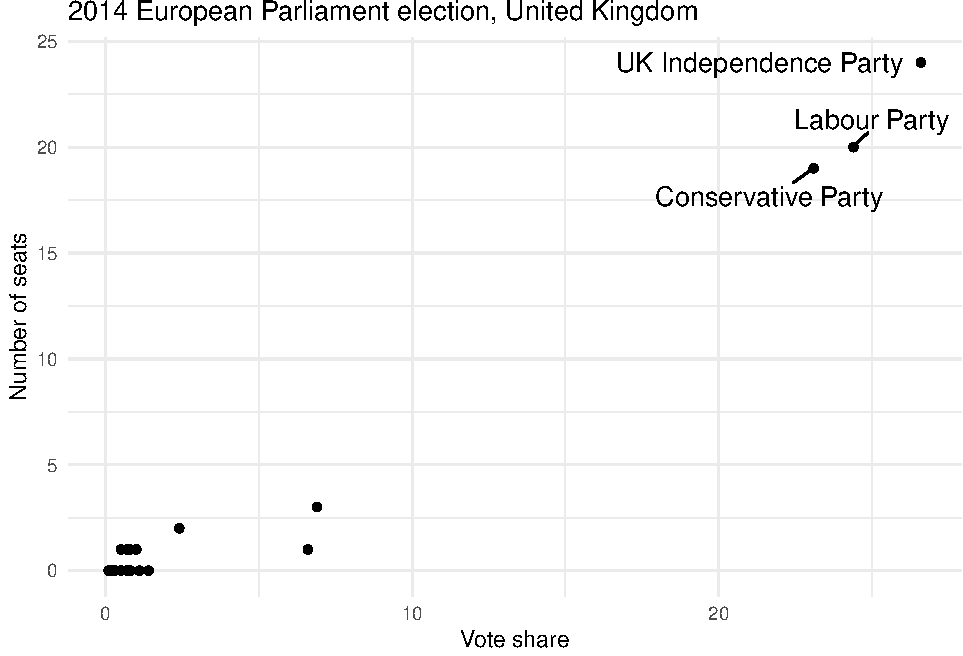
\includegraphics{qpolr_files/figure-latex/unnamed-chunk-128-1.pdf}
  
  \section{Scrape political speeches}\label{scrape-political-speeches}
  
  A lot of the text we can scrape online is not in the form of
  spreadsheets but in the form of nothing but text. To show how to scrape
  such text, we will focus on British political speeches from
  \url{http://www.britishpoliticalspeech.org/speech-archive.htm}.
  
  Specifically, we will select the speech the Leader's speech by Theresa
  May in Manchester from 2017. First, as in the previous example, we
  specify the url of the page we would like to scrape. In this speech,
  Theresa May is talking extensively about the British Dream.
  \begin{Shaded}
  \begin{Highlighting}[]
  \NormalTok{url <-}\StringTok{ }\KeywordTok{c}\NormalTok{(}
    \StringTok{"http://www.britishpoliticalspeech.org/speech-archive.htm?speech=367"}
  \NormalTok{  )}
  \end{Highlighting}
  \end{Shaded}
  To get the content of the page with the speech, we save the content of
  the page in the object \texttt{speechpage}.
  \begin{Shaded}
  \begin{Highlighting}[]
  \NormalTok{speechpage <-}\StringTok{ }\KeywordTok{read_html}\NormalTok{(url)}
  \end{Highlighting}
  \end{Shaded}
  Next, to select the actual part of the page containing the speech, we
  select the content within the
  \texttt{\textless{}p\textgreater{}\textless{}/p\textgreater{}} tags.
  \begin{Shaded}
  \begin{Highlighting}[]
  \NormalTok{data_speech <-}\StringTok{ }\KeywordTok{html_nodes}\NormalTok{(speechpage, }\StringTok{"p"}\NormalTok{)}
  \end{Highlighting}
  \end{Shaded}
  To get the actual text, we use the function \texttt{html\_text()}.
  \begin{Shaded}
  \begin{Highlighting}[]
  \NormalTok{data_speech_text <-}\StringTok{ }\KeywordTok{html_text}\NormalTok{(data_speech)}
  \end{Highlighting}
  \end{Shaded}
  Now we have all the text we need to use. However, to create a dataset
  with the words in the speech, we will use some functions from the
  package \texttt{tidytext} (as always, remember to install the package if
  you do not already have it installed) (Silge \& Robinson, 2016).
  \begin{Shaded}
  \begin{Highlighting}[]
  \KeywordTok{library}\NormalTok{(}\StringTok{"tidytext"}\NormalTok{)}
  \end{Highlighting}
  \end{Shaded}
  The first function we are going to use is not part of the package but
  will be used to convert our speech into a data frame using the
  \texttt{data\_frame()} function.
  \begin{Shaded}
  \begin{Highlighting}[]
  \NormalTok{data_speech_df <-}\StringTok{ }\KeywordTok{data_frame}\NormalTok{(}\DataTypeTok{text =}\NormalTok{ data_speech_text)}
  \end{Highlighting}
  \end{Shaded}
  While in a data frame, it is still just a lot of sentences on different
  rows. To unnest all the sentences in our text column into a word column,
  we use the function \texttt{unnest\_tokens()}.
  \begin{Shaded}
  \begin{Highlighting}[]
  \NormalTok{words <-}\StringTok{ }\NormalTok{data_speech_df }\OperatorTok\StringTok{ }\KeywordTok{unnest_tokens}\NormalTok{(word, text)}
  \end{Highlighting}
  \end{Shaded}
  This gives os an object, \texttt{words}, with 7,116 observations.
  However, a lot of these words are irrelevant stop words (most common
  words that we are not interested in such as \emph{the}, \emph{is},
  \emph{at}, \emph{which}) that we would like to remove. We use the
  \texttt{anti\_join()} function to remove all stop words.
  \begin{Shaded}
  \begin{Highlighting}[]
  \NormalTok{words <-}\StringTok{ }\NormalTok{words }\OperatorTok\StringTok{ }\KeywordTok{anti_join}\NormalTok{(stop_words, }\DataTypeTok{by =} \StringTok{"word"}\NormalTok{)}
  \end{Highlighting}
  \end{Shaded}
  Last, we can count the words in the speech and calculate the number of
  occurences.
  \begin{Shaded}
  \begin{Highlighting}[]
  \NormalTok{words }\OperatorTok\StringTok{ }\KeywordTok{count}\NormalTok{(word, }\DataTypeTok{sort =} \OtherTok{TRUE}\NormalTok{)}
  \end{Highlighting}
  \end{Shaded}
  \begin{verbatim}
  # A tibble: 1,280 x 2
     word        n
     <chr>   <int>
   1 people     49
   2 britain    36
   3 country    34
   4 dream      33
   5 world      30
   6 british    29
   7 that’s     21
   8 party      19
   9 it’s       17
  10 free       16
  # ... with 1,270 more rows
  \end{verbatim}
  We see that \emph{people} is mentioned 49 times, and \emph{britain} is
  mentioned 36 times. \emph{dream} and \emph{british} are mentioned 33 and
  29 times, respectively.
  
  \section{Get data from Twitter}\label{get-data-from-twitter}
  
  To get data from Twitter, we are going to use the \texttt{rtweet}
  package (Kearney, 2018). The first thing we do is to load the package
  (remember to install if if you have not already done so). You can find
  more information about the package here: \url{https://rtweet.info/}
  \begin{Shaded}
  \begin{Highlighting}[]
  \KeywordTok{library}\NormalTok{(}\StringTok{"rtweet"}\NormalTok{)}
  \end{Highlighting}
  \end{Shaded}
  Noteworthy, we cannot just collect data without any limits. In most
  cases, we have a liit of 18,000 observations per 15 minutes.
  
  \subsection{Data on twitter user}\label{data-on-twitter-user}
  
  To get data on a Twitter user, we can use different functions. There is
  a distinction betweeen friends and followers. The accounts a user
  follows are called friends, whereas followers are the accounts that
  follow a user. Here, we will use the \texttt{get\_friends()} function to
  get information on the people Donald Trump is following.
  \begin{Shaded}
  \begin{Highlighting}[]
  \NormalTok{trump_following <-}\StringTok{ }\KeywordTok{get_friends}\NormalTok{(}\StringTok{"realDonaldTrump"}\NormalTok{)}
  \end{Highlighting}
  \end{Shaded}
  When we do that, all we get is a series of user IDs for the people
  Donald Trump is following. We can use the \texttt{lookup\_users()}
  function toget more information about the individual accounts.
  \begin{Shaded}
  \begin{Highlighting}[]
  \NormalTok{trump_following <-}\StringTok{ }\KeywordTok{lookup_users}\NormalTok{(trump_following}\OperatorTok{$}\NormalTok{user_id)}
  \end{Highlighting}
  \end{Shaded}
  This gives us a lot more information on the individual users, including
  their Twitter handle, name and description. To see all the information
  saved, you can use the \texttt{names()} function.
  \begin{Shaded}
  \begin{Highlighting}[]
  \KeywordTok{names}\NormalTok{(trump_following)}
  \end{Highlighting}
  \end{Shaded}
  To save information on the user ID, the handle, name and the
  description, we create a new object called \texttt{trump\_data} just
  with these variables.
  \begin{Shaded}
  \begin{Highlighting}[]
  \NormalTok{trump_data <-}\StringTok{ }\NormalTok{trump_following }\OperatorTok\StringTok{ }
  \StringTok{  }\KeywordTok{select}\NormalTok{(user_id, screen_name, name, description) }
  \end{Highlighting}
  \end{Shaded}
  You can use \texttt{head(trump\_data)} to see what the data looks like.
  To get information on the followers of Donald Trump, you can use the
  \texttt{get\_followers()} function. However, this will take a lot of
  time to get (we are talking days!).
  
  To search for tweets from specific users, we can use the
  \texttt{search\_users()} function. Below, we search for tweets from
  users with \texttt{politics} (via Twitters search query).
  \begin{Shaded}
  \begin{Highlighting}[]
  \NormalTok{politics_users <-}\StringTok{ }\KeywordTok{search_users}\NormalTok{(}\StringTok{"politics"}\NormalTok{, }\DataTypeTok{n =} \DecValTok{50}\NormalTok{)}
  \end{Highlighting}
  \end{Shaded}
  Next, we can use the \texttt{get\_favorites()} function to get data on
  the tweets a user has favorited. Here, we save the favorites from Boris
  Johnson and save it in the object \texttt{tweets\_bj}.
  \begin{Shaded}
  \begin{Highlighting}[]
  \NormalTok{tweets_bj <-}\StringTok{ }\KeywordTok{get_favorites}\NormalTok{(}\StringTok{"BorisJohnson"}\NormalTok{)}
  \end{Highlighting}
  \end{Shaded}
  To get a sense of what this data looks like, you can use the
  \texttt{head()} function.
  \begin{Shaded}
  \begin{Highlighting}[]
  \KeywordTok{head}\NormalTok{(tweets_bj)}
  \end{Highlighting}
  \end{Shaded}
  \subsection{Data on trends}\label{data-on-trends}
  
  To get data on what is trending in a certain part of the world, we can
  use the \texttt{get\_trends()} function. Below, we get the 50 most
  trending topics in the United Kingdom. On October 29, 2018,
  \texttt{\#NationalCatDay} and \texttt{Angela\ Merkel} are both trending
  (not for the same reason though).
  \begin{Shaded}
  \begin{Highlighting}[]
  \NormalTok{trends_uk <-}\StringTok{ }\KeywordTok{get_trends}\NormalTok{(}\StringTok{"united kingdom"}\NormalTok{)}
  \end{Highlighting}
  \end{Shaded}
  \subsection{Data on tweets}\label{data-on-tweets}
  
  Last, to get data on specific tweets, we use the
  \texttt{search\_tweets()} function. Below, we get the most recent 100
  tweets mentioning \texttt{brexit}. We also specify that we are not
  interested in retweets.
  \begin{Shaded}
  \begin{Highlighting}[]
  \NormalTok{brexit <-}\StringTok{ }\KeywordTok{search_tweets}\NormalTok{(}
    \StringTok{"brexit"}\NormalTok{, }\DataTypeTok{n =} \DecValTok{100}\NormalTok{, }\DataTypeTok{include_rts =} \OtherTok{FALSE}
  \NormalTok{)}
  \end{Highlighting}
  \end{Shaded}
  This gives us a data frame with 100 observations and 88 variables. You
  can use the \texttt{names()} function to get a list of all variables in
  the data frame.
  
  \chapter*{(PART) Presenting data}\label{part-presenting-data}
  \addcontentsline{toc}{chapter}{(PART) Presenting data}
  
  \chapter{Data visualisation}\label{dataviz}
  
  Visualising data is important (Healy \& Moody, 2014). As with everything
  in \texttt{R}, there are a lot of different ways to visualise data. One
  simple way to visualise data is to use \emph{base} functions in
  \texttt{R} (i.e.~functions that come when you install the \texttt{R}
  language). Below you will see an example on this.
  \begin{Shaded}
  \begin{Highlighting}[]
  \KeywordTok{plot}\NormalTok{(}\DataTypeTok{x=}\NormalTok{uk2017}\OperatorTok{$}\NormalTok{votes, }\DataTypeTok{y=}\NormalTok{uk2017}\OperatorTok{$}\NormalTok{seats)}
  \end{Highlighting}
  \end{Shaded}
  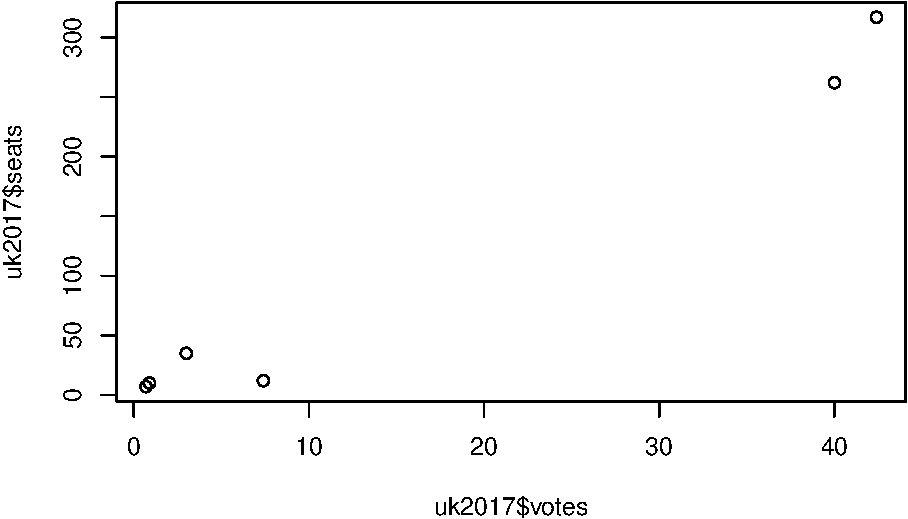
\includegraphics{qpolr_files/figure-latex/unnamed-chunk-148-1.pdf}
  
  There is nothing inherently wrong with using a function like this, but
  the moment we want to tweak the figure, it gets complicated.
  Accordingly, we will not use the standard functions in \texttt{R} but
  the package \texttt{ggplot2} (H. Wickham, 2009). This package makes it
  easy to create beautiful figures in \texttt{R}.
  
  \texttt{ggplot2} creates more beautiful figures with better defaults, it
  is very customizable, and it works within the tidyverse (together with
  \texttt{dplyr}). For those reasons it is becoming incredibly popular
  among practitioners and academics alike. That being said, there is an
  element of personal preference when it comes to data visualisations and
  \texttt{ggplot2} is not perfect. While the defaults are good, they could
  be better. Furthermore, there are functions in the package you should
  \emph{never} use (such as \texttt{qplot()}, short for \emph{quick
  plot}).
  
  \section{\texorpdfstring{The basics of
  \texttt{ggplot2}}{The basics of ggplot2}}\label{the-basics-of-ggplot2}
  
  You can load \texttt{ggplot2} by loading the \texttt{tidyverse}
  (alternatively you can just load the \texttt{ggplot2} package).
  \begin{Shaded}
  \begin{Highlighting}[]
  \KeywordTok{library}\NormalTok{(}\StringTok{"tidyverse"}\NormalTok{)}
  \end{Highlighting}
  \end{Shaded}
  The two g's (\texttt{gg}) in \texttt{ggplot2} are short for
  \emph{grammar of graphics}. The philosophy is that we are working with
  building blocks in the form of a sentence structure where we can add
  more components to our visualisation, e.g.~change colours and add text.
  This makes it easy to first create a figure and then tweak it till we
  are satisfied.
  
  These building blocks are:
  \begin{enumerate}
  \def\labelenumi{\arabic{enumi}.}
  \tightlist
  \item
    Data (the data frame we will be using)
  \item
    Aesthetics (the variables we will be working with)
  \item
    Geometric objects (the type of visualisation)
  \item
    Theme adjustments (size, text, colours etc.)
  \end{enumerate}
  \subsection{Data}\label{data}
  
  The function we will be using is \texttt{ggplot()}. Here, we will be
  using the \texttt{states} data from the \texttt{poliscidata} package
  introduced in Chapter \ref{datadownload}.
  \begin{Shaded}
  \begin{Highlighting}[]
  \KeywordTok{library}\NormalTok{(}\StringTok{"poliscidata"}\NormalTok{)}
  \NormalTok{states <-}\StringTok{ }\NormalTok{states}
  \end{Highlighting}
  \end{Shaded}
  The first thing we always have to specify in our function is the data
  frame. In other words, you will \emph{always} have to use a data frame.
  \begin{Shaded}
  \begin{Highlighting}[]
  \KeywordTok{ggplot}\NormalTok{(states)}
  \end{Highlighting}
  \end{Shaded}
  Do note that if you run the code above - and have the \texttt{states} in
  your working memory, we will not get anything but an empty plot. The
  only thing we have done so far is telling \texttt{R} that we would like
  to create a coordinate system and data from \texttt{uk2017} should play
  some role, but this is of course not enough.
  
  \subsection{Aesthetics}\label{aesthetics}
  
  The next thing we have to specify is what variables in the data frame we
  will be using and what role they play. To do this we will use the
  function \texttt{aes()} \emph{within} the \texttt{ggplot()} function
  after the data frame (remember the comma after the data frame).
  \begin{Shaded}
  \begin{Highlighting}[]
  \KeywordTok{ggplot}\NormalTok{(states, }\KeywordTok{aes}\NormalTok{(}\DataTypeTok{x =}\NormalTok{ abort_rate08, }\DataTypeTok{y =}\NormalTok{ obama2012))}
  \end{Highlighting}
  \end{Shaded}
  In the example above we specify that we are working with \emph{two}
  variables, x (Number of abortions per 1,000 women aged 15-44 in 2008)
  and y (Obama vote share in 2012). If you only will be working with one
  variable (e.g.~a histogram), you should of course only specificy one
  variable, x. However, now we have only told \texttt{R} what variables we
  would like to work with, but it is still not enough to actually create a
  figure.
  
  \subsection{Geometric objects}\label{geometric-objects}
  
  Now we will need to add the geometric object, we would like to
  visualise. We need to go to a new line and tell \texttt{R} to follow
  along. To do this, we add a plus (\texttt{+}) at the end of the line. On
  the new line we add the type of geometric object (\texttt{geom\_}), we
  want add. To replicate the plot above we use \texttt{geom\_point()}.
  \begin{Shaded}
  \begin{Highlighting}[]
  \KeywordTok{ggplot}\NormalTok{(states, }\KeywordTok{aes}\NormalTok{(}\DataTypeTok{x =}\NormalTok{ abort_rate08, }\DataTypeTok{y =}\NormalTok{ obama2012)) }\OperatorTok{+}
  \StringTok{  }\KeywordTok{geom_point}\NormalTok{()}
  \end{Highlighting}
  \end{Shaded}
  \begin{center}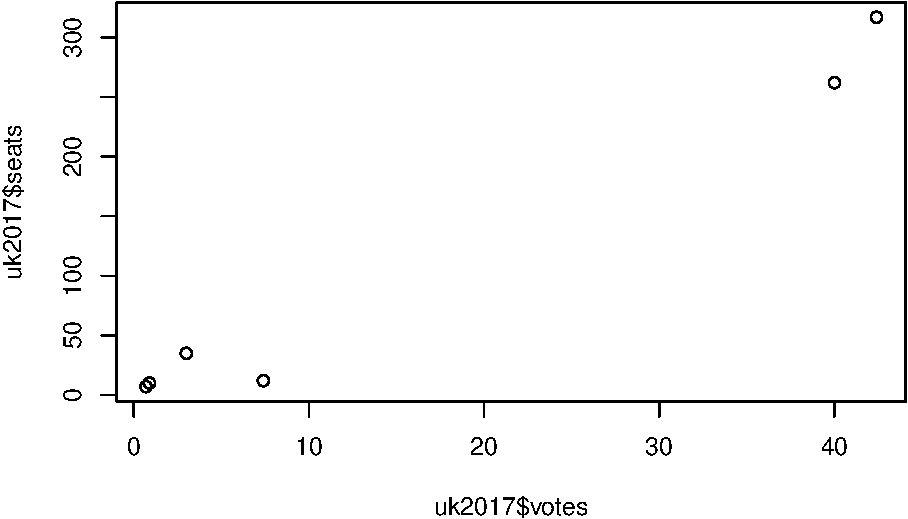
\includegraphics{qpolr_files/figure-latex/unnamed-chunk-153-1} \end{center}
  
  This is a standard \texttt{ggplot2} plot with all its defaults. If we
  instead a scatter plot wanted a line plot, we can change
  \texttt{geom\_point()} to \texttt{geom\_line()}.
  \begin{Shaded}
  \begin{Highlighting}[]
  \KeywordTok{ggplot}\NormalTok{(states, }\KeywordTok{aes}\NormalTok{(}\DataTypeTok{x =}\NormalTok{ abort_rate08, }\DataTypeTok{y =}\NormalTok{ obama2012)) }\OperatorTok{+}
  \StringTok{  }\KeywordTok{geom_line}\NormalTok{()}
  \end{Highlighting}
  \end{Shaded}
  \begin{center}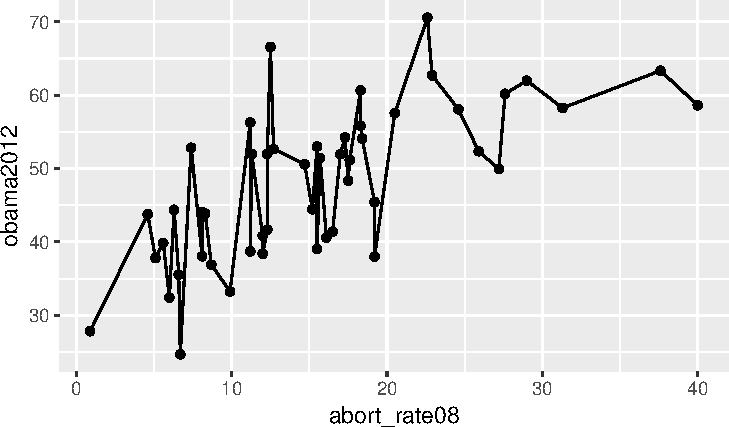
\includegraphics{qpolr_files/figure-latex/unnamed-chunk-154-1} \end{center}
  
  The above figure is somewhat misleading so it is just to show the logic
  of the how geometric objects work. Interestingly, we can add multiple
  geometric objects to the same plot. Below, we add both geometric objects
  used above.
  \begin{Shaded}
  \begin{Highlighting}[]
  \KeywordTok{ggplot}\NormalTok{(states, }\KeywordTok{aes}\NormalTok{(}\DataTypeTok{x =}\NormalTok{ abort_rate08, }\DataTypeTok{y =}\NormalTok{ obama2012)) }\OperatorTok{+}
  \StringTok{  }\KeywordTok{geom_line}\NormalTok{() }\OperatorTok{+}
  \StringTok{  }\KeywordTok{geom_point}\NormalTok{()}
  \end{Highlighting}
  \end{Shaded}
  \begin{center}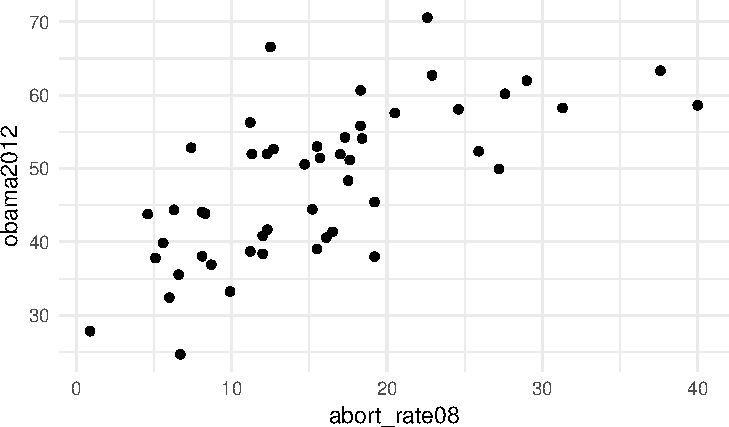
\includegraphics{qpolr_files/figure-latex/unnamed-chunk-155-1} \end{center}
  
  \subsection{Theme adjustments}\label{theme-adjustments}
  
  What you will see in a typical plot is that it is not done. The axes
  simply have the variable names, the colours are not great etc.
  Accordingly, we often need to add and change elements of our plot. Here
  we add the theme of the plot (described in detail below).
  \begin{Shaded}
  \begin{Highlighting}[]
  \KeywordTok{ggplot}\NormalTok{(states, }\KeywordTok{aes}\NormalTok{(}\DataTypeTok{x =}\NormalTok{ abort_rate08, }\DataTypeTok{y =}\NormalTok{ obama2012)) }\OperatorTok{+}
  \StringTok{  }\KeywordTok{geom_point}\NormalTok{() }\OperatorTok{+}
  \StringTok{  }\KeywordTok{theme_minimal}\NormalTok{()}
  \end{Highlighting}
  \end{Shaded}
  \begin{center}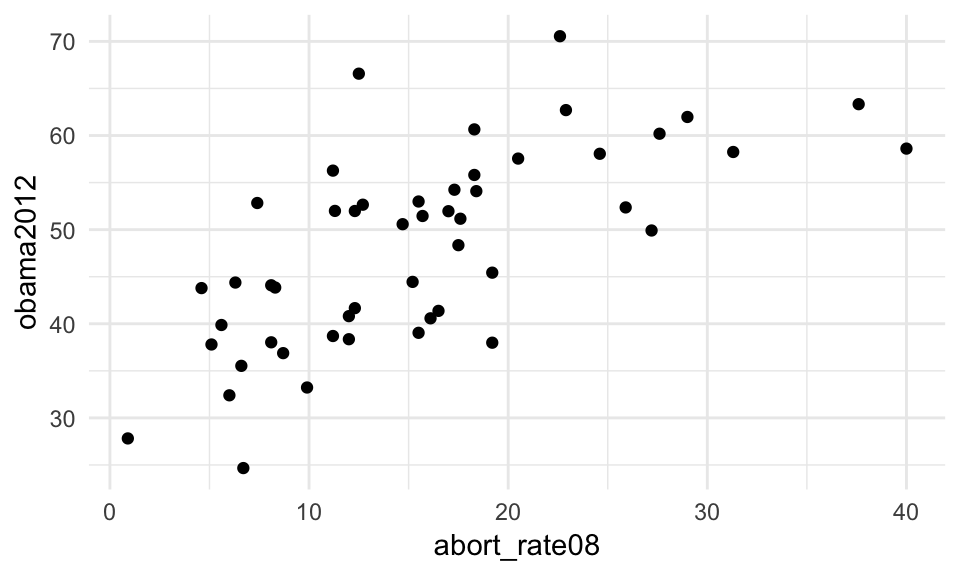
\includegraphics{qpolr_files/figure-latex/unnamed-chunk-156-1} \end{center}
  
  We can also easily change the labels by using \texttt{xlab()} and
  \texttt{ylab()}.
  \begin{Shaded}
  \begin{Highlighting}[]
  \KeywordTok{ggplot}\NormalTok{(states, }\KeywordTok{aes}\NormalTok{(}\DataTypeTok{x =}\NormalTok{ abort_rate08, }\DataTypeTok{y =}\NormalTok{ obama2012)) }\OperatorTok{+}
  \StringTok{  }\KeywordTok{geom_point}\NormalTok{() }\OperatorTok{+}
  \StringTok{  }\KeywordTok{theme_minimal}\NormalTok{() }\OperatorTok{+}
  \StringTok{  }\KeywordTok{ylab}\NormalTok{(}\StringTok{"Obama vote share in 2012"}\NormalTok{) }\OperatorTok{+}
  \StringTok{  }\KeywordTok{xlab}\NormalTok{(}\StringTok{"Number of abortions per 1,000 women aged 15-44 in 2008"}\NormalTok{)}
  \end{Highlighting}
  \end{Shaded}
  \begin{center}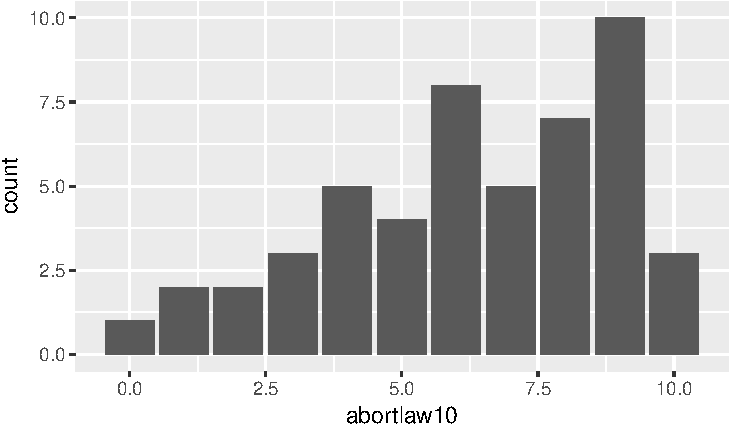
\includegraphics{qpolr_files/figure-latex/unnamed-chunk-157-1} \end{center}
  
  This is the basic logic of \texttt{ggplot2}.
  
  \section{Plotting one variable:
  distributions}\label{plotting-one-variable-distributions}
  
  Table \ref{tab:distributions} shows the geometric objects we will be
  working with below. In addition to the name of the object, you will also
  find a link where you can find more illustrations and examples on how
  they work.
  \begin{longtable}[]{@{}lll@{}}
  \caption{\label{tab:distributions} Selected geometric objects with
  \texttt{ggplot2}}\tabularnewline
  \toprule
  Name & Function & Cookbook for R\tabularnewline
  \midrule
  \endfirsthead
  \toprule
  Name & Function & Cookbook for R\tabularnewline
  \midrule
  \endhead
  Bar plot & \texttt{geom\_bar()} &
  \href{http://www.cookbook-r.com/Graphs/Bar_and_line_graphs_(ggplot2)/}{Bar
  and line graphs}\tabularnewline
  Histogram & \texttt{geom\_histogram()} &
  \href{http://www.cookbook-r.com/Graphs/Plotting_distributions_(ggplot2)/}{Plotting
  distributions}\tabularnewline
  Density plot & \texttt{geom\_density()} &
  \href{http://www.cookbook-r.com/Graphs/Plotting_distributions_(ggplot2)/}{Plotting
  distributions}\tabularnewline
  \bottomrule
  \end{longtable}
  \subsection{Bar plot}\label{bar-plot}
  
  The first plot we will do is a bar plot. To do this we use a variable on
  the number of restrictions on abortion (\texttt{abortlaw10}) and
  \texttt{geom\_bar()}.
  \begin{Shaded}
  \begin{Highlighting}[]
  \KeywordTok{ggplot}\NormalTok{(states, }\KeywordTok{aes}\NormalTok{(}\DataTypeTok{x=}\NormalTok{abortlaw10)) }\OperatorTok{+}
  \StringTok{  }\KeywordTok{geom_bar}\NormalTok{() }
  \end{Highlighting}
  \end{Shaded}
  \begin{center}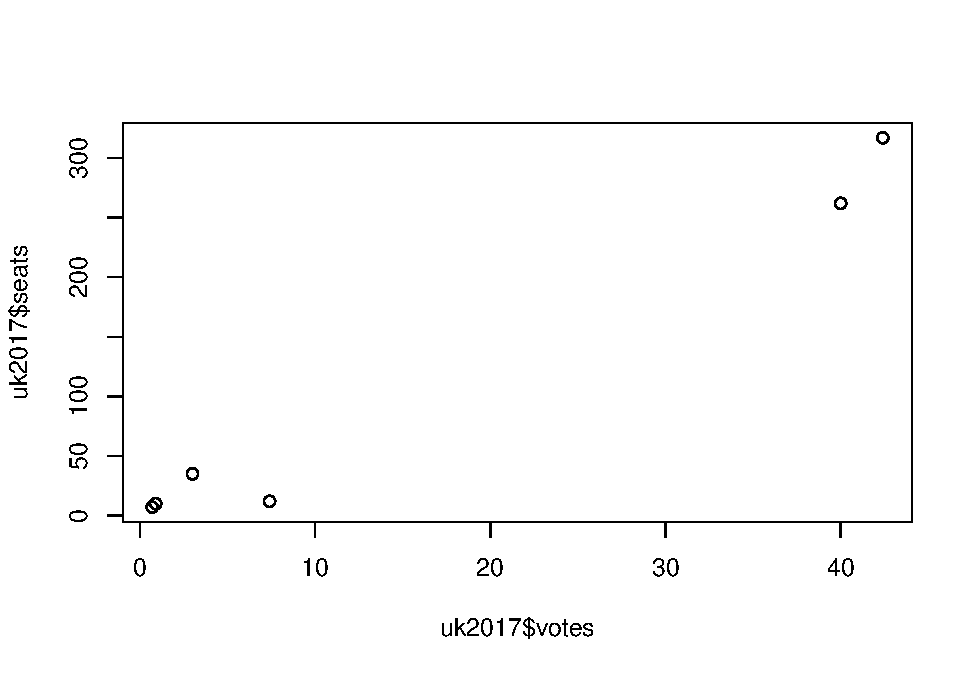
\includegraphics{qpolr_files/figure-latex/unnamed-chunk-158-1} \end{center}
  
  \subsection{Histograms}\label{histograms}
  
  The next figure we will work with is the histogram. Here we will plot
  the distribution of Obama's vote share in 2012 (the \texttt{obama2012}
  variable) and use \texttt{geom\_histogram()}.
  \begin{Shaded}
  \begin{Highlighting}[]
  \KeywordTok{ggplot}\NormalTok{(states, }\KeywordTok{aes}\NormalTok{(}\DataTypeTok{x=}\NormalTok{obama2012)) }\OperatorTok{+}
  \StringTok{  }\KeywordTok{geom_histogram}\NormalTok{() }
  \end{Highlighting}
  \end{Shaded}
  \begin{verbatim}
  `stat_bin()` using `bins = 30`. Pick better value with `binwidth`.
  \end{verbatim}
  \begin{center}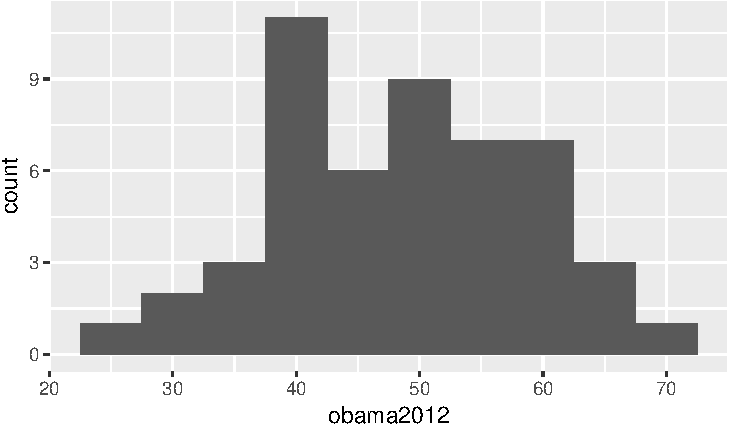
\includegraphics{qpolr_files/figure-latex/unnamed-chunk-159-1} \end{center}
  
  As you can see, we get a message about the use of a default binwidth.
  This is to emphasize the importance of specifying the binwidth yourself.
  We can change the bin width by adding \texttt{binwidth} to
  \texttt{geom\_histogram()}.
  \begin{Shaded}
  \begin{Highlighting}[]
  \KeywordTok{ggplot}\NormalTok{(states, }\KeywordTok{aes}\NormalTok{(}\DataTypeTok{x=}\NormalTok{obama2012)) }\OperatorTok{+}
  \StringTok{  }\KeywordTok{geom_histogram}\NormalTok{(}\DataTypeTok{binwidth =} \DecValTok{5}\NormalTok{)}
  \end{Highlighting}
  \end{Shaded}
  \begin{center}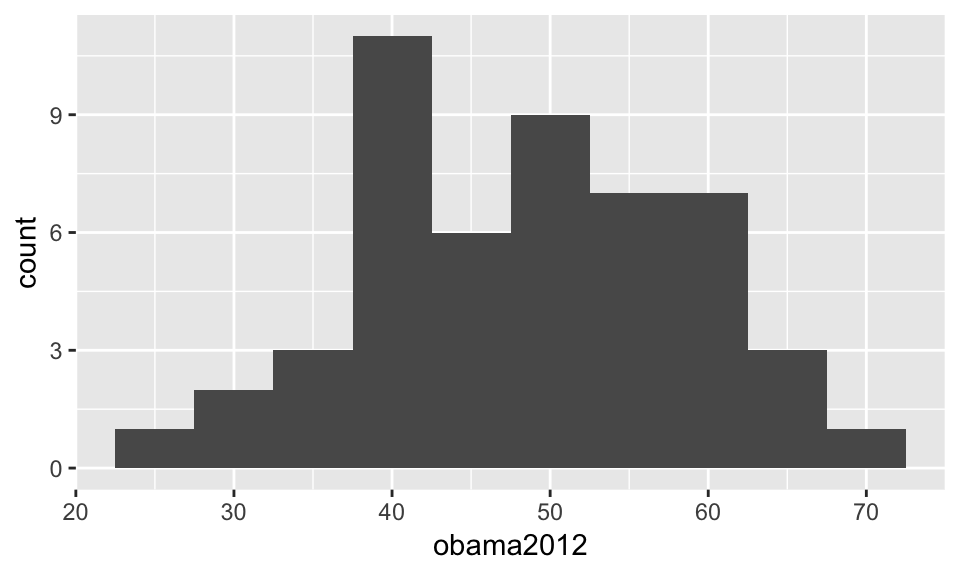
\includegraphics{qpolr_files/figure-latex/unnamed-chunk-160-1} \end{center}
  
  Play around with different binwidths to see how it affects the
  distribution in the figure.
  
  \subsection{Density plots}\label{density-plots}
  
  The histogram is not the only way to show the distribution of a
  variable. To make a density plot, you can use \texttt{geom\_density()}.
  We use the \texttt{obama2012} variable again.
  \begin{Shaded}
  \begin{Highlighting}[]
  \KeywordTok{ggplot}\NormalTok{(states, }\KeywordTok{aes}\NormalTok{(}\DataTypeTok{x=}\NormalTok{obama2012)) }\OperatorTok{+}
  \StringTok{  }\KeywordTok{geom_density}\NormalTok{() }
  \end{Highlighting}
  \end{Shaded}
  \begin{center}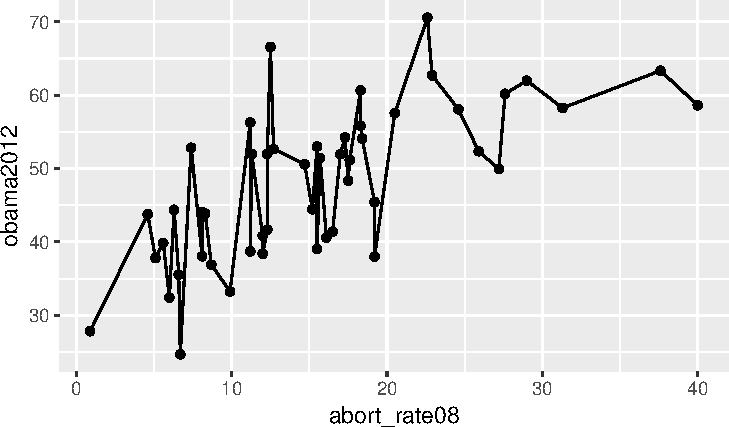
\includegraphics{qpolr_files/figure-latex/unnamed-chunk-161-1} \end{center}
  
  Do compare the density plot to the histograms above.
  
  \section{Plotting two variables:
  relationships}\label{plotting-two-variables-relationships}
  
  To show how different variables are related, Table
  \ref{tab:distributions} shows the geometric objects we will be working
  with below as well as link where you can find more information.
  \begin{longtable}[]{@{}lll@{}}
  \caption{\label{tab:relationships} Selected geometric objects for relations
  in \texttt{ggplot2}}\tabularnewline
  \toprule
  Name & Function & Cookbook for R\tabularnewline
  \midrule
  \endfirsthead
  \toprule
  Name & Function & Cookbook for R\tabularnewline
  \midrule
  \endhead
  Box plot & \texttt{geom\_boxplot()} &
  \href{http://www.cookbook-r.com/Graphs/Plotting_distributions_(ggplot2)/}{Plotting
  distributions}\tabularnewline
  Scatter plot & \texttt{geom\_point()} &
  \href{http://www.cookbook-r.com/Graphs/Scatterplots_(ggplot2)/}{Scatterplots}\tabularnewline
  \bottomrule
  \end{longtable}
  \subsection{Box plot}\label{box-plot}
  
  For the box plot, we will be using \texttt{geom\_boxplot()} to show how
  the vote share for Obama is related to abortion laws (here with the
  \texttt{abortlaw3} variable, i.e.~abortion restrictions with three tiers
  of number of restrictions).
  \begin{Shaded}
  \begin{Highlighting}[]
  \KeywordTok{ggplot}\NormalTok{(states, }\KeywordTok{aes}\NormalTok{(}\DataTypeTok{x=}\NormalTok{abortlaw3, }\DataTypeTok{group=}\NormalTok{abortlaw3, }\DataTypeTok{y=}\NormalTok{obama2012)) }\OperatorTok{+}
  \StringTok{  }\KeywordTok{geom_boxplot}\NormalTok{() }
  \end{Highlighting}
  \end{Shaded}
  \begin{center}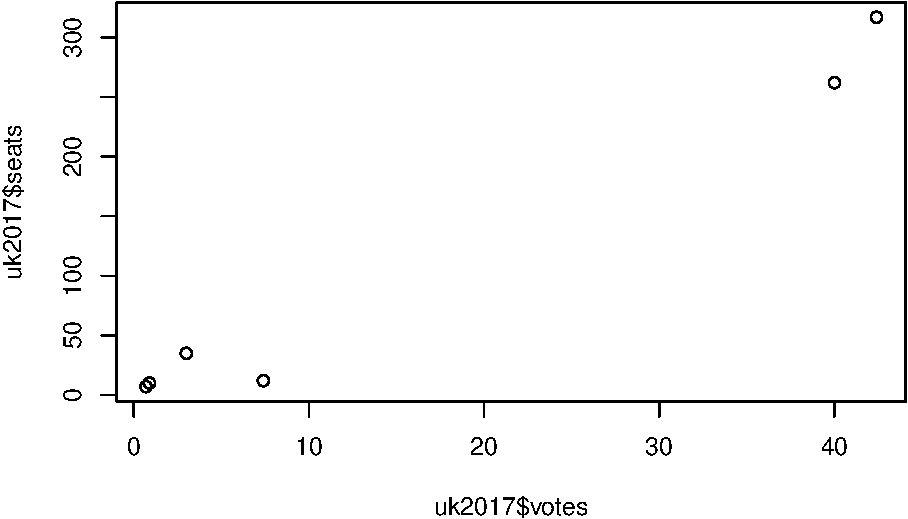
\includegraphics{qpolr_files/figure-latex/unnamed-chunk-162-1} \end{center}
  
  Here we can see that Obama got a greater vote share in states with less
  restrictions on abortion.
  
  \subsection{Scatter plots}\label{scatter-plots}
  
  To illustrate the relation between number of abortions and Obama's vote
  share, measured with the variables \texttt{abort\_rate08} and
  \texttt{obama2012}, we will create a scatter plot with
  \texttt{geom\_point()}.
  \begin{Shaded}
  \begin{Highlighting}[]
  \KeywordTok{ggplot}\NormalTok{(states, }\KeywordTok{aes}\NormalTok{(}\DataTypeTok{x=}\NormalTok{abort_rate08, }\DataTypeTok{y=}\NormalTok{obama2012)) }\OperatorTok{+}
  \StringTok{  }\KeywordTok{geom_point}\NormalTok{() }
  \end{Highlighting}
  \end{Shaded}
  \begin{center}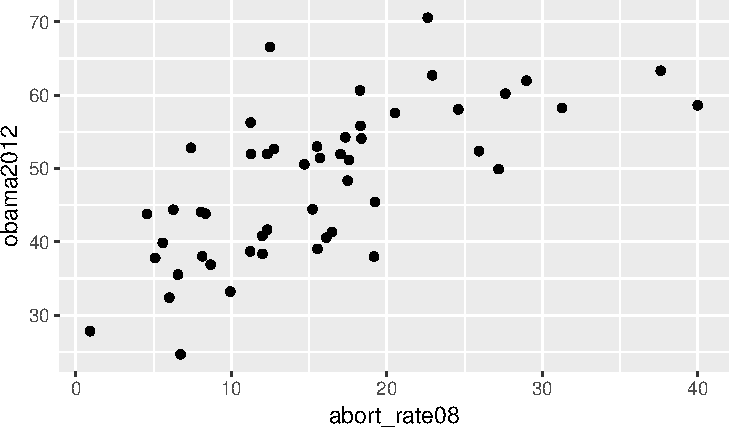
\includegraphics{qpolr_files/figure-latex/unnamed-chunk-163-1} \end{center}
  
  If we are working with a lot of observations, there will be an overlap
  in the points. To show all of the observations, we can add some small,
  random noise to the observations, so we can see more of them. To do
  this, we can use \texttt{geom\_jitter()} instead of
  \texttt{geom\_point()}.
  \begin{Shaded}
  \begin{Highlighting}[]
  \KeywordTok{ggplot}\NormalTok{(states, }\KeywordTok{aes}\NormalTok{(}\DataTypeTok{x=}\NormalTok{abort_rate08, }\DataTypeTok{y=}\NormalTok{obama2012)) }\OperatorTok{+}
  \StringTok{  }\KeywordTok{geom_jitter}\NormalTok{() }
  \end{Highlighting}
  \end{Shaded}
  \begin{center}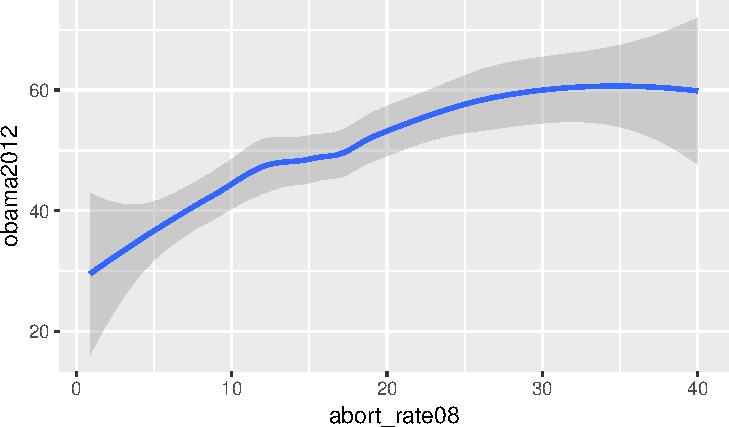
\includegraphics{qpolr_files/figure-latex/unnamed-chunk-164-1} \end{center}
  
  We can also use \texttt{geom\_point(position\ =\ "jitter")} instead of
  Instead of \texttt{geom\_jitter()}. However, in this particular case, as
  we only have 50 observations, it is not a major concern.
  
  \subsection{Line plots}\label{line-plots}
  
  To create a regression line we can use the \texttt{geom\_smooth()}
  function. Here we will again look at the relation between
  \texttt{abort\_rate08} and \texttt{obama2012}.
  \begin{Shaded}
  \begin{Highlighting}[]
  \KeywordTok{ggplot}\NormalTok{(states, }\KeywordTok{aes}\NormalTok{(}\DataTypeTok{x=}\NormalTok{abort_rate08, }\DataTypeTok{y=}\NormalTok{obama2012)) }\OperatorTok{+}
  \StringTok{  }\KeywordTok{geom_smooth}\NormalTok{()}
  \end{Highlighting}
  \end{Shaded}
  \begin{center}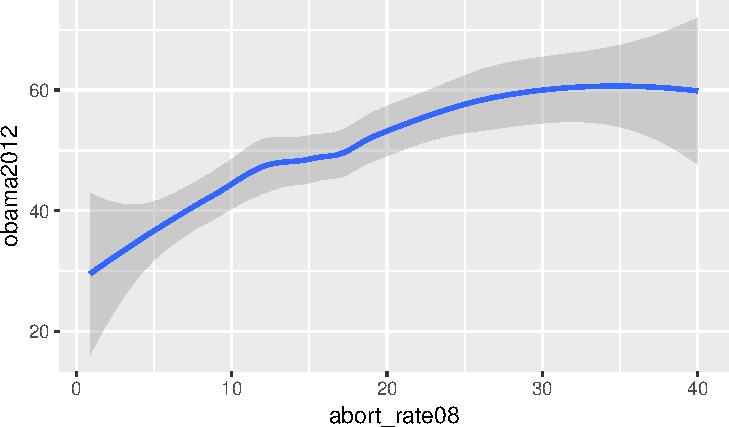
\includegraphics{qpolr_files/figure-latex/unnamed-chunk-165-1} \end{center}
  
  Here we can see that as the abortion rate increases, so does the vote
  share for Obama. As we can also see, this is a smoothing function. To
  have a linear line instead we can specify that we will be using
  \texttt{method="lm"} as an option.
  \begin{Shaded}
  \begin{Highlighting}[]
  \KeywordTok{ggplot}\NormalTok{(states, }\KeywordTok{aes}\NormalTok{(}\DataTypeTok{x=}\NormalTok{abort_rate08, }\DataTypeTok{y=}\NormalTok{obama2012)) }\OperatorTok{+}
  \StringTok{  }\KeywordTok{geom_smooth}\NormalTok{(}\DataTypeTok{method=}\StringTok{"lm"}\NormalTok{)}
  \end{Highlighting}
  \end{Shaded}
  \begin{center}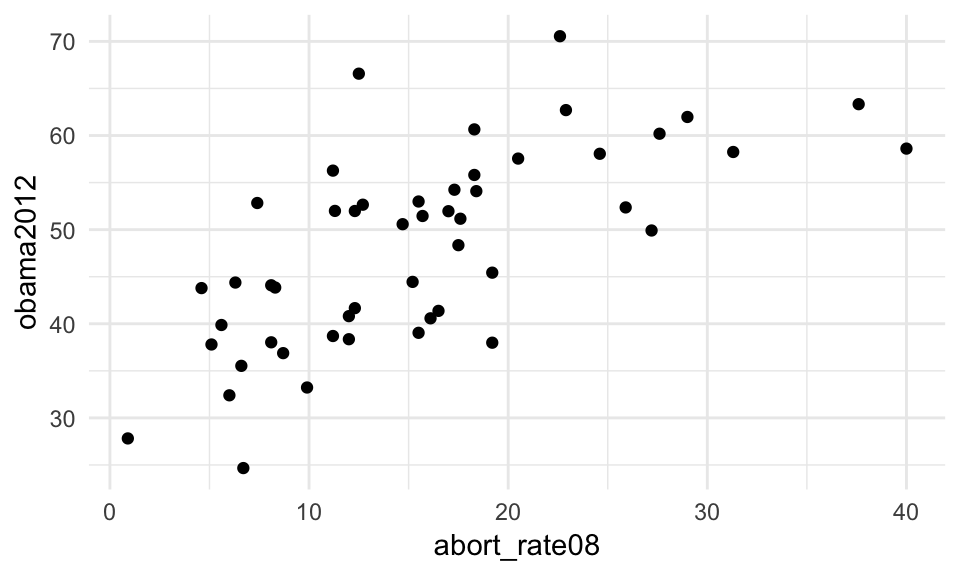
\includegraphics{qpolr_files/figure-latex/unnamed-chunk-166-1} \end{center}
  
  \section{Manipulating plots}\label{manipulating-plots}
  
  \subsection{Themes}\label{themes}
  
  As you could see in the plots above, we have used a default theme in
  \texttt{ggplot2}. Table \ref{tab:ggthemes} shows a series of themes to
  be found in \texttt{ggplot2}and the package
  \href{https://cran.r-project.org/web/packages/ggthemes/vignettes/ggthemes.html}{\texttt{ggthemes}}.
  These are just a selection of some of the themes.
  \begin{longtable}[]{@{}lll@{}}
  \caption{\label{tab:ggthemes} Selected themes for
  \texttt{ggplot2}}\tabularnewline
  \toprule
  Function & Package & Description\tabularnewline
  \midrule
  \endfirsthead
  \toprule
  Function & Package & Description\tabularnewline
  \midrule
  \endhead
  theme\_bw() & \texttt{ggplot2} & Black elements on white
  background\tabularnewline
  theme\_minimal() & \texttt{ggplot2} & Minimalistic\tabularnewline
  theme\_classic() & \texttt{ggplot2} & Theme without grid
  lines\tabularnewline
  theme\_base() & \texttt{ggthemes} & Copy of the base theme in
  \texttt{R}\tabularnewline
  theme\_economist() & \texttt{ggthemes} & The Economist
  theme\tabularnewline
  theme\_fivethirtyeight() & \texttt{ggthemes} & FiveThirtyEight
  theme\tabularnewline
  theme\_tufte() & \texttt{ggthemes} & Tufte (1983) theme\tabularnewline
  \bottomrule
  \end{longtable}
  Figure \ref{fig:ggthemes} shows the look of the different themes. The
  order is: Standard, \texttt{theme\_bw()}, \texttt{theme\_minimal()},
  \texttt{theme\_classic()}, \texttt{theme\_base()},
  \texttt{theme\_economist()}, \texttt{theme\_fivethirtyeight()},
  \texttt{theme\_tufte()}.
  \begin{figure}
  \centering
  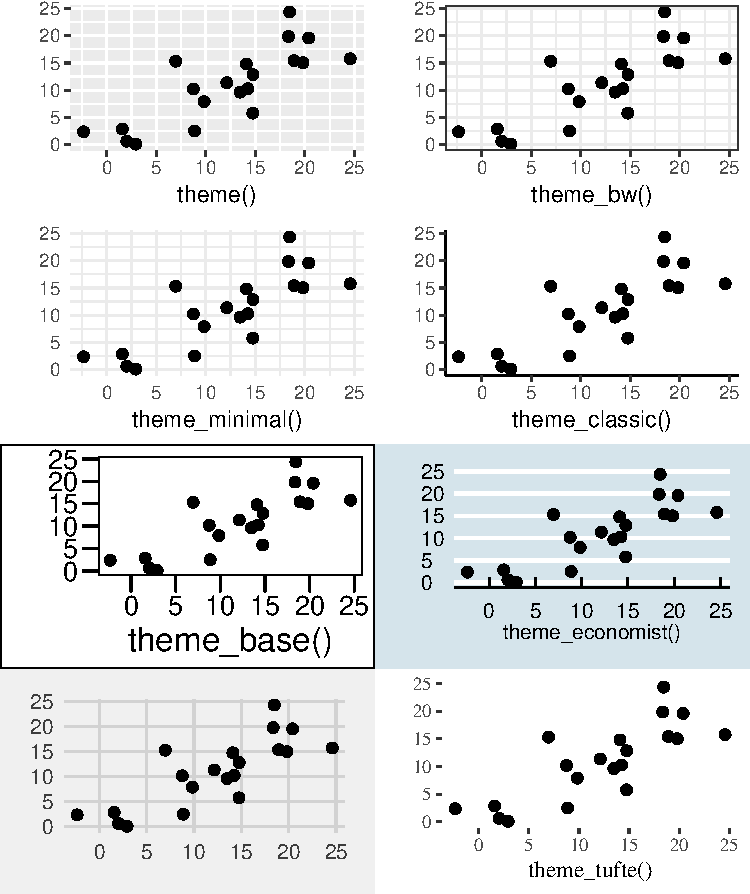
\includegraphics{qpolr_files/figure-latex/ggthemes-1.pdf}
  \caption{\label{fig:ggthemes}Eight themes}
  \end{figure}
  You can find a lot more resources online related to \texttt{ggplot2}. In
  addition to the links above, do consult
  \href{https://github.com/cttobin/ggthemr}{ggthemr} and
  \href{https://www.ggplot2-exts.org/}{ggplot2 extensions}.
  
  Below, we will be using \texttt{theme\_minimal()} as the theme when we
  work with out plots.
  \begin{Shaded}
  \begin{Highlighting}[]
  \KeywordTok{ggplot}\NormalTok{(states, }\KeywordTok{aes}\NormalTok{(}\DataTypeTok{x=}\NormalTok{abort_rate08, }\DataTypeTok{y=}\NormalTok{obama2012)) }\OperatorTok{+}
  \StringTok{  }\KeywordTok{geom_point}\NormalTok{(}\DataTypeTok{position =} \StringTok{"jitter"}\NormalTok{) }\OperatorTok{+}\StringTok{ }
  \StringTok{  }\KeywordTok{geom_smooth}\NormalTok{(}\DataTypeTok{se=}\OtherTok{FALSE}\NormalTok{) }\OperatorTok{+}
  \StringTok{  }\KeywordTok{theme_minimal}\NormalTok{()}
  \end{Highlighting}
  \end{Shaded}
  \begin{center}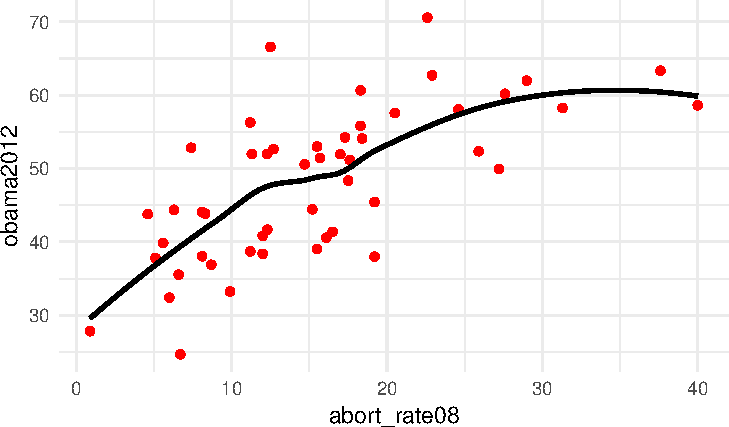
\includegraphics{qpolr_files/figure-latex/unnamed-chunk-167-1} \end{center}
  
  \subsection{Colours}\label{colours}
  
  If we want to change the colours of the points in our plot, we can add
  the \texttt{colour=""} option to our geometric objects. In the example
  below we change the colour of our points from black to red and the
  colour of the line to black.
  \begin{Shaded}
  \begin{Highlighting}[]
  \KeywordTok{ggplot}\NormalTok{(states, }\KeywordTok{aes}\NormalTok{(}\DataTypeTok{x=}\NormalTok{abort_rate08, }\DataTypeTok{y=}\NormalTok{obama2012)) }\OperatorTok{+}
  \StringTok{  }\KeywordTok{geom_point}\NormalTok{(}\DataTypeTok{colour=}\StringTok{"red"}\NormalTok{) }\OperatorTok{+}\StringTok{ }
  \StringTok{  }\KeywordTok{geom_smooth}\NormalTok{(}\DataTypeTok{se=}\OtherTok{FALSE}\NormalTok{, }\DataTypeTok{colour=}\StringTok{"black"}\NormalTok{) }\OperatorTok{+}
  \StringTok{  }\KeywordTok{theme_minimal}\NormalTok{()}
  \end{Highlighting}
  \end{Shaded}
  \begin{center}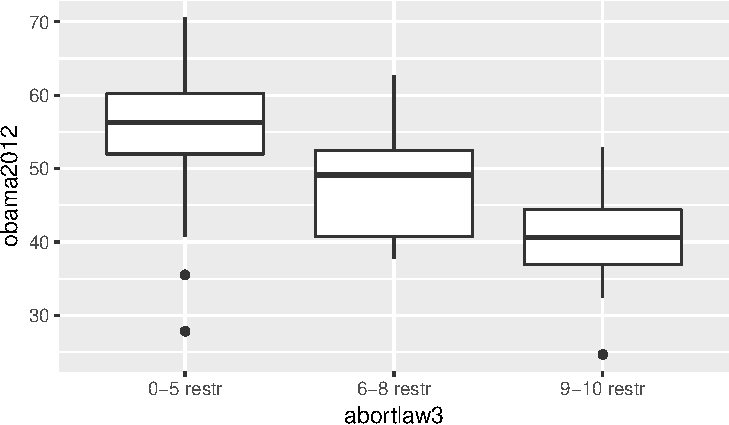
\includegraphics{qpolr_files/figure-latex/unnamed-chunk-168-1} \end{center}
  
  If we want to give points a value based on the value of a specific
  variable, we need to specificy this within \texttt{aes()}. When we add
  \texttt{colour=abortlaw3} to our \texttt{aes()}, we will see different
  colours for states with different restrictions on abortion.
  \begin{Shaded}
  \begin{Highlighting}[]
  \KeywordTok{ggplot}\NormalTok{(states, }\KeywordTok{aes}\NormalTok{(}\DataTypeTok{x=}\NormalTok{abort_rate08, }\DataTypeTok{y=}\NormalTok{obama2012)) }\OperatorTok{+}
  \StringTok{  }\KeywordTok{geom_point}\NormalTok{(}\KeywordTok{aes}\NormalTok{(}\DataTypeTok{colour=}\NormalTok{abortlaw3)) }\OperatorTok{+}\StringTok{ }
  \StringTok{  }\KeywordTok{geom_smooth}\NormalTok{(}\DataTypeTok{se=}\OtherTok{FALSE}\NormalTok{, }\DataTypeTok{colour=}\StringTok{"black"}\NormalTok{) }\OperatorTok{+}
  \StringTok{  }\KeywordTok{theme_minimal}\NormalTok{()}
  \end{Highlighting}
  \end{Shaded}
  \begin{center}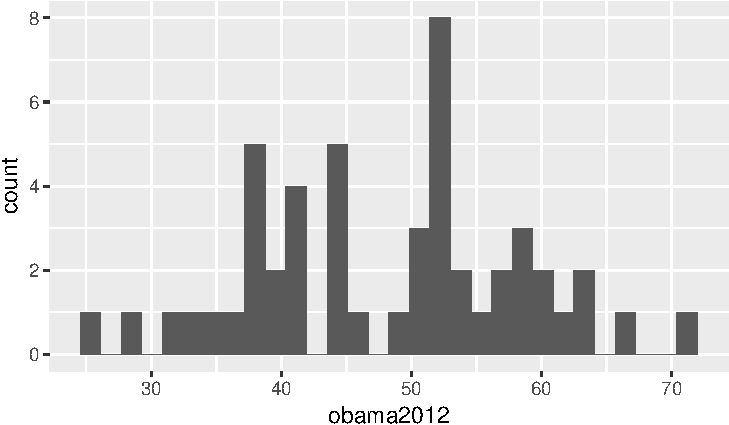
\includegraphics{qpolr_files/figure-latex/unnamed-chunk-169-1} \end{center}
  
  If we want to change these colours, we can use
  \texttt{scale\_colour\_manual()}.
  \begin{Shaded}
  \begin{Highlighting}[]
  \KeywordTok{ggplot}\NormalTok{(states, }\KeywordTok{aes}\NormalTok{(}\DataTypeTok{x=}\NormalTok{abort_rate08, }\DataTypeTok{y=}\NormalTok{obama2012)) }\OperatorTok{+}
  \StringTok{  }\KeywordTok{geom_point}\NormalTok{(}\KeywordTok{aes}\NormalTok{(}\DataTypeTok{colour=}\NormalTok{abortlaw3)) }\OperatorTok{+}\StringTok{ }
  \StringTok{  }\KeywordTok{geom_smooth}\NormalTok{(}\DataTypeTok{se=}\OtherTok{FALSE}\NormalTok{, }\DataTypeTok{colour=}\StringTok{"black"}\NormalTok{) }\OperatorTok{+}
  \StringTok{  }\KeywordTok{theme_minimal}\NormalTok{() }\OperatorTok{+}
  \StringTok{  }\KeywordTok{scale_colour_manual}\NormalTok{(}\DataTypeTok{values =} \KeywordTok{c}\NormalTok{(}\StringTok{"red"}\NormalTok{, }\StringTok{"blue"}\NormalTok{, }\StringTok{"black"}\NormalTok{)) }
  \end{Highlighting}
  \end{Shaded}
  \begin{center}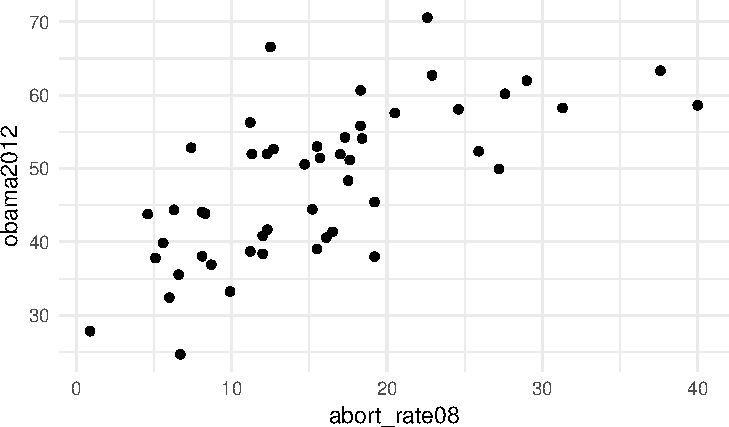
\includegraphics{qpolr_files/figure-latex/unnamed-chunk-170-1} \end{center}
  
  The colours are very bright. If we want to make them less so we can add
  \texttt{alpha} to \texttt{geom\_point()} to add transparency to the
  points. Below we use an alpha of 0.7 (if we want more transparency we
  can use a lower alpha level).
  \begin{Shaded}
  \begin{Highlighting}[]
  \KeywordTok{ggplot}\NormalTok{(states, }\KeywordTok{aes}\NormalTok{(}\DataTypeTok{x=}\NormalTok{abort_rate08, }\DataTypeTok{y=}\NormalTok{obama2012)) }\OperatorTok{+}
  \StringTok{  }\KeywordTok{geom_point}\NormalTok{(}\KeywordTok{aes}\NormalTok{(}\DataTypeTok{colour=}\NormalTok{abortlaw3), }\DataTypeTok{alpha=}\FloatTok{0.7}\NormalTok{) }\OperatorTok{+}\StringTok{ }
  \StringTok{  }\KeywordTok{geom_smooth}\NormalTok{(}\DataTypeTok{se=}\OtherTok{FALSE}\NormalTok{, }\DataTypeTok{colour=}\StringTok{"black"}\NormalTok{) }\OperatorTok{+}
  \StringTok{  }\KeywordTok{theme_minimal}\NormalTok{() }\OperatorTok{+}
  \StringTok{  }\KeywordTok{scale_colour_manual}\NormalTok{(}\DataTypeTok{values =} \KeywordTok{c}\NormalTok{(}\StringTok{"red"}\NormalTok{, }\StringTok{"blue"}\NormalTok{, }\StringTok{"black"}\NormalTok{)) }
  \end{Highlighting}
  \end{Shaded}
  \begin{center}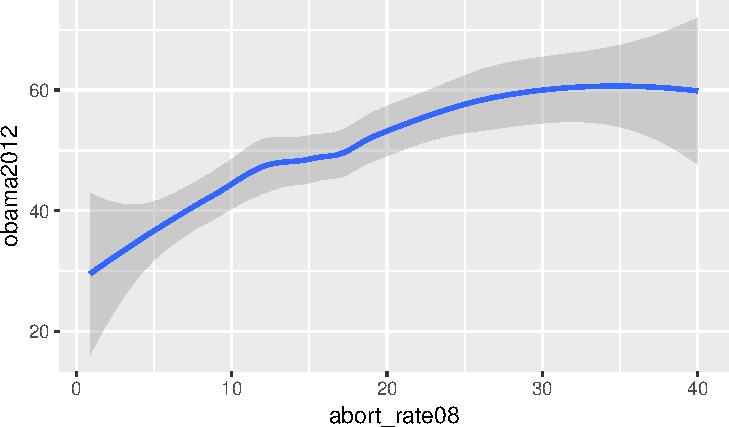
\includegraphics{qpolr_files/figure-latex/unnamed-chunk-171-1} \end{center}
  
  \subsection{Labels}\label{labels}
  
  Make sure that your figure have labels that helps the reader understand
  what is going on. To do this, you can add \texttt{labs()} to your
  figure. Here we will add a title, subtitle and caption.
  \begin{Shaded}
  \begin{Highlighting}[]
  \KeywordTok{ggplot}\NormalTok{(states, }\KeywordTok{aes}\NormalTok{(}\DataTypeTok{x=}\NormalTok{abort_rate08, }\DataTypeTok{y=}\NormalTok{obama2012)) }\OperatorTok{+}
  \StringTok{  }\KeywordTok{geom_point}\NormalTok{(}\KeywordTok{aes}\NormalTok{(}\DataTypeTok{colour=}\NormalTok{abortlaw3), }\DataTypeTok{alpha=}\FloatTok{0.7}\NormalTok{) }\OperatorTok{+}\StringTok{ }
  \StringTok{  }\KeywordTok{geom_smooth}\NormalTok{(}\DataTypeTok{se=}\OtherTok{FALSE}\NormalTok{, }\DataTypeTok{colour=}\StringTok{"black"}\NormalTok{) }\OperatorTok{+}
  \StringTok{  }\KeywordTok{theme_minimal}\NormalTok{() }\OperatorTok{+}
  \StringTok{  }\KeywordTok{scale_colour_manual}\NormalTok{(}\DataTypeTok{values =} \KeywordTok{c}\NormalTok{(}\StringTok{"red"}\NormalTok{, }\StringTok{"blue"}\NormalTok{, }\StringTok{"black"}\NormalTok{)) }\OperatorTok{+}
  \StringTok{  }\KeywordTok{labs}\NormalTok{(}
      \DataTypeTok{title =} \StringTok{"Abortion and the Obama vote"}\NormalTok{,}
      \DataTypeTok{subtitle =} \StringTok{"The relation between number of abortions and vote share for Obama"}\NormalTok{,}
      \DataTypeTok{caption =} \StringTok{"Data from the poliscidata R package"}\NormalTok{,}
      \DataTypeTok{colour =} \StringTok{"Abortion restrictions"}
  \NormalTok{  ) }
  \end{Highlighting}
  \end{Shaded}
  \begin{center}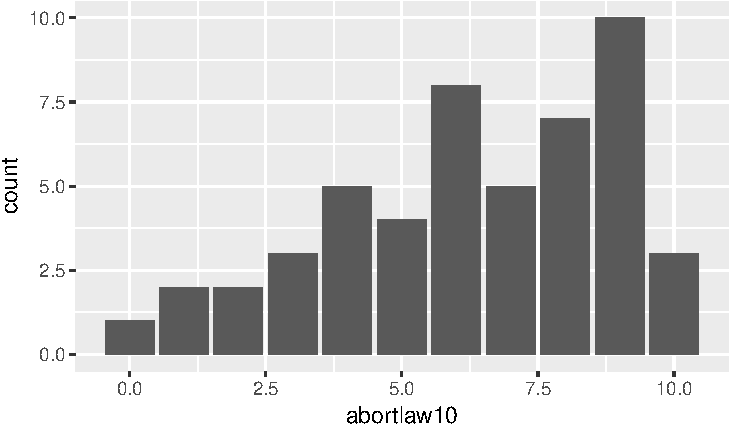
\includegraphics{qpolr_files/figure-latex/unnamed-chunk-172-1} \end{center}
  
  Last, we can see that the legend title is \texttt{abortlaw3}. We can
  change this by adding \texttt{colour} to \texttt{labs()} as well.
  \begin{Shaded}
  \begin{Highlighting}[]
  \KeywordTok{ggplot}\NormalTok{(states, }\KeywordTok{aes}\NormalTok{(}\DataTypeTok{x=}\NormalTok{abort_rate08, }\DataTypeTok{y=}\NormalTok{obama2012)) }\OperatorTok{+}
  \StringTok{  }\KeywordTok{geom_point}\NormalTok{(}\KeywordTok{aes}\NormalTok{(}\DataTypeTok{colour=}\NormalTok{abortlaw3), }\DataTypeTok{alpha=}\FloatTok{0.7}\NormalTok{) }\OperatorTok{+}\StringTok{ }
  \StringTok{  }\KeywordTok{geom_smooth}\NormalTok{(}\DataTypeTok{se=}\OtherTok{FALSE}\NormalTok{, }\DataTypeTok{colour=}\StringTok{"black"}\NormalTok{) }\OperatorTok{+}
  \StringTok{  }\KeywordTok{theme_minimal}\NormalTok{() }\OperatorTok{+}
  \StringTok{  }\KeywordTok{scale_colour_manual}\NormalTok{(}\DataTypeTok{values =} \KeywordTok{c}\NormalTok{(}\StringTok{"red"}\NormalTok{, }\StringTok{"blue"}\NormalTok{, }\StringTok{"black"}\NormalTok{)) }\OperatorTok{+}
  \StringTok{  }\KeywordTok{labs}\NormalTok{(}
      \DataTypeTok{title =} \StringTok{"Abortion and the Obama vote"}\NormalTok{,}
      \DataTypeTok{subtitle =} \StringTok{"The relation between number of abortions and vote share for Obama"}\NormalTok{,}
      \DataTypeTok{caption =} \StringTok{"Data from the poliscidata R package"}\NormalTok{,}
      \DataTypeTok{colour =} \StringTok{"Abortion restrictions"}
  \NormalTok{  ) }
  \end{Highlighting}
  \end{Shaded}
  \begin{center}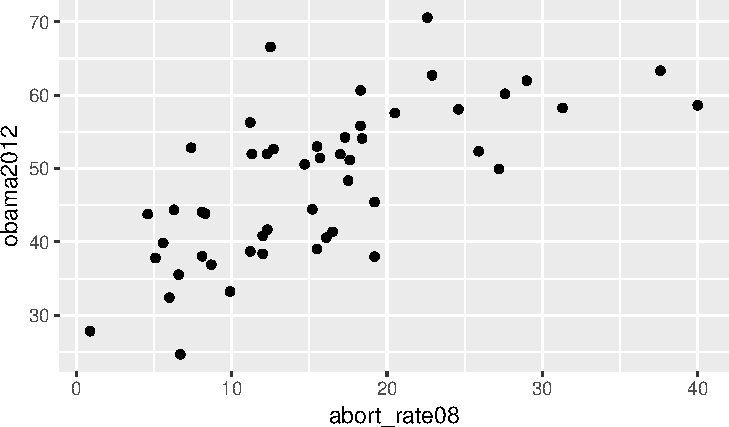
\includegraphics{qpolr_files/figure-latex/unnamed-chunk-173-1} \end{center}
  
  \subsection{Axes}\label{axes}
  
  Related to labels are the axes. Always label the axes so they have
  meaningful names. The variable name is not a meaningful name. We add
  \texttt{x} and \texttt{y} to the \texttt{labs()} addition in our plot.
  \begin{Shaded}
  \begin{Highlighting}[]
  \KeywordTok{ggplot}\NormalTok{(states, }\KeywordTok{aes}\NormalTok{(}\DataTypeTok{x=}\NormalTok{abort_rate08, }\DataTypeTok{y=}\NormalTok{obama2012)) }\OperatorTok{+}
  \StringTok{  }\KeywordTok{geom_point}\NormalTok{(}\KeywordTok{aes}\NormalTok{(}\DataTypeTok{colour=}\NormalTok{abortlaw3), }\DataTypeTok{alpha=}\FloatTok{0.7}\NormalTok{) }\OperatorTok{+}\StringTok{ }
  \StringTok{  }\KeywordTok{geom_smooth}\NormalTok{(}\DataTypeTok{se=}\OtherTok{FALSE}\NormalTok{, }\DataTypeTok{colour=}\StringTok{"black"}\NormalTok{) }\OperatorTok{+}
  \StringTok{  }\KeywordTok{theme_minimal}\NormalTok{() }\OperatorTok{+}
  \StringTok{  }\KeywordTok{scale_colour_manual}\NormalTok{(}\DataTypeTok{values =} \KeywordTok{c}\NormalTok{(}\StringTok{"red"}\NormalTok{, }\StringTok{"blue"}\NormalTok{, }\StringTok{"black"}\NormalTok{)) }\OperatorTok{+}
  \StringTok{  }\KeywordTok{labs}\NormalTok{(}
      \DataTypeTok{title =} \StringTok{"Abortion and the Obama vote"}\NormalTok{,}
      \DataTypeTok{subtitle =} \StringTok{"The relation between number of abortions and vote share for Obama"}\NormalTok{,}
      \DataTypeTok{caption =} \StringTok{"Data from the poliscidata R package"}\NormalTok{,}
      \DataTypeTok{colour =} \StringTok{"Abortion restrictions"}\NormalTok{,}
      \DataTypeTok{y =} \StringTok{"Obama vote share in 2012"}\NormalTok{,}
      \DataTypeTok{x =} \StringTok{"Number of abortions per 1,000 women aged 15-44 in 2008"}
  \NormalTok{  ) }
  \end{Highlighting}
  \end{Shaded}
  \begin{center}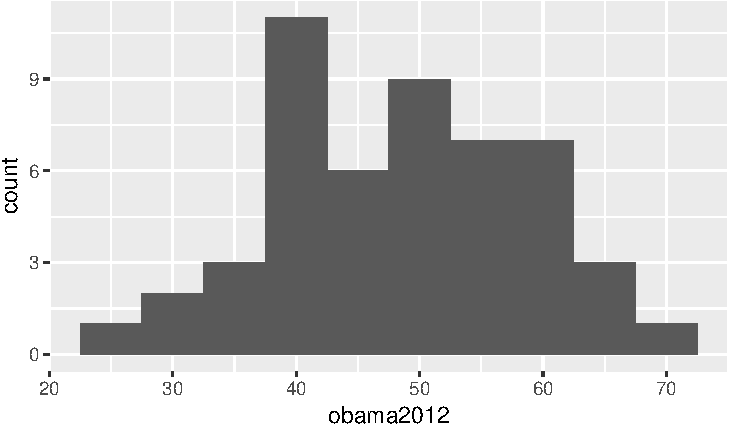
\includegraphics{qpolr_files/figure-latex/unnamed-chunk-174-1} \end{center}
  
  \subsection{Confidence intervals}\label{confidence-intervals}
  
  We can have confidence intervals in our figure by not having \texttt{se}
  (standard errors) set to \texttt{FALSE}.
  \begin{Shaded}
  \begin{Highlighting}[]
  \KeywordTok{ggplot}\NormalTok{(states, }\KeywordTok{aes}\NormalTok{(}\DataTypeTok{x=}\NormalTok{abort_rate08, }\DataTypeTok{y=}\NormalTok{obama2012)) }\OperatorTok{+}
  \StringTok{  }\KeywordTok{geom_point}\NormalTok{(}\KeywordTok{aes}\NormalTok{(}\DataTypeTok{colour=}\NormalTok{abortlaw3), }\DataTypeTok{alpha=}\FloatTok{0.7}\NormalTok{) }\OperatorTok{+}\StringTok{ }
  \StringTok{  }\KeywordTok{geom_smooth}\NormalTok{(}\DataTypeTok{colour=}\StringTok{"black"}\NormalTok{) }\OperatorTok{+}
  \StringTok{  }\KeywordTok{theme_minimal}\NormalTok{() }\OperatorTok{+}
  \StringTok{  }\KeywordTok{scale_colour_manual}\NormalTok{(}\DataTypeTok{values =} \KeywordTok{c}\NormalTok{(}\StringTok{"red"}\NormalTok{, }\StringTok{"blue"}\NormalTok{, }\StringTok{"black"}\NormalTok{)) }\OperatorTok{+}
  \StringTok{  }\KeywordTok{labs}\NormalTok{(}
      \DataTypeTok{title =} \StringTok{"Abortion and the Obama vote"}\NormalTok{,}
      \DataTypeTok{subtitle =} \StringTok{"The relation between number of abortions and vote share for Obama"}\NormalTok{,}
      \DataTypeTok{caption =} \StringTok{"Data from the poliscidata R package"}\NormalTok{,}
      \DataTypeTok{colour =} \StringTok{"Abortion restrictions"}\NormalTok{,}
      \DataTypeTok{y =} \StringTok{"Obama vote share in 2012"}\NormalTok{,}
      \DataTypeTok{x =} \StringTok{"Number of abortions per 1,000 women aged 15-44 in 2008"}
  \NormalTok{  ) }
  \end{Highlighting}
  \end{Shaded}
  \begin{center}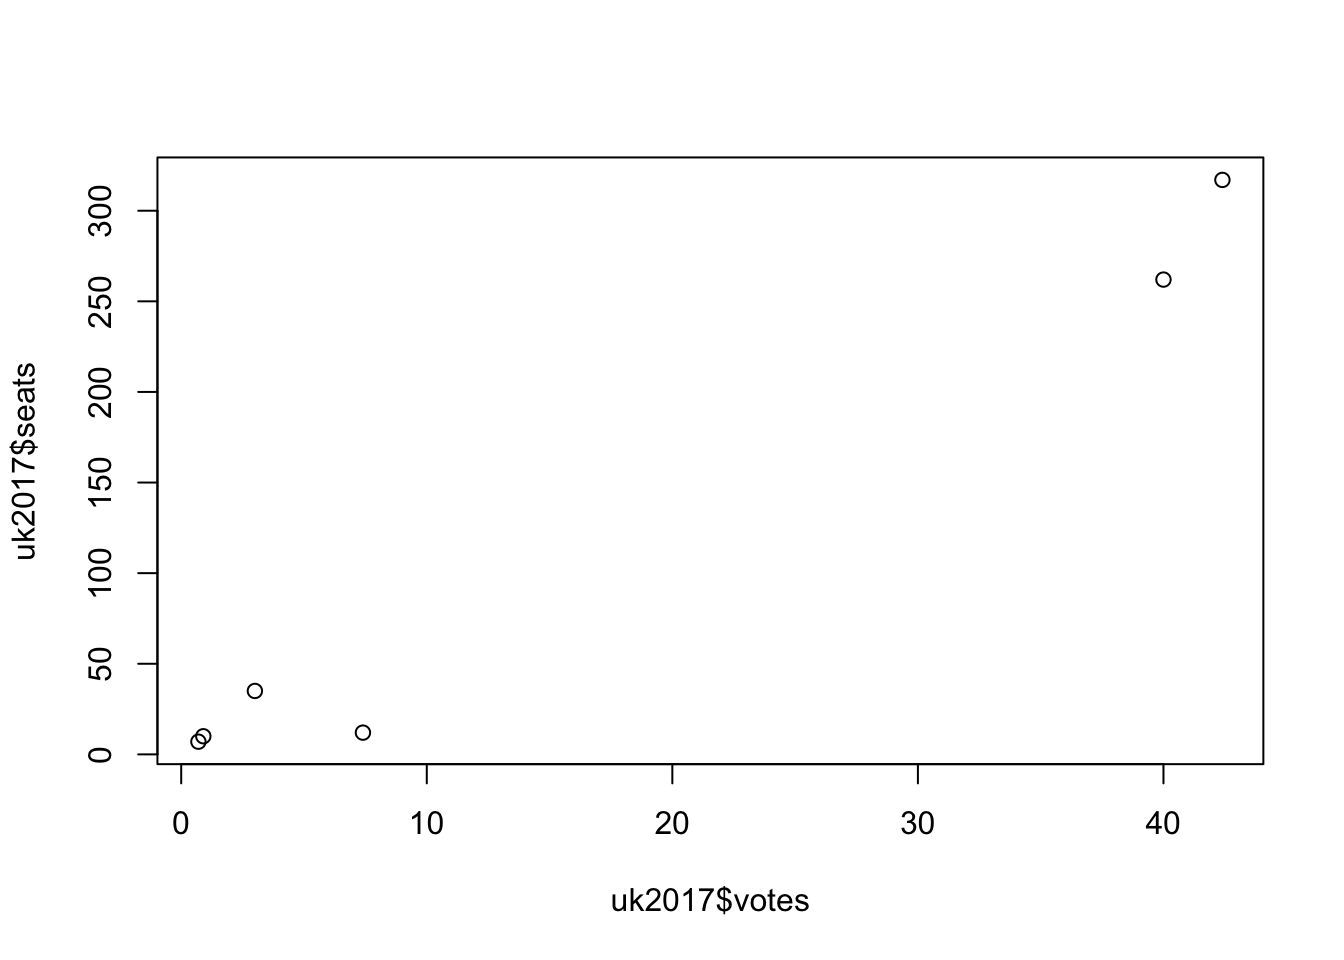
\includegraphics{qpolr_files/figure-latex/unnamed-chunk-175-1} \end{center}
  
  \subsection{Making multiple plots in
  one}\label{making-multiple-plots-in-one}
  
  If we would prefer to have the plots for different observations, we can
  specify that with \texttt{facet\_grid()}.
  \begin{Shaded}
  \begin{Highlighting}[]
  \KeywordTok{ggplot}\NormalTok{(states, }\KeywordTok{aes}\NormalTok{(}\DataTypeTok{x=}\NormalTok{abort_rate08, }\DataTypeTok{y=}\NormalTok{obama2012)) }\OperatorTok{+}
  \StringTok{  }\KeywordTok{geom_point}\NormalTok{(}\KeywordTok{aes}\NormalTok{(}\DataTypeTok{colour=}\NormalTok{abortlaw3), }\DataTypeTok{alpha=}\FloatTok{0.7}\NormalTok{) }\OperatorTok{+}\StringTok{ }
  \StringTok{  }\KeywordTok{geom_smooth}\NormalTok{(}\DataTypeTok{colour=}\StringTok{"black"}\NormalTok{) }\OperatorTok{+}
  \StringTok{  }\KeywordTok{theme_minimal}\NormalTok{() }\OperatorTok{+}
  \StringTok{  }\KeywordTok{scale_colour_manual}\NormalTok{(}\DataTypeTok{values =} \KeywordTok{c}\NormalTok{(}\StringTok{"red"}\NormalTok{, }\StringTok{"blue"}\NormalTok{, }\StringTok{"black"}\NormalTok{)) }\OperatorTok{+}
  \StringTok{  }\KeywordTok{labs}\NormalTok{(}
      \DataTypeTok{title =} \StringTok{"Abortion and the Obama vote"}\NormalTok{,}
      \DataTypeTok{subtitle =} \StringTok{"The relation between number of abortions and vote share for Obama"}\NormalTok{,}
      \DataTypeTok{caption =} \StringTok{"Data from the poliscidata R package"}\NormalTok{,}
      \DataTypeTok{colour =} \StringTok{"Abortion restrictions"}\NormalTok{,}
      \DataTypeTok{y =} \StringTok{"Obama vote share in 2012"}\NormalTok{,}
      \DataTypeTok{x =} \StringTok{"Number of abortions per 1,000 women aged 15-44 in 2008"}
  \NormalTok{  ) }\OperatorTok{+}
  \StringTok{  }\KeywordTok{facet_grid}\NormalTok{(}\OperatorTok{~}\StringTok{ }\NormalTok{abortlaw3)}
  \end{Highlighting}
  \end{Shaded}
  \begin{center}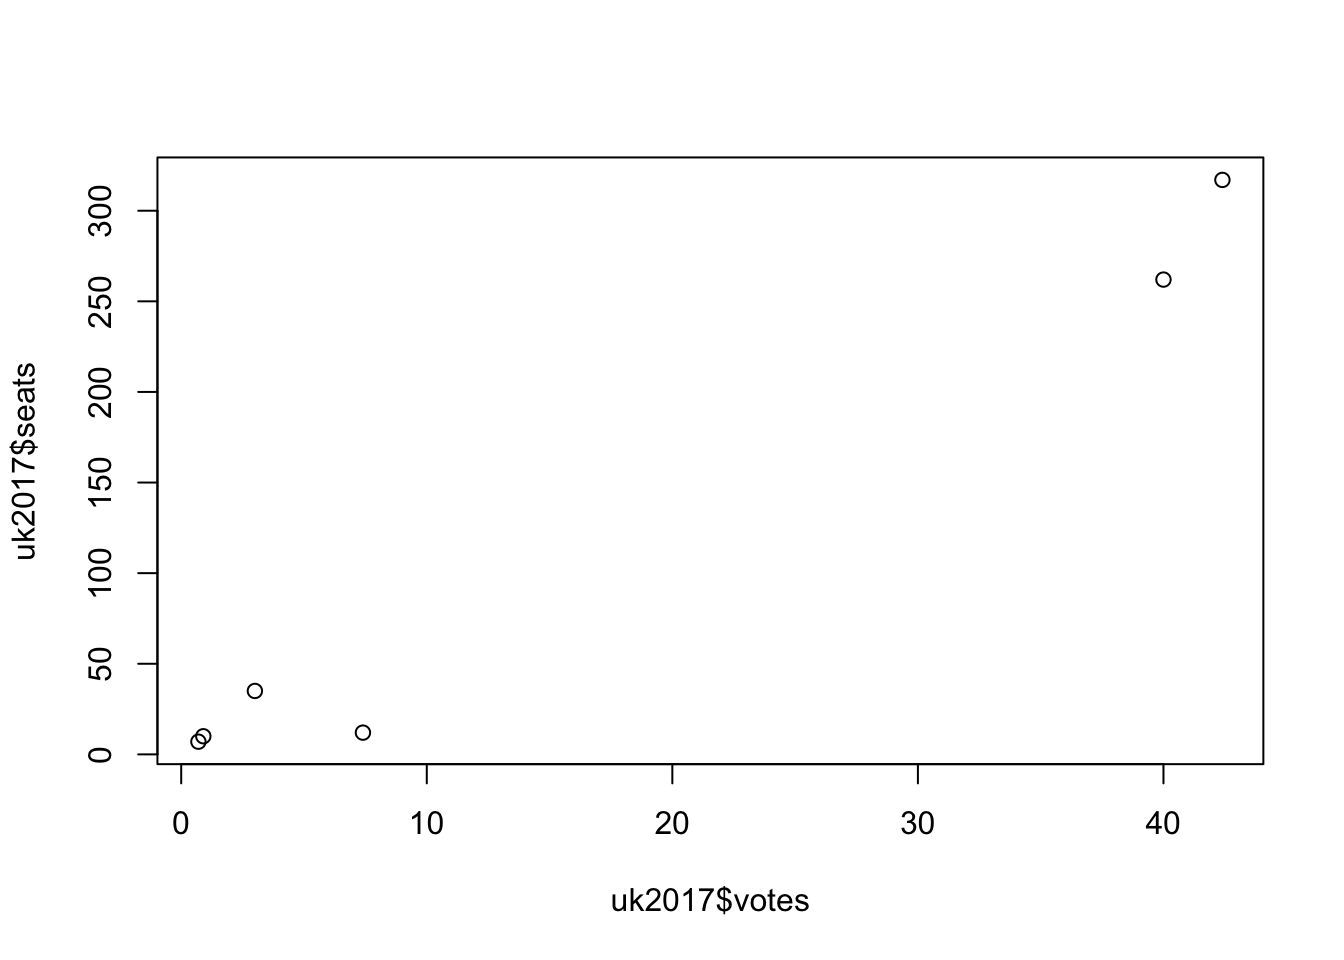
\includegraphics{qpolr_files/figure-latex/unnamed-chunk-176-1} \end{center}
  
  \section{Saving plots}\label{saving-plots}
  
  When you have a plot you would like to save, you can use
  \texttt{ggsave()}. Do keep in mind that it will only save the last plot
  you have created.
  \begin{Shaded}
  \begin{Highlighting}[]
  \KeywordTok{ggsave}\NormalTok{(}\StringTok{"fig1-abortion.png"}\NormalTok{)}
  \end{Highlighting}
  \end{Shaded}
  The figure will be saved in your working directory. The file type
  \texttt{.png} can be replaced to whatever format you would prefer your
  figure to be in. If you have saved your figure in an object, you can
  save it by specifying this before the file name.
  \begin{Shaded}
  \begin{Highlighting}[]
  \KeywordTok{ggsave}\NormalTok{(fig1, }\StringTok{"fig1-abortion.png"}\NormalTok{)}
  \end{Highlighting}
  \end{Shaded}
  Often you will see that you are not totally satisfied with the size of
  your figure. To change this, you can use \texttt{width} and
  \texttt{height}.
  \begin{Shaded}
  \begin{Highlighting}[]
  \KeywordTok{ggsave}\NormalTok{(fig1, }\StringTok{"fig1-abortion.png"}\NormalTok{, }\DataTypeTok{width =} \DecValTok{4}\NormalTok{, }\DataTypeTok{height =} \DecValTok{4}\NormalTok{)}
  \end{Highlighting}
  \end{Shaded}
  \chapter*{(PART) Regression}\label{part-regression}
  \addcontentsline{toc}{chapter}{(PART) Regression}
  
  \chapter{OLS regression}\label{olsreg}
  
  To provide a simple example of how to conduct an OLS regression, we will
  use the same data as in the visualisation chapter, i.e.~the
  \texttt{states} data frame from the package \texttt{poliscidata}.
  \begin{Shaded}
  \begin{Highlighting}[]
  \KeywordTok{library}\NormalTok{(}\StringTok{"poliscidata"}\NormalTok{)}
  
  \NormalTok{states <-}\StringTok{ }\NormalTok{states}
  \end{Highlighting}
  \end{Shaded}
  \section{Bivariate linear regression}\label{bivariate-linear-regression}
  
  To conduct a bivariate linear regression, we use the \texttt{lm()}
  function (short for linear models). We need to specify the dependent
  variable, independent variable and the data frame. Below we specify
  \texttt{obama2012} as the dependent variable and \texttt{abort\_rate08}
  as the independent variable. Notice that we use the
  \texttt{\textasciitilde{}} symbol to separate the dependent variable
  from the independent variable. We save the output in the object
  \texttt{reg\_obama}.
  \begin{Shaded}
  \begin{Highlighting}[]
  \NormalTok{reg_obama <-}\StringTok{ }\KeywordTok{lm}\NormalTok{(obama2012 }\OperatorTok{~}\StringTok{ }\NormalTok{abort_rate08, }\DataTypeTok{data =}\NormalTok{ states)}
  \end{Highlighting}
  \end{Shaded}
  If we type \texttt{reg\_obama}, we can see the intercept and coefficient
  in the model.
  \begin{Shaded}
  \begin{Highlighting}[]
  \NormalTok{reg_obama}
  \end{Highlighting}
  \end{Shaded}
  \begin{verbatim}
  
  Call:
  lm(formula = obama2012 ~ abort_rate08, data = states)
  
  Coefficients:
   (Intercept)  abort_rate08  
       35.2589        0.8257  
  \end{verbatim}
  Here we see that the intercept is 35.26, which is the predicted vote
  share for Obama in 2012 when we extrapolate to a state with an abortion
  rate of 0. The coefficient is 0.83, which is the increase in the vote
  share for Obama when there is an one-unit increase in the abortion rate.
  
  However, this is not enough information. We need, for example, also
  information on the standard errors as well as model statistics. To get
  this, we use the function \texttt{summary()} on our object.
  \begin{Shaded}
  \begin{Highlighting}[]
  \KeywordTok{summary}\NormalTok{(reg_obama)}
  \end{Highlighting}
  \end{Shaded}
  \begin{verbatim}
  
  Call:
  lm(formula = obama2012 ~ abort_rate08, data = states)
  
  Residuals:
       Min       1Q   Median       3Q      Max 
  -16.1208  -5.6516   0.6785   4.7242  20.9904 
  
  Coefficients:
               Estimate Std. Error t value Pr(>|t|)    
  (Intercept)   35.2589     2.2970  15.350  < 2e-16 ***
  abort_rate08   0.8257     0.1297   6.366 6.91e-08 ***
  ---
  Signif. codes:  0 '***' 0.001 '**' 0.01 '*' 0.05 '.' 0.1 ' ' 1
  
  Residual standard error: 7.654 on 48 degrees of freedom
  Multiple R-squared:  0.4578,    Adjusted R-squared:  0.4465 
  F-statistic: 40.52 on 1 and 48 DF,  p-value: 6.912e-08
  \end{verbatim}
  Here we can see that the estimate for \texttt{abort\_rate08} is
  statistically significant. We can further see that the R-squared is 0.46
  which indicates that 46\% of the variation in the vote share is
  explained by our independent variable.
  
  To convert the results from our analysis into a data frame, we can use
  the package \texttt{broom} (Robinson, 2018).
  \begin{Shaded}
  \begin{Highlighting}[]
  \KeywordTok{library}\NormalTok{(}\StringTok{"broom"}\NormalTok{)}
  \end{Highlighting}
  \end{Shaded}
  As a first example, we can save the estimates and test statistics in a
  data frame by using the function \texttt{tidy()}. We save the output in
  a new object \texttt{reg\_obama\_tidy} and show this output as well.
  \begin{Shaded}
  \begin{Highlighting}[]
  \NormalTok{reg_obama_tidy <-}\StringTok{ }\KeywordTok{tidy}\NormalTok{(reg_obama)}
  
  \NormalTok{reg_obama_tidy}
  \end{Highlighting}
  \end{Shaded}
  \begin{verbatim}
            term  estimate std.error statistic      p.value
  1  (Intercept) 35.258869 2.2970329 15.349745 3.818291e-20
  2 abort_rate08  0.825655 0.1297048  6.365649 6.911913e-08
  \end{verbatim}
  If we would also like to have the confidence intervals, we can add the
  \texttt{conf.int\ =\ TRUE}.
  \begin{Shaded}
  \begin{Highlighting}[]
  \NormalTok{reg_obama_tidy <-}\StringTok{ }\KeywordTok{tidy}\NormalTok{(reg_obama, }\DataTypeTok{conf.int =} \OtherTok{TRUE}\NormalTok{)}
  
  \NormalTok{reg_obama_tidy}
  \end{Highlighting}
  \end{Shaded}
  \begin{verbatim}
            term  estimate std.error statistic      p.value   conf.low
  1  (Intercept) 35.258869 2.2970329 15.349745 3.818291e-20 30.6403753
  2 abort_rate08  0.825655 0.1297048  6.365649 6.911913e-08  0.5648661
    conf.high
  1 39.877364
  2  1.086444
  \end{verbatim}
  This is useful if you would like to visualise the results. However,
  often we also want to save predictions and residuals based on our model.
  To do this, we can use the function \texttt{augment()}. Below we save
  the output in the object \texttt{reg\_obama\_aug}.
  \begin{Shaded}
  \begin{Highlighting}[]
  \NormalTok{reg_obama_aug <-}\StringTok{ }\KeywordTok{augment}\NormalTok{(reg_obama)}
  \end{Highlighting}
  \end{Shaded}
  To see the data in the new object, use \texttt{head()}. Here you see
  that there is a variable called \texttt{.fitted}. This variable is the
  predicted value for each observation.
  \begin{Shaded}
  \begin{Highlighting}[]
  \KeywordTok{head}\NormalTok{(reg_obama_aug)}
  \end{Highlighting}
  \end{Shaded}
  \begin{verbatim}
    obama2012 abort_rate08  .fitted  .se.fit    .resid       .hat   .sigma
  1     40.81         12.0 45.16673 1.179911 -4.356729 0.02376297 7.708398
  2     38.36         12.0 45.16673 1.179911 -6.806729 0.02376297 7.669635
  3     36.88          8.7 42.44207 1.406179 -5.562068 0.03375074 7.691025
  4     44.45         15.2 47.80882 1.083835 -3.358825 0.02005065 7.719335
  5     60.19         27.6 58.04695 1.893732  2.143053 0.06121236 7.728453
  6     51.45         15.7 48.22165 1.082515  3.228348 0.02000184 7.720544
        .cooksd .std.resid
  1 0.004039088 -0.5760815
  2 0.009859143 -0.9000401
  3 0.009544419 -0.7392523
  4 0.002010333 -0.4432886
  5 0.002722341  0.2889684
  6 0.001852473  0.4260579
  \end{verbatim}
  We can use this data frame to visualise the residuals (with the colour
  red below).
  \begin{Shaded}
  \begin{Highlighting}[]
  \KeywordTok{ggplot}\NormalTok{(reg_obama_aug, }\KeywordTok{aes}\NormalTok{(}\DataTypeTok{x=}\NormalTok{abort_rate08, }\DataTypeTok{y=}\NormalTok{obama2012)) }\OperatorTok{+}
  \StringTok{  }\KeywordTok{geom_segment}\NormalTok{(}\KeywordTok{aes}\NormalTok{(}\DataTypeTok{xend=}\NormalTok{abort_rate08, }\DataTypeTok{y=}\NormalTok{obama2012, }\DataTypeTok{yend=}\NormalTok{.fitted), }
          \DataTypeTok{colour=}\StringTok{"red"}\NormalTok{) }\OperatorTok{+}
  \StringTok{  }\KeywordTok{geom_point}\NormalTok{() }\OperatorTok{+}
  \StringTok{  }\KeywordTok{geom_line}\NormalTok{(}\KeywordTok{aes}\NormalTok{(}\DataTypeTok{x=}\NormalTok{abort_rate08, }\DataTypeTok{y=}\NormalTok{.fitted)) }
  \end{Highlighting}
  \end{Shaded}
  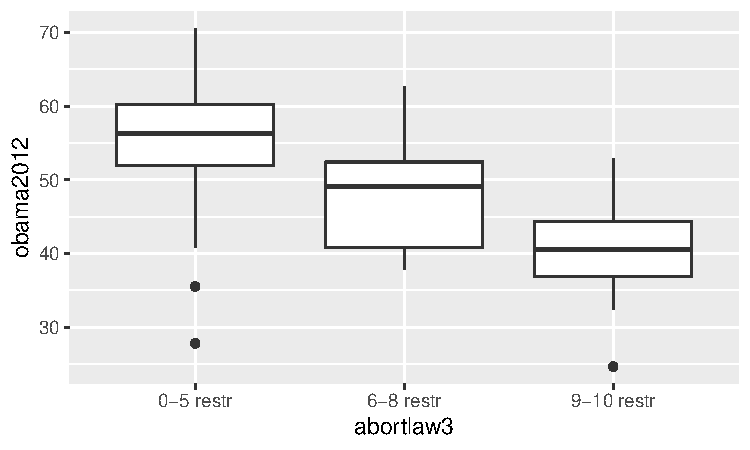
\includegraphics{qpolr_files/figure-latex/unnamed-chunk-189-1.pdf}
  
  \section{Multiple linear regression}\label{multiple-linear-regression}
  
  To conduct a multiple linear regression, we simply need to add an extra
  variable to our model. Accordingly, the only difference between the
  example above and the example here is the addition of a new variable.
  Here, we want to examine whether the effect of \texttt{abort\_rate08}
  holds when we control for population density (\texttt{density}). Notice
  that we add a \texttt{+} before adding the variable to the list of
  variables.
  \begin{Shaded}
  \begin{Highlighting}[]
  \NormalTok{reg_obama_full <-}\StringTok{ }\KeywordTok{lm}\NormalTok{(obama2012 }\OperatorTok{~}\StringTok{ }\NormalTok{abort_rate08 }\OperatorTok{+}\StringTok{ }\NormalTok{density, }\DataTypeTok{data =}\NormalTok{ states)}
  \end{Highlighting}
  \end{Shaded}
  We use the \texttt{summary()} function to get the output of the model.
  \begin{Shaded}
  \begin{Highlighting}[]
  \KeywordTok{summary}\NormalTok{(reg_obama_full)}
  \end{Highlighting}
  \end{Shaded}
  \begin{verbatim}
  
  Call:
  lm(formula = obama2012 ~ abort_rate08 + density, data = states)
  
  Residuals:
       Min       1Q   Median       3Q      Max 
  -16.1719  -5.5567  -0.2101   4.3195  21.5132 
  
  Coefficients:
                Estimate Std. Error t value Pr(>|t|)    
  (Intercept)  36.019160   2.328169  15.471  < 2e-16 ***
  abort_rate08  0.681420   0.161482   4.220 0.000111 ***
  density       0.007656   0.005214   1.468 0.148669    
  ---
  Signif. codes:  0 '***' 0.001 '**' 0.01 '*' 0.05 '.' 0.1 ' ' 1
  
  Residual standard error: 7.564 on 47 degrees of freedom
  Multiple R-squared:  0.4815,    Adjusted R-squared:  0.4595 
  F-statistic: 21.83 on 2 and 47 DF,  p-value: 1.976e-07
  \end{verbatim}
  In the output we see that the coefficient for \texttt{abort\_rate08} is
  slightly smaller compared to the bivariate model but still statistically
  significant. Again we can use the \texttt{tidy()} function to get a data
  frame with the results.
  \begin{Shaded}
  \begin{Highlighting}[]
  \NormalTok{reg_obama_full_tidy <-}\StringTok{ }\KeywordTok{tidy}\NormalTok{(reg_obama_full)}
  \end{Highlighting}
  \end{Shaded}
  We further calculate the 95\% confidence intervals for the estimates.
  \begin{Shaded}
  \begin{Highlighting}[]
  \NormalTok{reg_obama_full_tidy <-}\StringTok{ }\NormalTok{reg_obama_full_tidy }\OperatorTok
  \StringTok{  }\KeywordTok{mutate}\NormalTok{(}
      \DataTypeTok{ci_low =}\NormalTok{ estimate }\OperatorTok{-}\StringTok{ }\FloatTok{1.96} \OperatorTok{*}\StringTok{ }\NormalTok{std.error,}
      \DataTypeTok{ci_high =}\NormalTok{ estimate }\OperatorTok{+}\StringTok{ }\FloatTok{1.96} \OperatorTok{*}\StringTok{ }\NormalTok{std.error}
  \NormalTok{  ) }
  \end{Highlighting}
  \end{Shaded}
  We can then visualise the results.
  \begin{Shaded}
  \begin{Highlighting}[]
  \KeywordTok{ggplot}\NormalTok{(reg_obama_full_tidy, }\KeywordTok{aes}\NormalTok{(estimate, term, }\DataTypeTok{xmin =}\NormalTok{ ci_low, }
                                  \DataTypeTok{xmax =}\NormalTok{ ci_high, }\DataTypeTok{height =} \DecValTok{0}\NormalTok{)) }\OperatorTok{+}
  \StringTok{     }\KeywordTok{geom_point}\NormalTok{() }\OperatorTok{+}
  \StringTok{     }\KeywordTok{geom_vline}\NormalTok{(}\DataTypeTok{xintercept =} \DecValTok{0}\NormalTok{) }\OperatorTok{+}
  \StringTok{     }\KeywordTok{geom_errorbarh}\NormalTok{()}
  \end{Highlighting}
  \end{Shaded}
  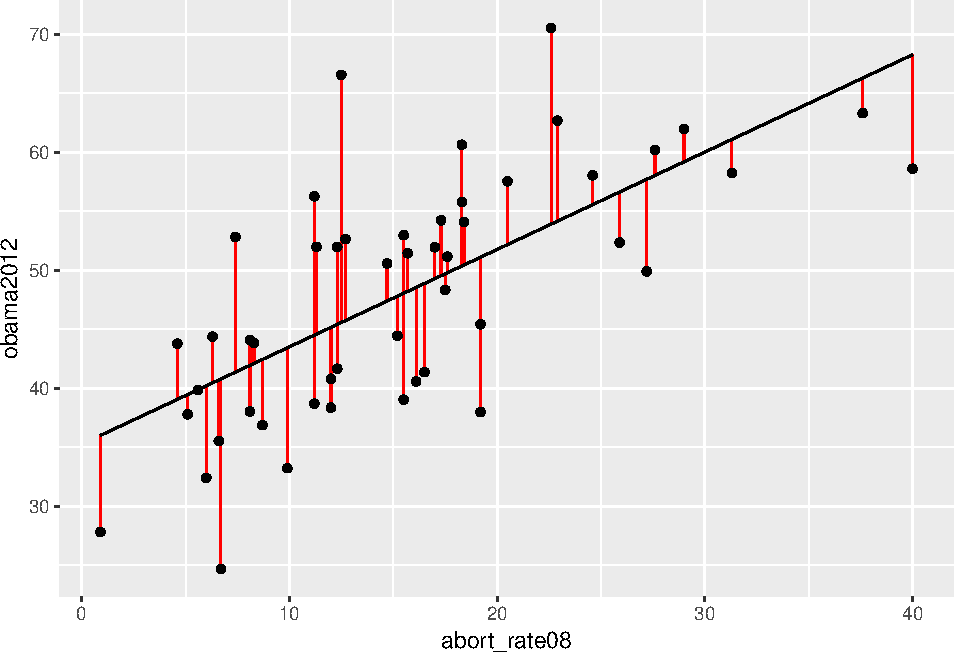
\includegraphics{qpolr_files/figure-latex/unnamed-chunk-194-1.pdf}
  
  In some cases the intercept is not relevant. In the code below, we use
  the \texttt{filter()} function to visualise all effects except for the
  intercept.
  \begin{Shaded}
  \begin{Highlighting}[]
  \NormalTok{reg_obama_full_tidy }\OperatorTok
  \StringTok{  }\KeywordTok{filter}\NormalTok{(term }\OperatorTok{!=}\StringTok{ "(Intercept)"}\NormalTok{) }\OperatorTok
  \StringTok{  }\KeywordTok{ggplot}\NormalTok{(}\KeywordTok{aes}\NormalTok{(estimate, term, }\DataTypeTok{xmin =}\NormalTok{ ci_low, }
               \DataTypeTok{xmax =}\NormalTok{ ci_high, }\DataTypeTok{height =} \DecValTok{0}\NormalTok{)) }\OperatorTok{+}
  \StringTok{     }\KeywordTok{geom_point}\NormalTok{() }\OperatorTok{+}
  \StringTok{     }\KeywordTok{geom_vline}\NormalTok{(}\DataTypeTok{xintercept =} \DecValTok{0}\NormalTok{) }\OperatorTok{+}
  \StringTok{     }\KeywordTok{geom_errorbarh}\NormalTok{()}
  \end{Highlighting}
  \end{Shaded}
  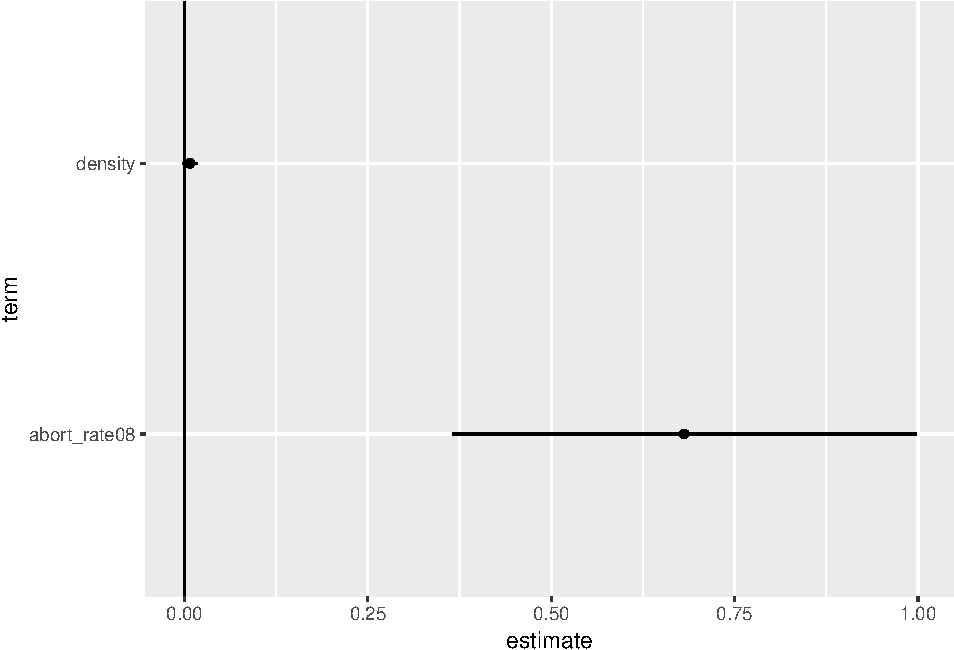
\includegraphics{qpolr_files/figure-latex/unnamed-chunk-195-1.pdf}
  
  \section{Diagnostic tests}\label{diagnostic-tests}
  
  To get diagnostic plots, we will use the \texttt{fortify()} function
  from \texttt{ggplot2}. This allows us to get the following variables
  realted to model fit statistics:
  \begin{enumerate}
  \def\labelenumi{\arabic{enumi}.}
  \tightlist
  \item
    \texttt{.hat}: Diagonal of the hat matrix
  \item
    \texttt{.sigma}: Estimate of residual standard deviation when
    corresponding observation is dropped from model
  \item
    \texttt{.cooksd}: Cooks distance, using \texttt{cooks.distance()}
  \item
    \texttt{.fitted}: Fitted values of model
  \item
    \texttt{.resid}: Residuals
  \item
    \texttt{.stdresid}: Standardised residuals
  \end{enumerate}
  First, we use \texttt{fortify()} on our linear model:
  \begin{Shaded}
  \begin{Highlighting}[]
  \NormalTok{reg_fortify <-}\StringTok{ }\KeywordTok{fortify}\NormalTok{(reg_obama_full)}
  \end{Highlighting}
  \end{Shaded}
  To see how our residuals are in relation to our fitted values, we can
  plot \texttt{.fitted} and \texttt{.resid}.
  \begin{Shaded}
  \begin{Highlighting}[]
  \KeywordTok{ggplot}\NormalTok{(reg_fortify, }\KeywordTok{aes}\NormalTok{(}\DataTypeTok{x =}\NormalTok{ .fitted, }\DataTypeTok{y =}\NormalTok{ .resid)) }\OperatorTok{+}
  \StringTok{  }\KeywordTok{geom_point}\NormalTok{() }\OperatorTok{+}
  \StringTok{  }\KeywordTok{geom_hline}\NormalTok{(}\DataTypeTok{yintercept =} \DecValTok{0}\NormalTok{) }\OperatorTok{+}
  \StringTok{  }\KeywordTok{geom_smooth}\NormalTok{(}\DataTypeTok{se =} \OtherTok{FALSE}\NormalTok{) }\OperatorTok{+}
  \StringTok{  }\KeywordTok{labs}\NormalTok{(}\DataTypeTok{title =} \StringTok{"Residuals vs. Fitted"}\NormalTok{,}
         \DataTypeTok{y =} \StringTok{"Residuals"}\NormalTok{,}
         \DataTypeTok{x =} \StringTok{"Fitted values"}\NormalTok{)}
  \end{Highlighting}
  \end{Shaded}
  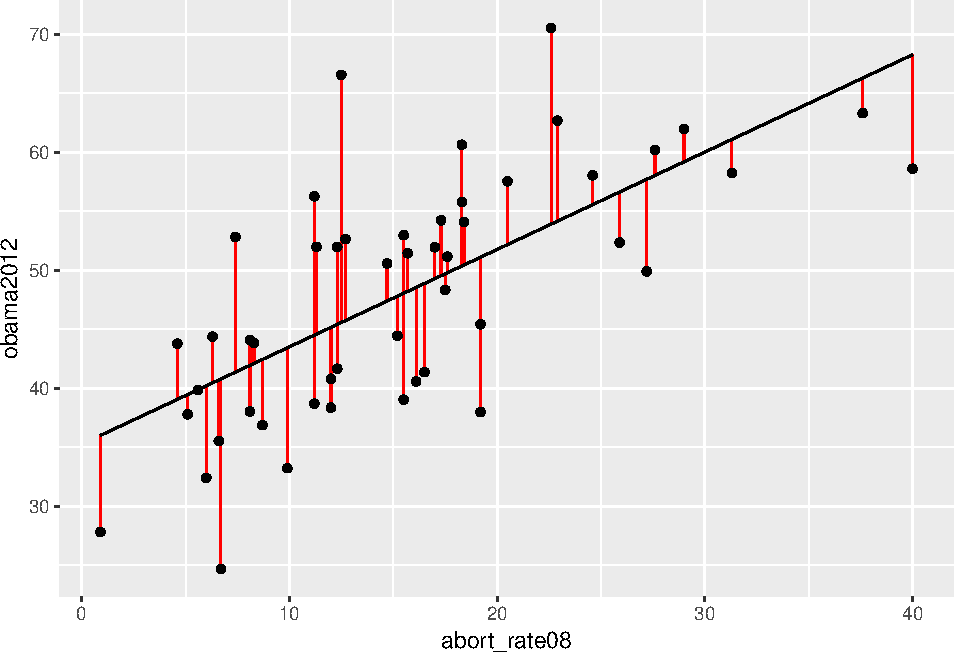
\includegraphics{qpolr_files/figure-latex/unnamed-chunk-197-1.pdf}
  
  To see whether our residuals are normally distributed, we create a
  normal Q-Q plot with the standardized residuals.
  \begin{Shaded}
  \begin{Highlighting}[]
  \KeywordTok{ggplot}\NormalTok{(reg_fortify) }\OperatorTok{+}
  \StringTok{  }\KeywordTok{stat_qq}\NormalTok{(}\KeywordTok{aes}\NormalTok{(}\DataTypeTok{sample =}\NormalTok{ .stdresid)) }\OperatorTok{+}
  \StringTok{  }\KeywordTok{geom_abline}\NormalTok{() }\OperatorTok{+}
  \StringTok{  }\KeywordTok{labs}\NormalTok{(}\DataTypeTok{title =} \StringTok{"Normal Q-Q"}\NormalTok{,}
         \DataTypeTok{y =} \StringTok{"Standardized residuals"}\NormalTok{,}
         \DataTypeTok{x =} \StringTok{"Theoretical Quantiles"}\NormalTok{)}
  \end{Highlighting}
  \end{Shaded}
  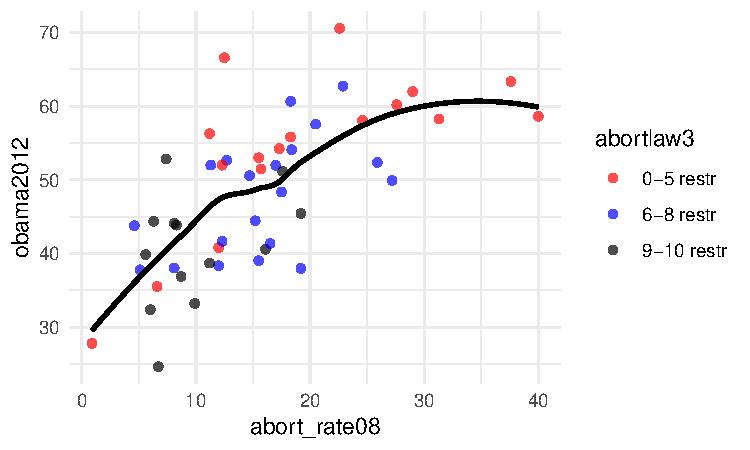
\includegraphics{qpolr_files/figure-latex/unnamed-chunk-198-1.pdf}
  
  To estimate the influence of individual observations, we plot the Cook's
  distance for each state.
  \begin{Shaded}
  \begin{Highlighting}[]
  \KeywordTok{ggplot}\NormalTok{(reg_fortify, }\KeywordTok{aes}\NormalTok{(}\DataTypeTok{x =} \KeywordTok{seq_along}\NormalTok{(.cooksd), }\DataTypeTok{y =}\NormalTok{ .cooksd)) }\OperatorTok{+}
  \StringTok{  }\KeywordTok{geom_col}\NormalTok{()  }\OperatorTok{+}
  \StringTok{  }\KeywordTok{labs}\NormalTok{(}\DataTypeTok{title =} \StringTok{"Cook's distance"}\NormalTok{,}
         \DataTypeTok{y =} \StringTok{"Cook's distance"}\NormalTok{,}
         \DataTypeTok{x =} \StringTok{"Obs. number"}\NormalTok{)}
  \end{Highlighting}
  \end{Shaded}
  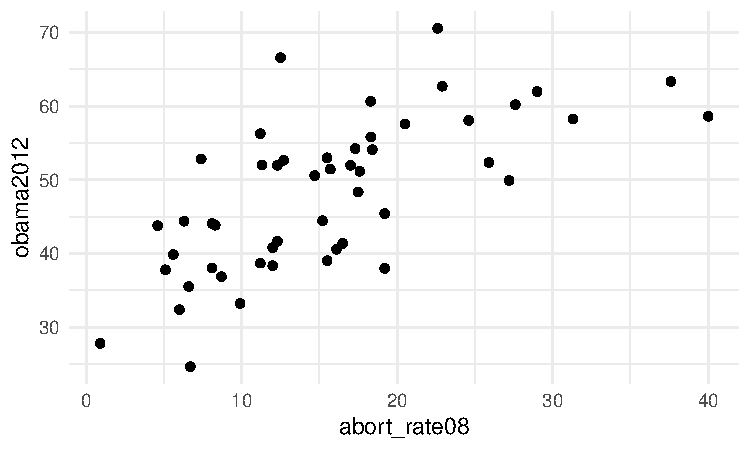
\includegraphics{qpolr_files/figure-latex/unnamed-chunk-199-1.pdf}
  
  \backmatter
  
  \chapter{References}\label{references}
  
  \noindent
  
  \setlength{\parindent}{-0.20in} \setlength{\leftskip}{0.20in}
  \setlength{\parskip}{8pt}
  
  \hypertarget{refs}{}
  \hypertarget{ref-chanetal2016}{}
  Chan, C., Chan, G. C. H., \& Leeper, T. J. (2016). \emph{Rio: A
  swiss-army knife for data file i/o}.
  
  \hypertarget{ref-foxweisberg2011}{}
  Fox, J., \& Weisberg, S. (2011). \emph{An R companion to applied
  regression} (Second). Thousand Oaks CA: Sage. Retrieved from
  \url{http://socserv.socsci.mcmaster.ca/jfox/Books/Companion}
  
  \hypertarget{ref-healymoody2014}{}
  Healy, K., \& Moody, J. (2014). Data visualization in sociology.
  \emph{Annual Review of Sociology}, \emph{40}, 105--128.
  
  \hypertarget{ref-rtweet-package}{}
  Kearney, M. W. (2018). \emph{Rtweet: Collecting twitter data}. Retrieved
  from \url{https://cran.r-project.org/package=rtweet}
  
  \hypertarget{ref-larsen2018}{}
  Larsen, E. G. (2018). Welfare retrenchments and government support:
  Evidence from a natural experiment. \emph{European Sociological Review},
  \emph{34}(1), 40--51.
  
  \hypertarget{ref-rcoreteam2015foreign}{}
  R Core Team. (2015). \emph{Foreign: Read data stored by minitab, s, sas,
  spss, stata, systat, weka, dBase, ...} Retrieved from
  \url{http://CRAN.R-project.org/package=foreign}
  
  \hypertarget{ref-Robinson2018}{}
  Robinson, D. (2018). \emph{Broom: Convert statistical analysis objects
  into tidy data frames}. Retrieved from
  \url{https://CRAN.R-project.org/package=broom}
  
  \hypertarget{ref-tidytext2016}{}
  Silge, J., \& Robinson, D. (2016). Tidytext: Text mining and analysis
  using tidy data principles in r. \emph{JOSS}, \emph{1}(3).
  \url{http://doi.org/10.21105/joss.00037}
  
  \hypertarget{ref-tufte1983}{}
  Tufte, E. R. (1983). \emph{The visual display of quantitative
  information}. Graphics Press.
  
  \hypertarget{ref-wickham2009}{}
  Wickham, H. (2009). \emph{Ggplot2: Elegant graphics for data analysis}.
  Springer-Verlag New York. Retrieved from \url{http://ggplot2.org}
  
  \hypertarget{ref-wickham2017}{}
  Wickham, H. (2017). \emph{Tidyverse: Easily install and load the
  'tidyverse'}. Retrieved from
  \url{https://CRAN.R-project.org/package=tidyverse}
  
  \hypertarget{ref-wickhamfrancois2015}{}
  Wickham, H., \& Francois, R. (2015). \emph{Readr: Read tabular data}.
  Retrieved from \url{http://CRAN.R-project.org/package=readr}
  
  \hypertarget{ref-wickhamfrancois2016}{}
  Wickham, H., \& Francois, R. (2016). \emph{Dplyr: A grammar of data
  manipulation}. Retrieved from
  \url{http://CRAN.R-project.org/package=dplyr}


  % Index?

\end{document}
